\subsection{Информатика}
	
	\subsubsection{Аннотация}

        Курс <<Информатика>> получил в основном положительные отзывы.

        На лекции Дивари И.Н. было получено много развернутых отзывов. Совет студентов и аспирантов ФРКТ считает полезным донесение их до лектора.

        Семинаристы Дединский И.Р., Винокуров Н.А. получили крайне положительные оценки от респондентов. Совет студентов и аспирантов ФРКТ предлагает поощрить перечисленных преподавателей.

        Семинарист Кулиев Р.С. получил негативные отзывы. Респонденты отметили, что преподаватель постоянно пропускает семинары. Совет студентов и аспирантов ФРКТ рекомендует заменить этого семинариста.
        
        Кроме того, респонденты отметили, что контрольная работа была плохо организована.

	\subsubsection{Общий отзыв студентов о курсе}

		\begin{figure}[H]
			\centering
			\begin{subfigure}[b]{0.45\textwidth}
				\centering
				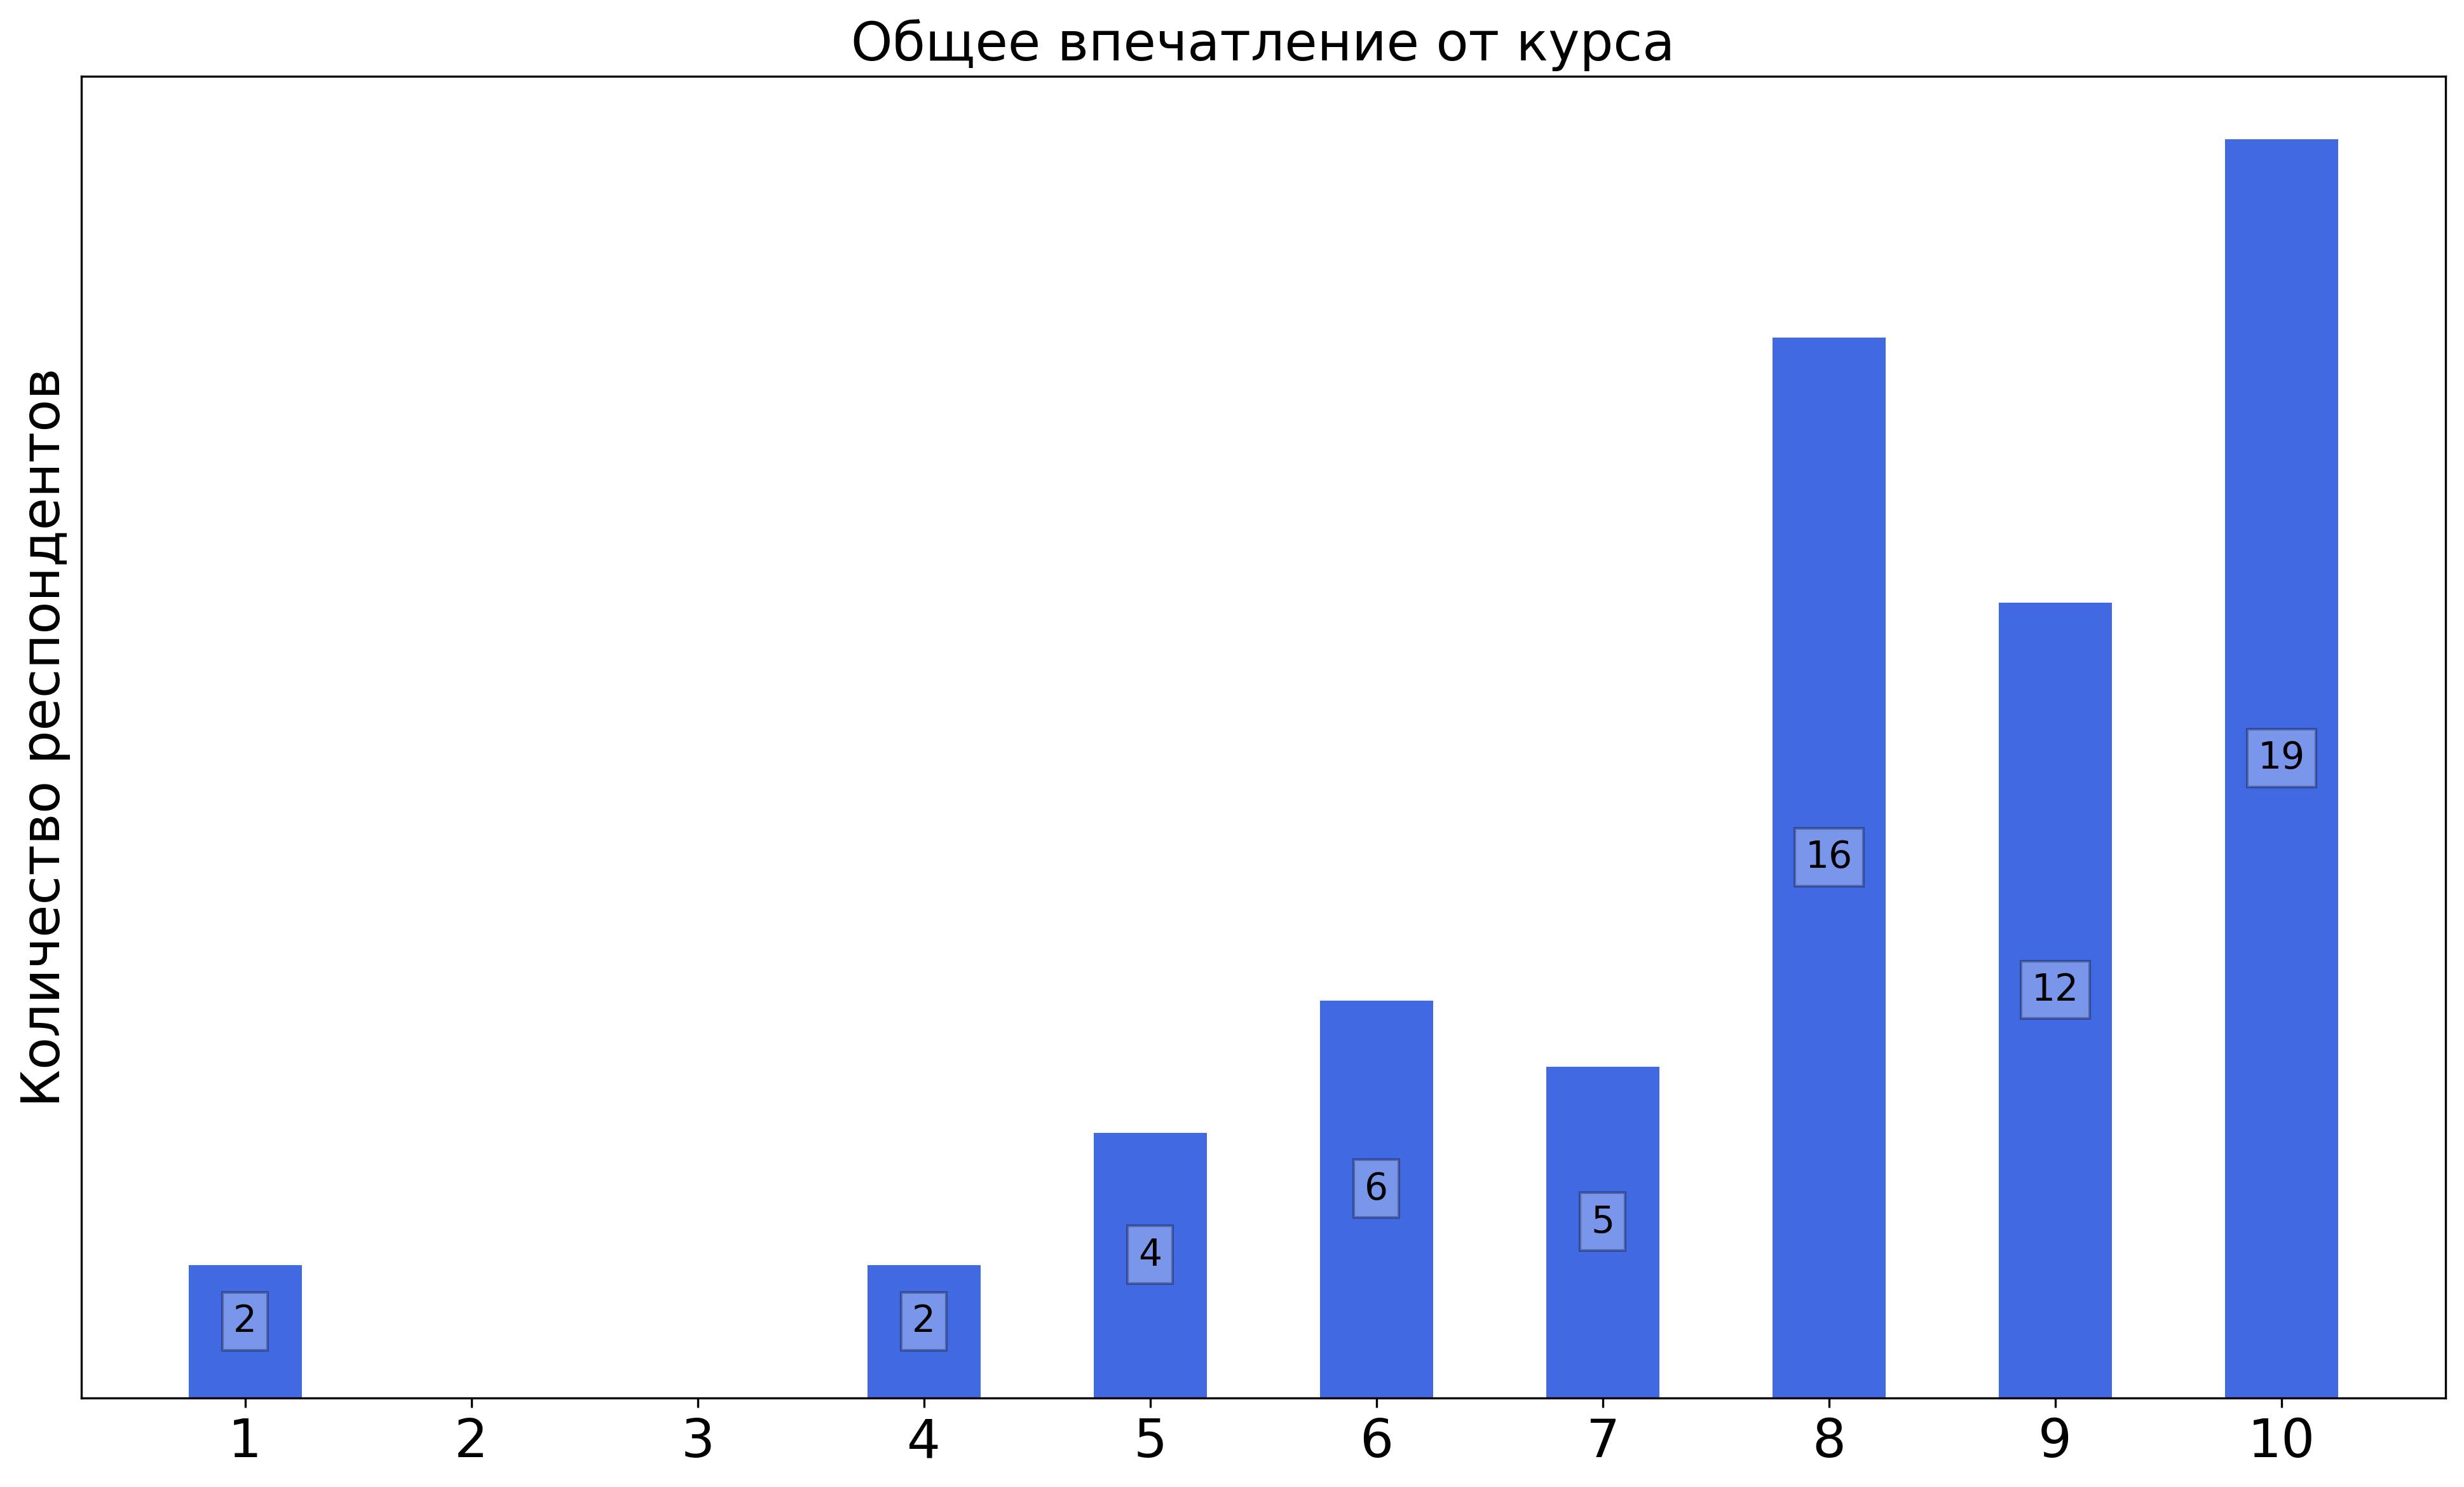
\includegraphics[width=\textwidth]{images/1 course/Информатика/general-0.png}
			\end{subfigure}
		\end{figure}

	\subsubsection{Материалы, использумые респондентами при изучении курса}

		\begin{figure}[H]
			\centering
			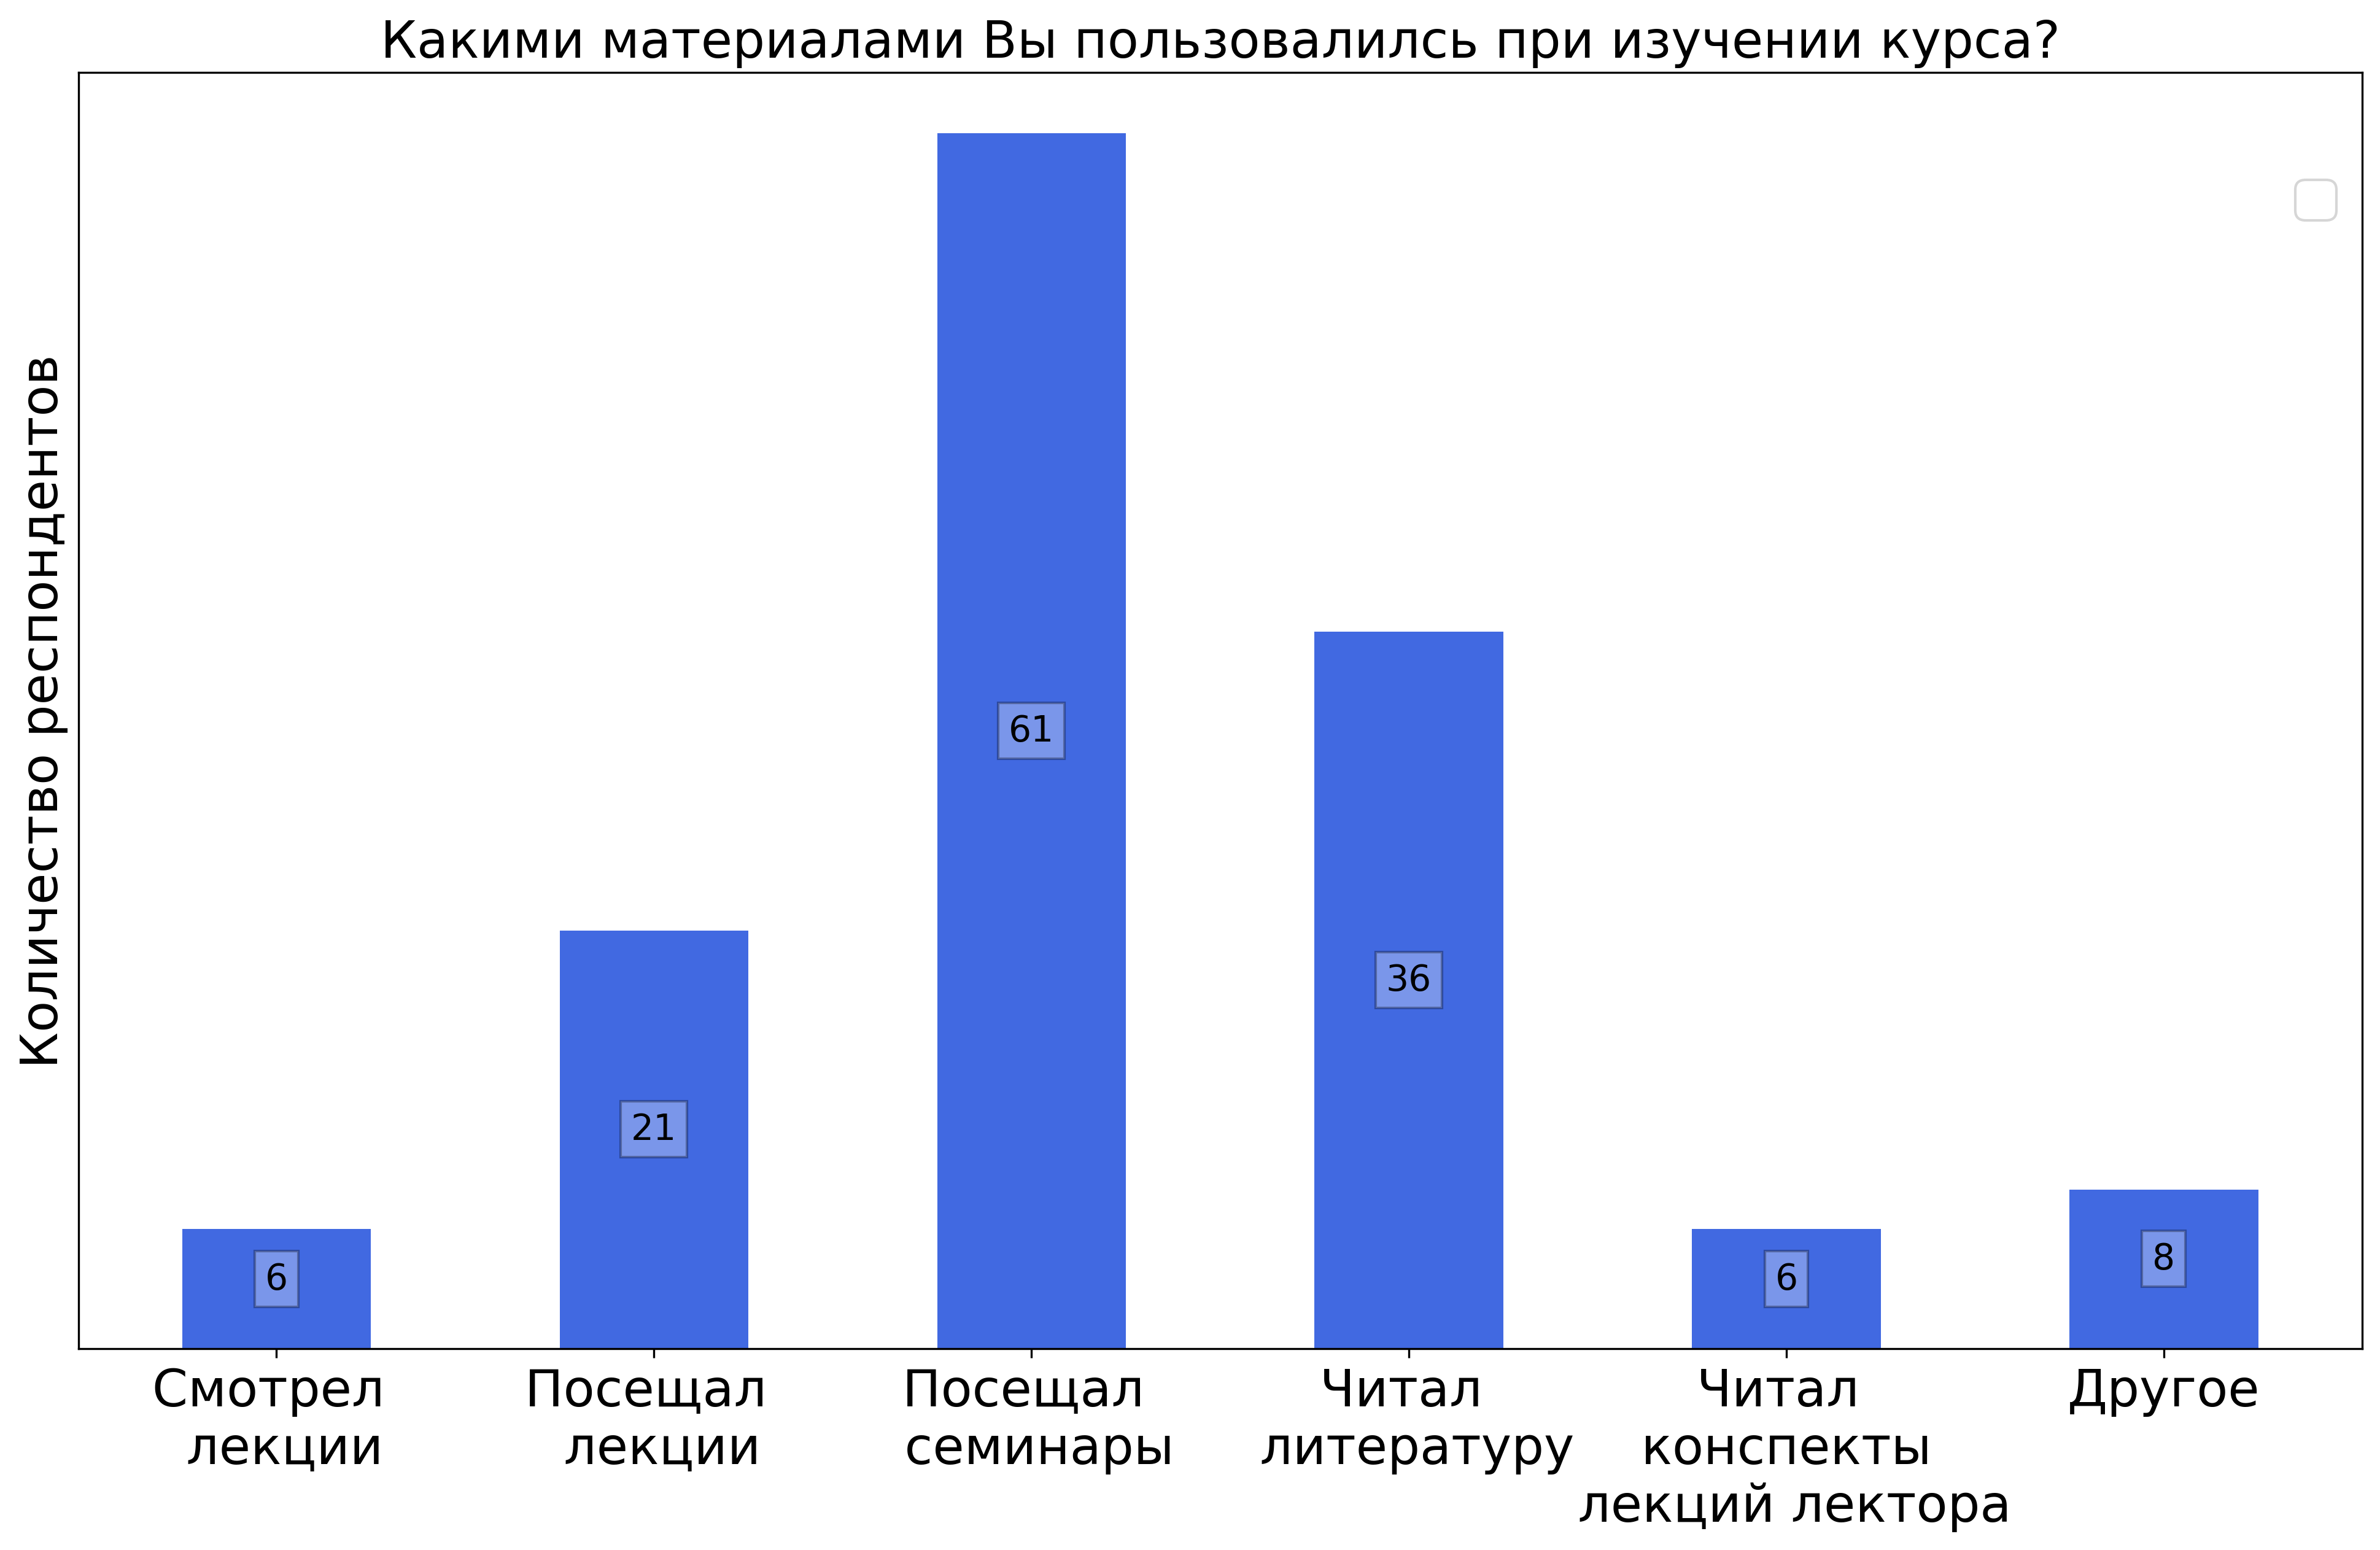
\includegraphics[width = 0.45\textwidth]{images/1 course/Информатика/materials.png}
		\end{figure}

		\textit{В качестве других источников информации студенты указали:} 
		\begin{itemize}
			\item доп. курс Дединского И.Р.;
			\item материалы из интернета.
		\end{itemize}

	\subsubsection{Отзыв студентов о лекциях. Лектор: Дивари И.Н.}

		\begin{figure}[H]
			\centering
            \begin{subfigure}[b]{0.45\textwidth}
				\centering
				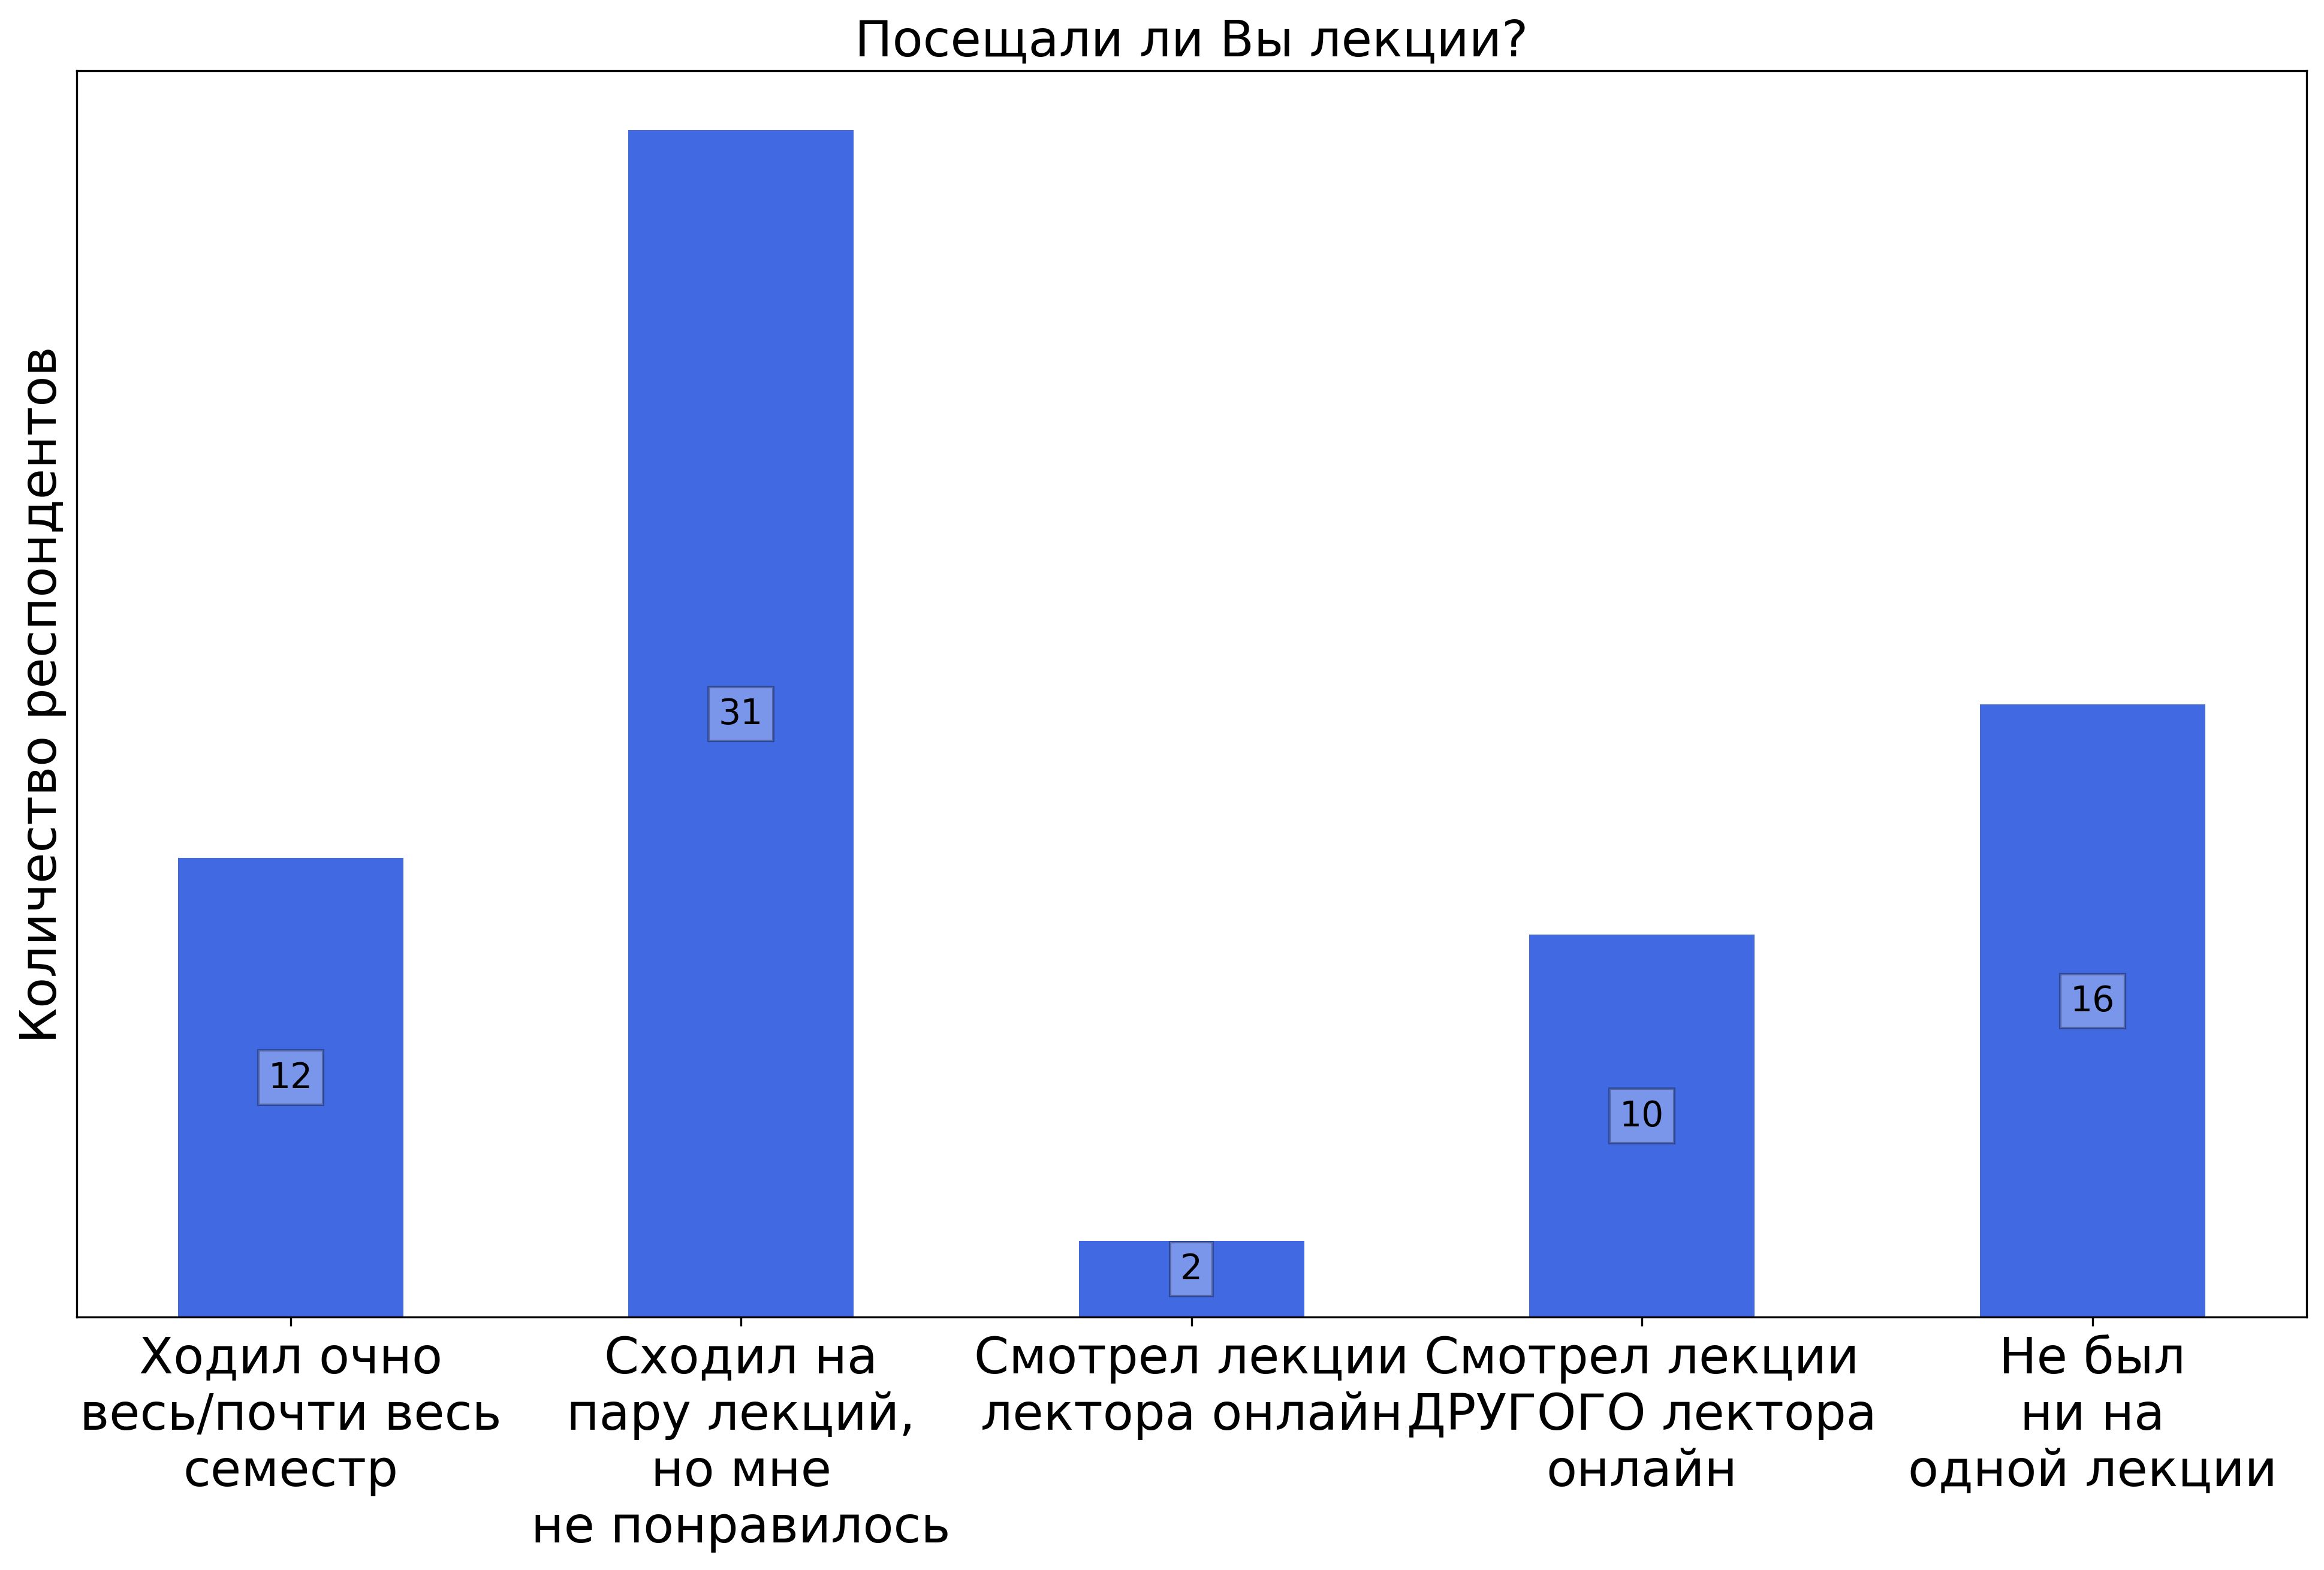
\includegraphics[width=\textwidth]{images/1 course/Информатика/lecturer-questions-Дивари И.Н.-0.png}
			\end{subfigure}
			\begin{subfigure}[b]{0.45\textwidth}
				\centering
				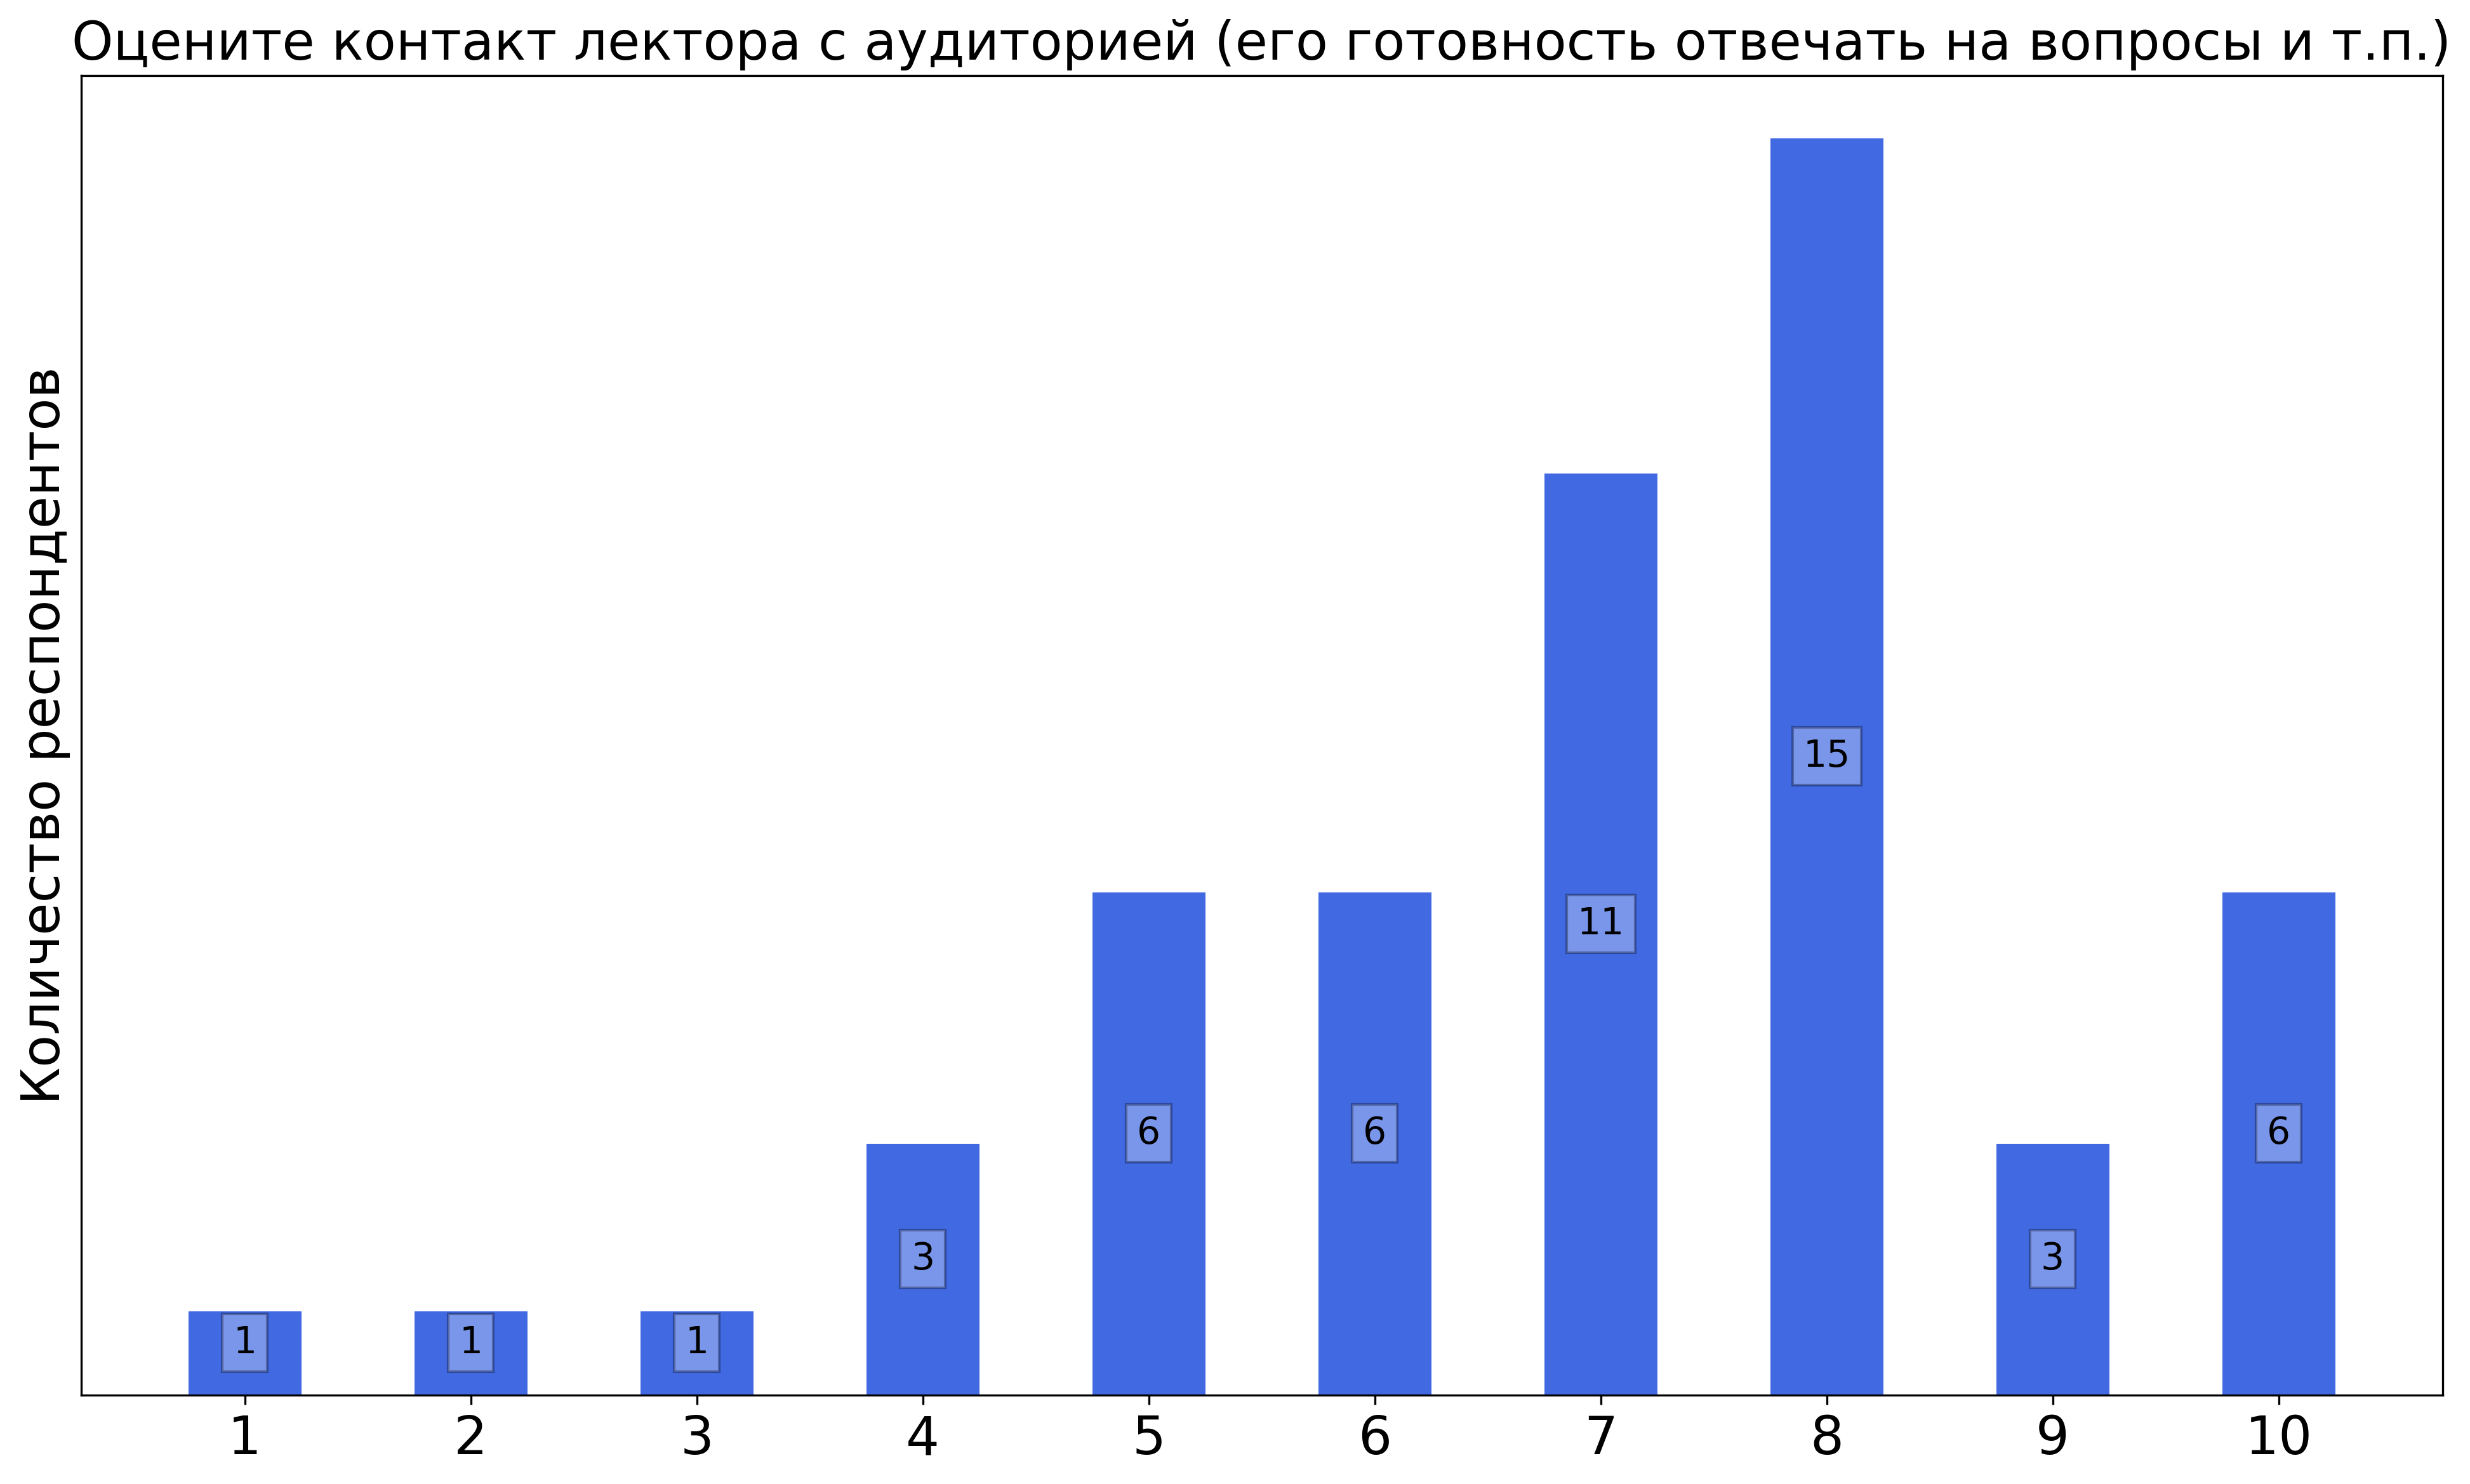
\includegraphics[width=\textwidth]{images/1 course/Информатика/lecturer-marks-Дивари И.Н.-0.png}
			\end{subfigure}
			\begin{subfigure}[b]{0.45\textwidth}
				\centering
				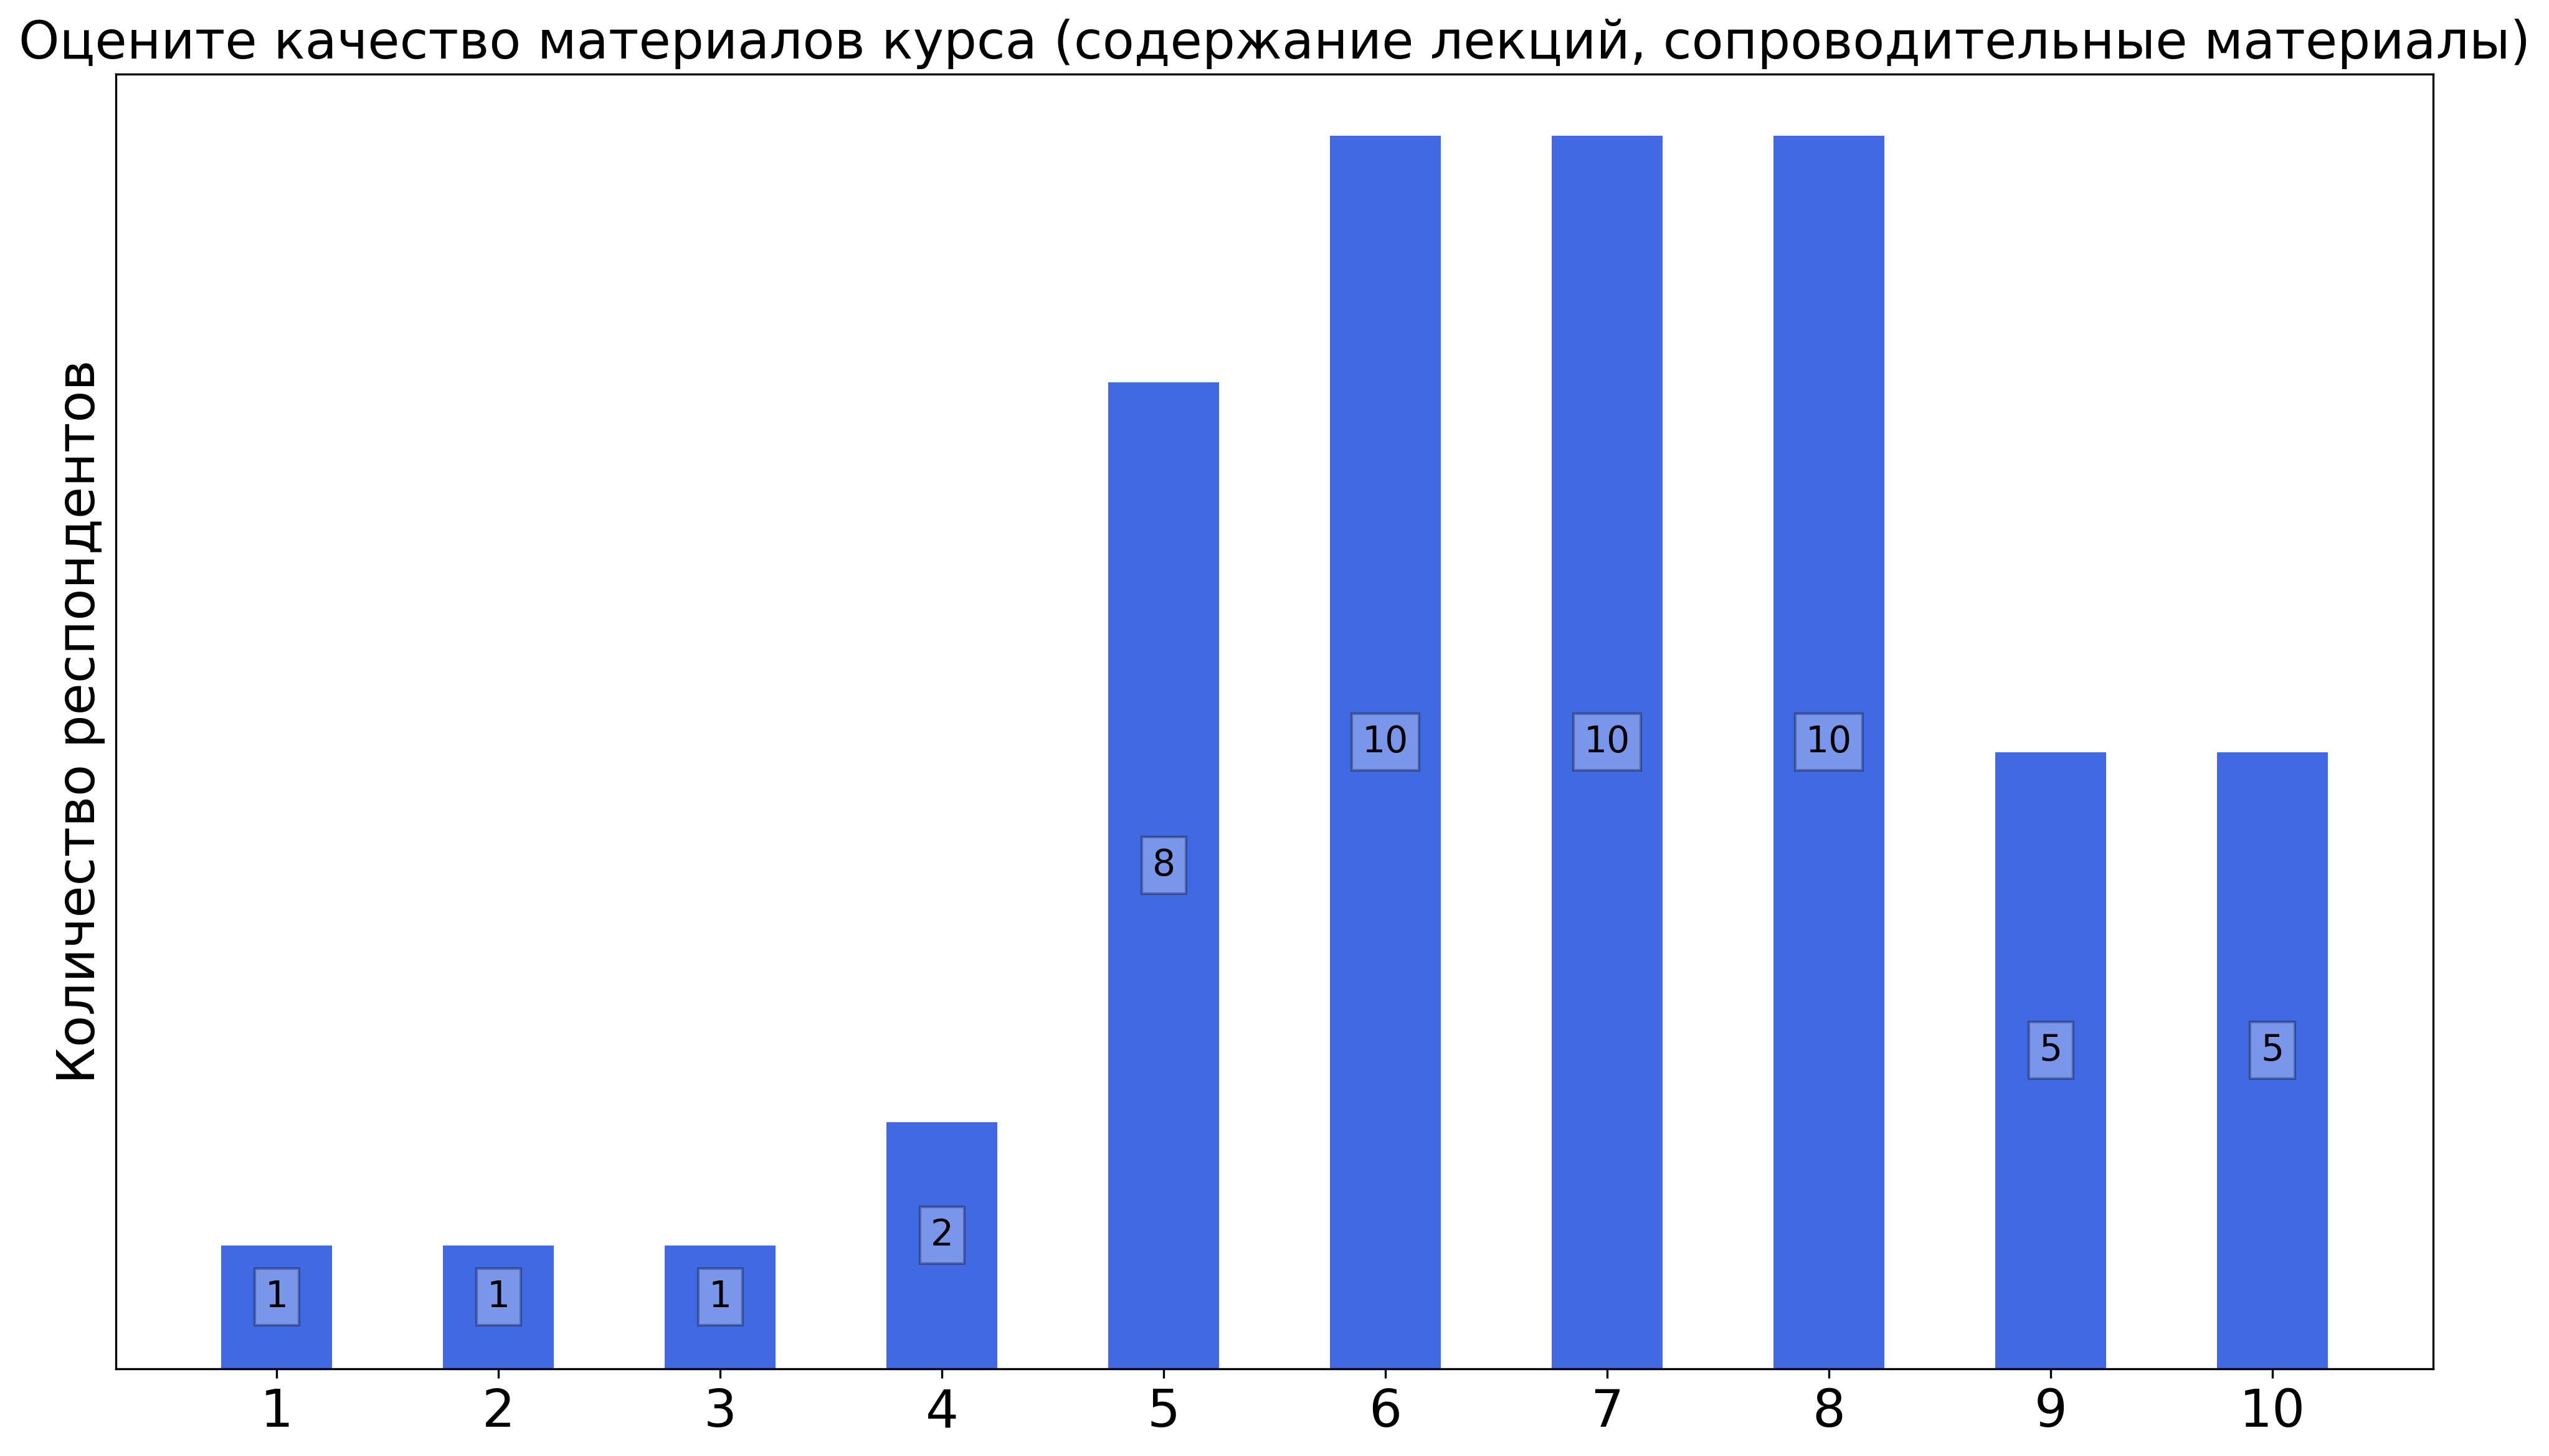
\includegraphics[width=\textwidth]{images/1 course/Информатика/lecturer-marks-Дивари И.Н.-1.png}
			\end{subfigure}
			\begin{subfigure}[b]{0.45\textwidth}
				\centering
				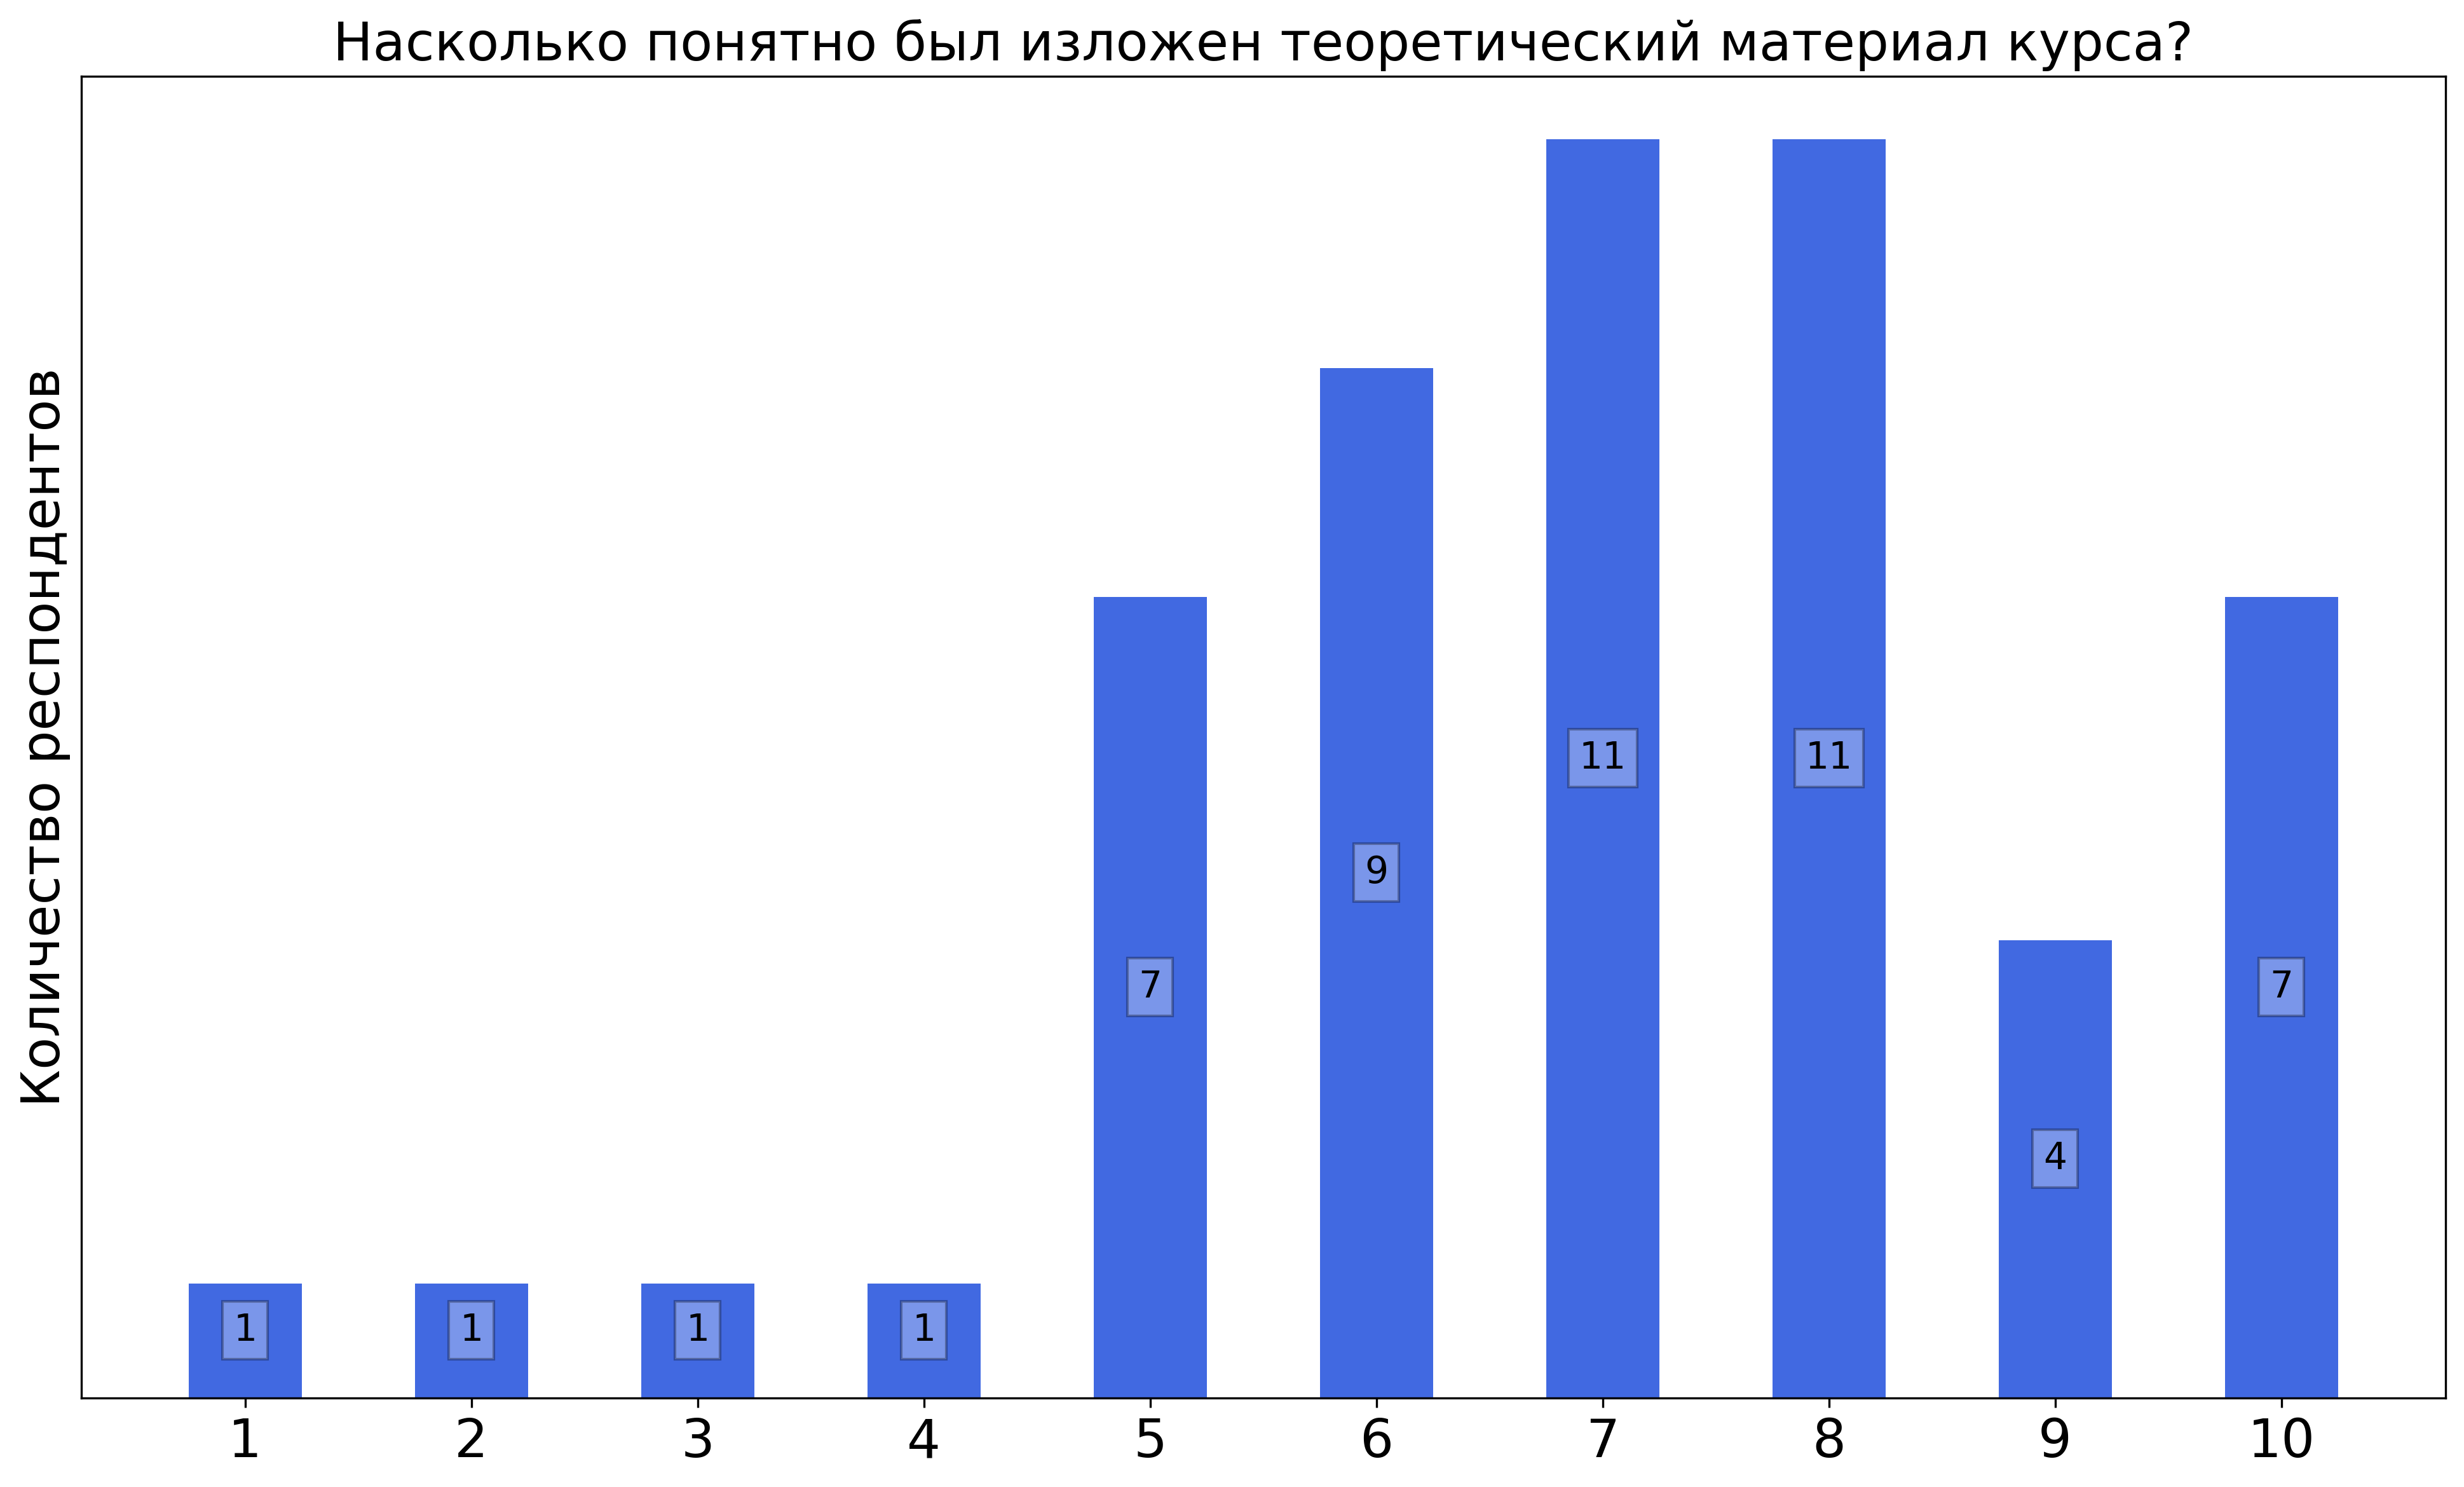
\includegraphics[width=\textwidth]{images/1 course/Информатика/lecturer-marks-Дивари И.Н.-2.png}
			\end{subfigure}
			\begin{subfigure}[b]{0.45\textwidth}
				\centering
				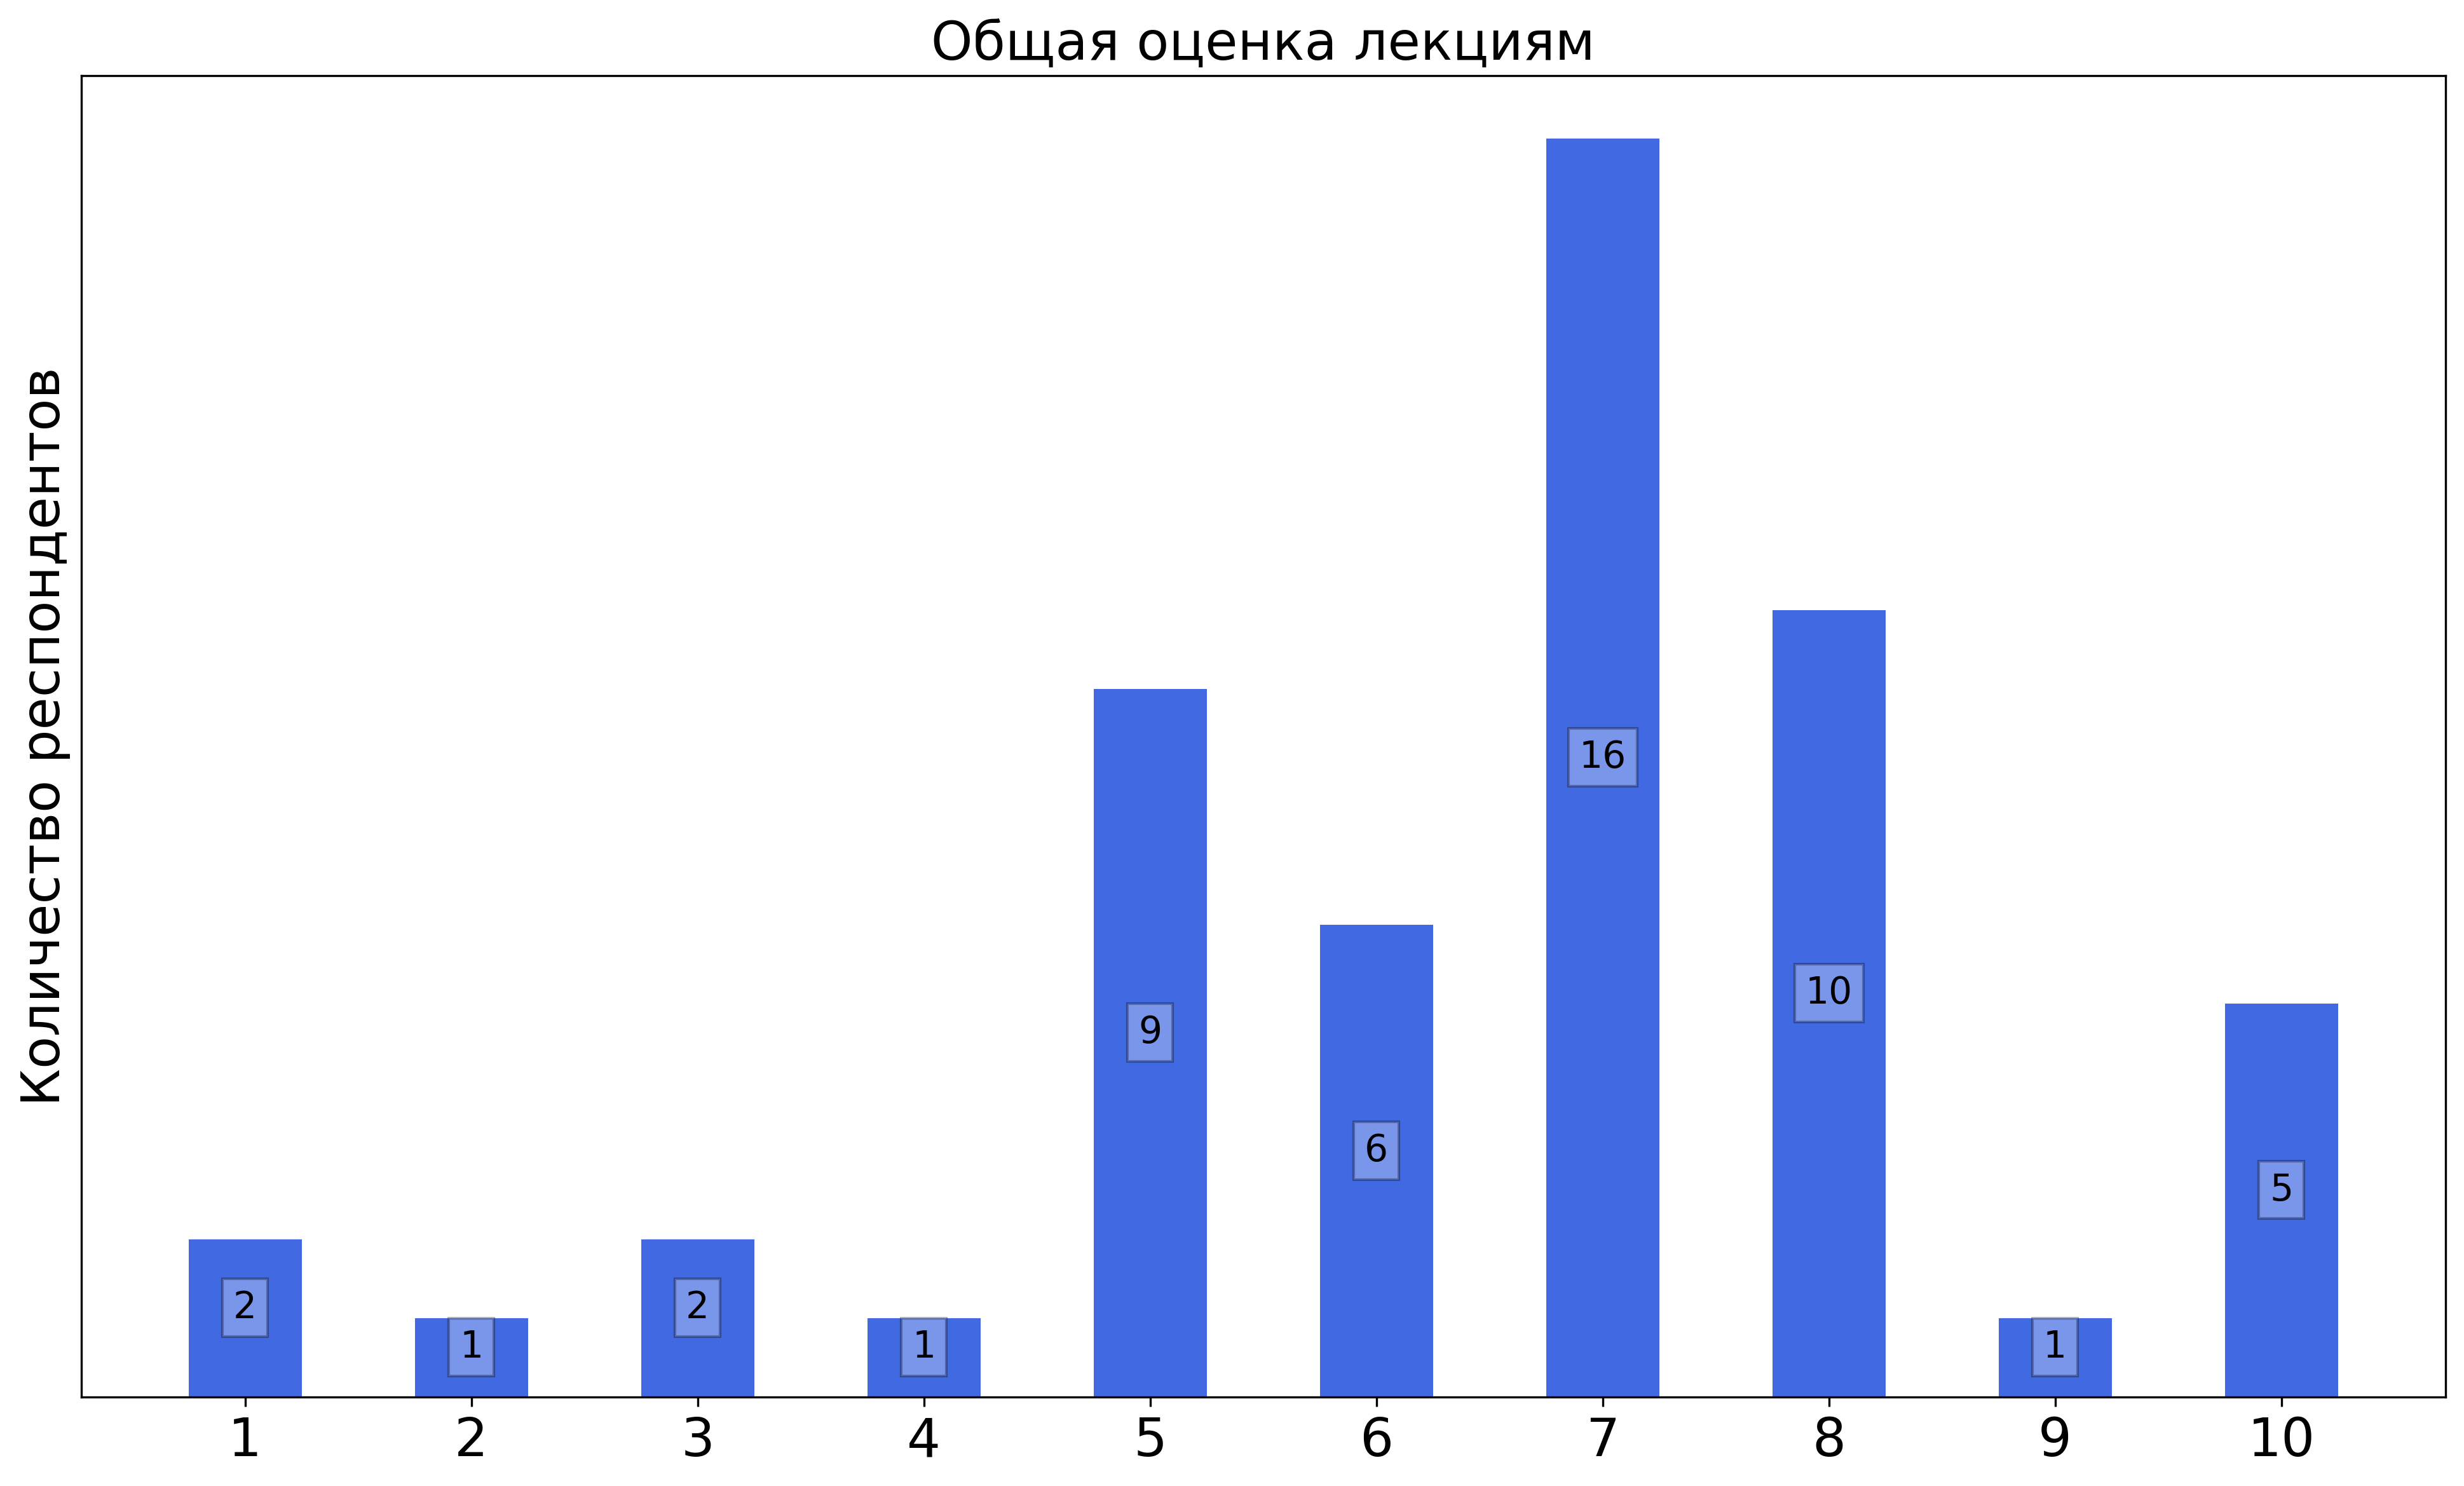
\includegraphics[width=\textwidth]{images/1 course/Информатика/lecturer-marks-Дивари И.Н.-3.png}
			\end{subfigure}
			\caption{Оценки респондентов о качестве преподавания лекций по курсу <<Информатика>>}
		\end{figure}

		\textbf{Комментарии студентов о лекциях\protect\footnote{сохранены оригинальные орфография и пунктуация}}    
            \begin{commentbox} 
                Хуавей заменил мне Дивари 
            \end{commentbox} 
        
            \begin{commentbox} 
                просто читает слайды с презентации 
            \end{commentbox} 
        
            \begin{commentbox} 
                Самые бесполезные лекции. На них мало кто ходил, потому что всю инфу по сути знали. Слышал, что были какие-то даже алгоритмы, но никто не знал, что они будут. Лучше б сделали курс по алгосам. Понятно, что предназначено для тех, кто не ходил к деду, но тогда зачем было вообще поступать?  
            \end{commentbox} 
        
            \begin{commentbox} 
                На первой же лекции мы были без перерыва (с согласия аудитории), однако и этого времени ей не хватило чтобы закончить вовремя, и ещё 5 минут перемены пришлось потратить. Не совсем понятна цель такого - ей оставалось рассказать про машину Тьюринга и полностью про машину Поста, к чему спешка за 5 минут все рассказать не очевидно
            \end{commentbox} 
        
            \begin{commentbox} 
                Хорошо ведёт лекции 
            \end{commentbox} 
        
            \begin{commentbox} 
                К лектору вопросов нет. Почти не ходил на лекции, потому что потребность в сне была больше, чем потребность в лекциях. 
            \end{commentbox} 
        
            \begin{commentbox} 
                В целом есть доля полезного, но много лишнего 
            \end{commentbox} 
        
            \begin{commentbox} 
                На её лекциях хочется спать, но рассказывает много нужной информации, но очень нудно 
            \end{commentbox} 
        
            \begin{commentbox} 
                Был на нескольких лекциях, но в группе Деда особого смысла ходить на них не видел. 
            \end{commentbox} 
    
    
    \subsubsection{Отзыв студентов о семинарах. Семинарист: Дединский И.Р.}
		\begin{figure}[H]
			\centering
			\begin{subfigure}[b]{0.45\textwidth}
				\centering
				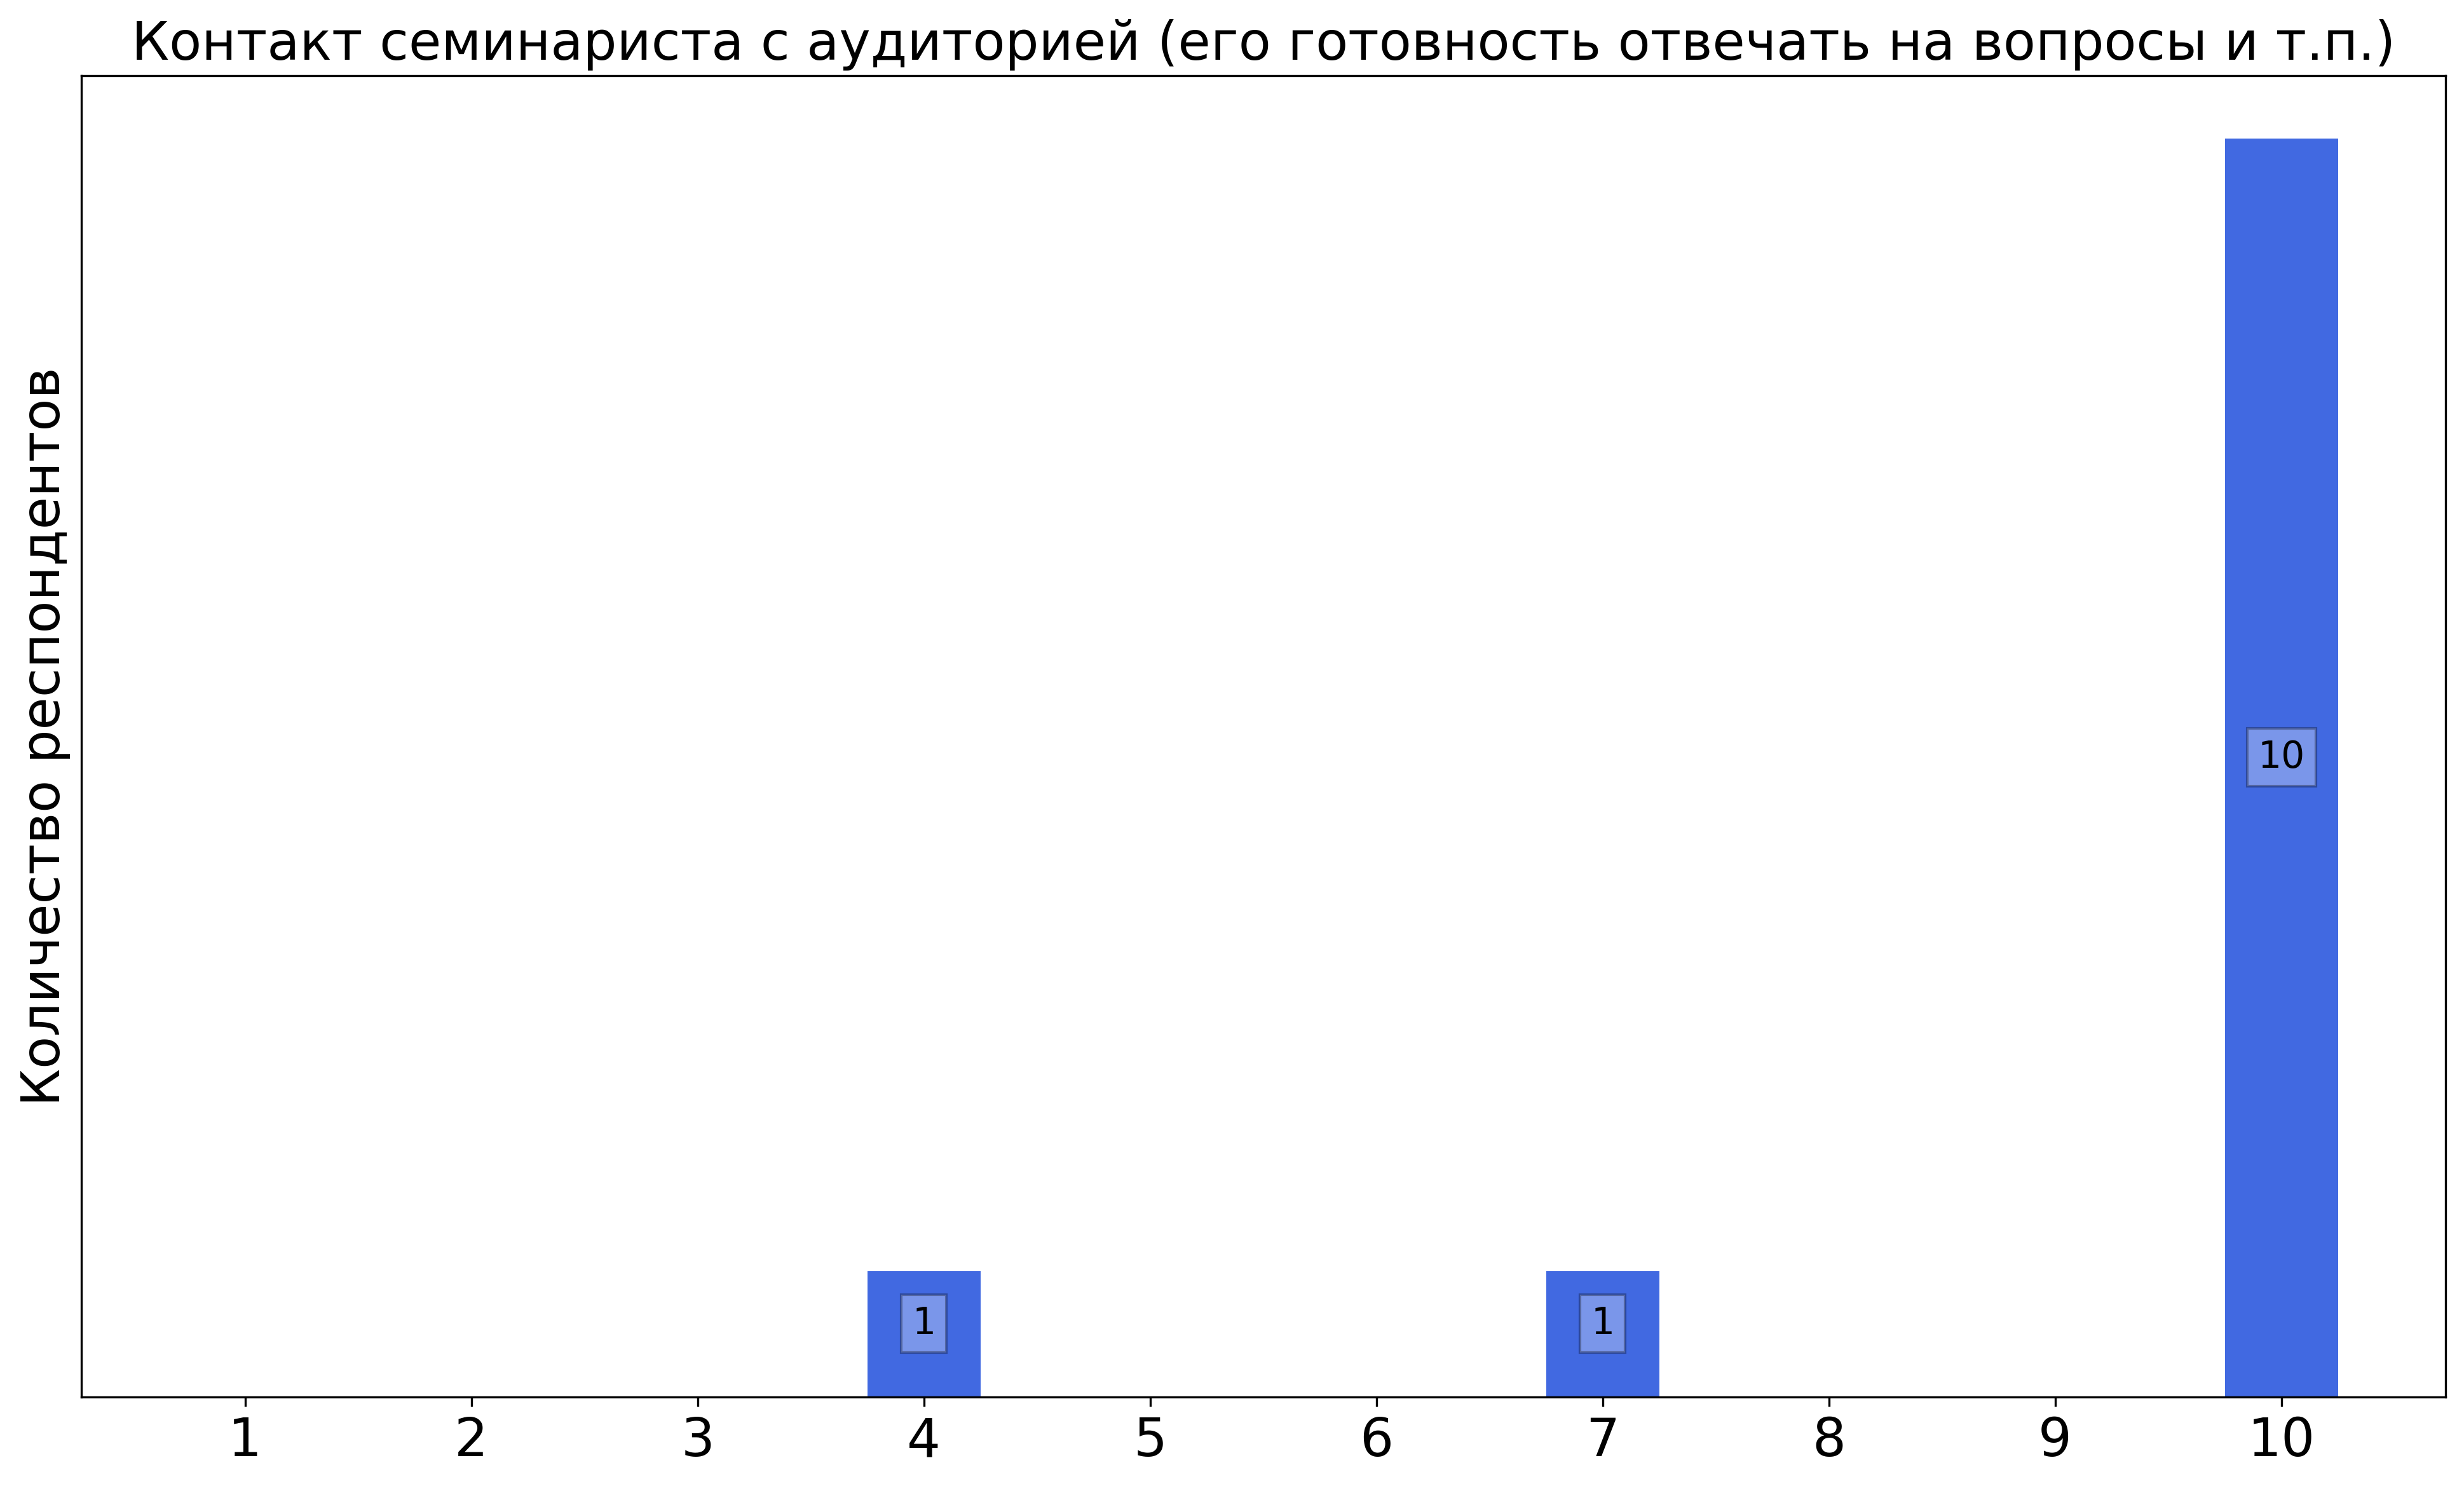
\includegraphics[width=\textwidth]{images/1 course/Информатика/seminarists-marks-Дединский И.Р.-0.png}
			\end{subfigure}
			\begin{subfigure}[b]{0.45\textwidth}
				\centering
				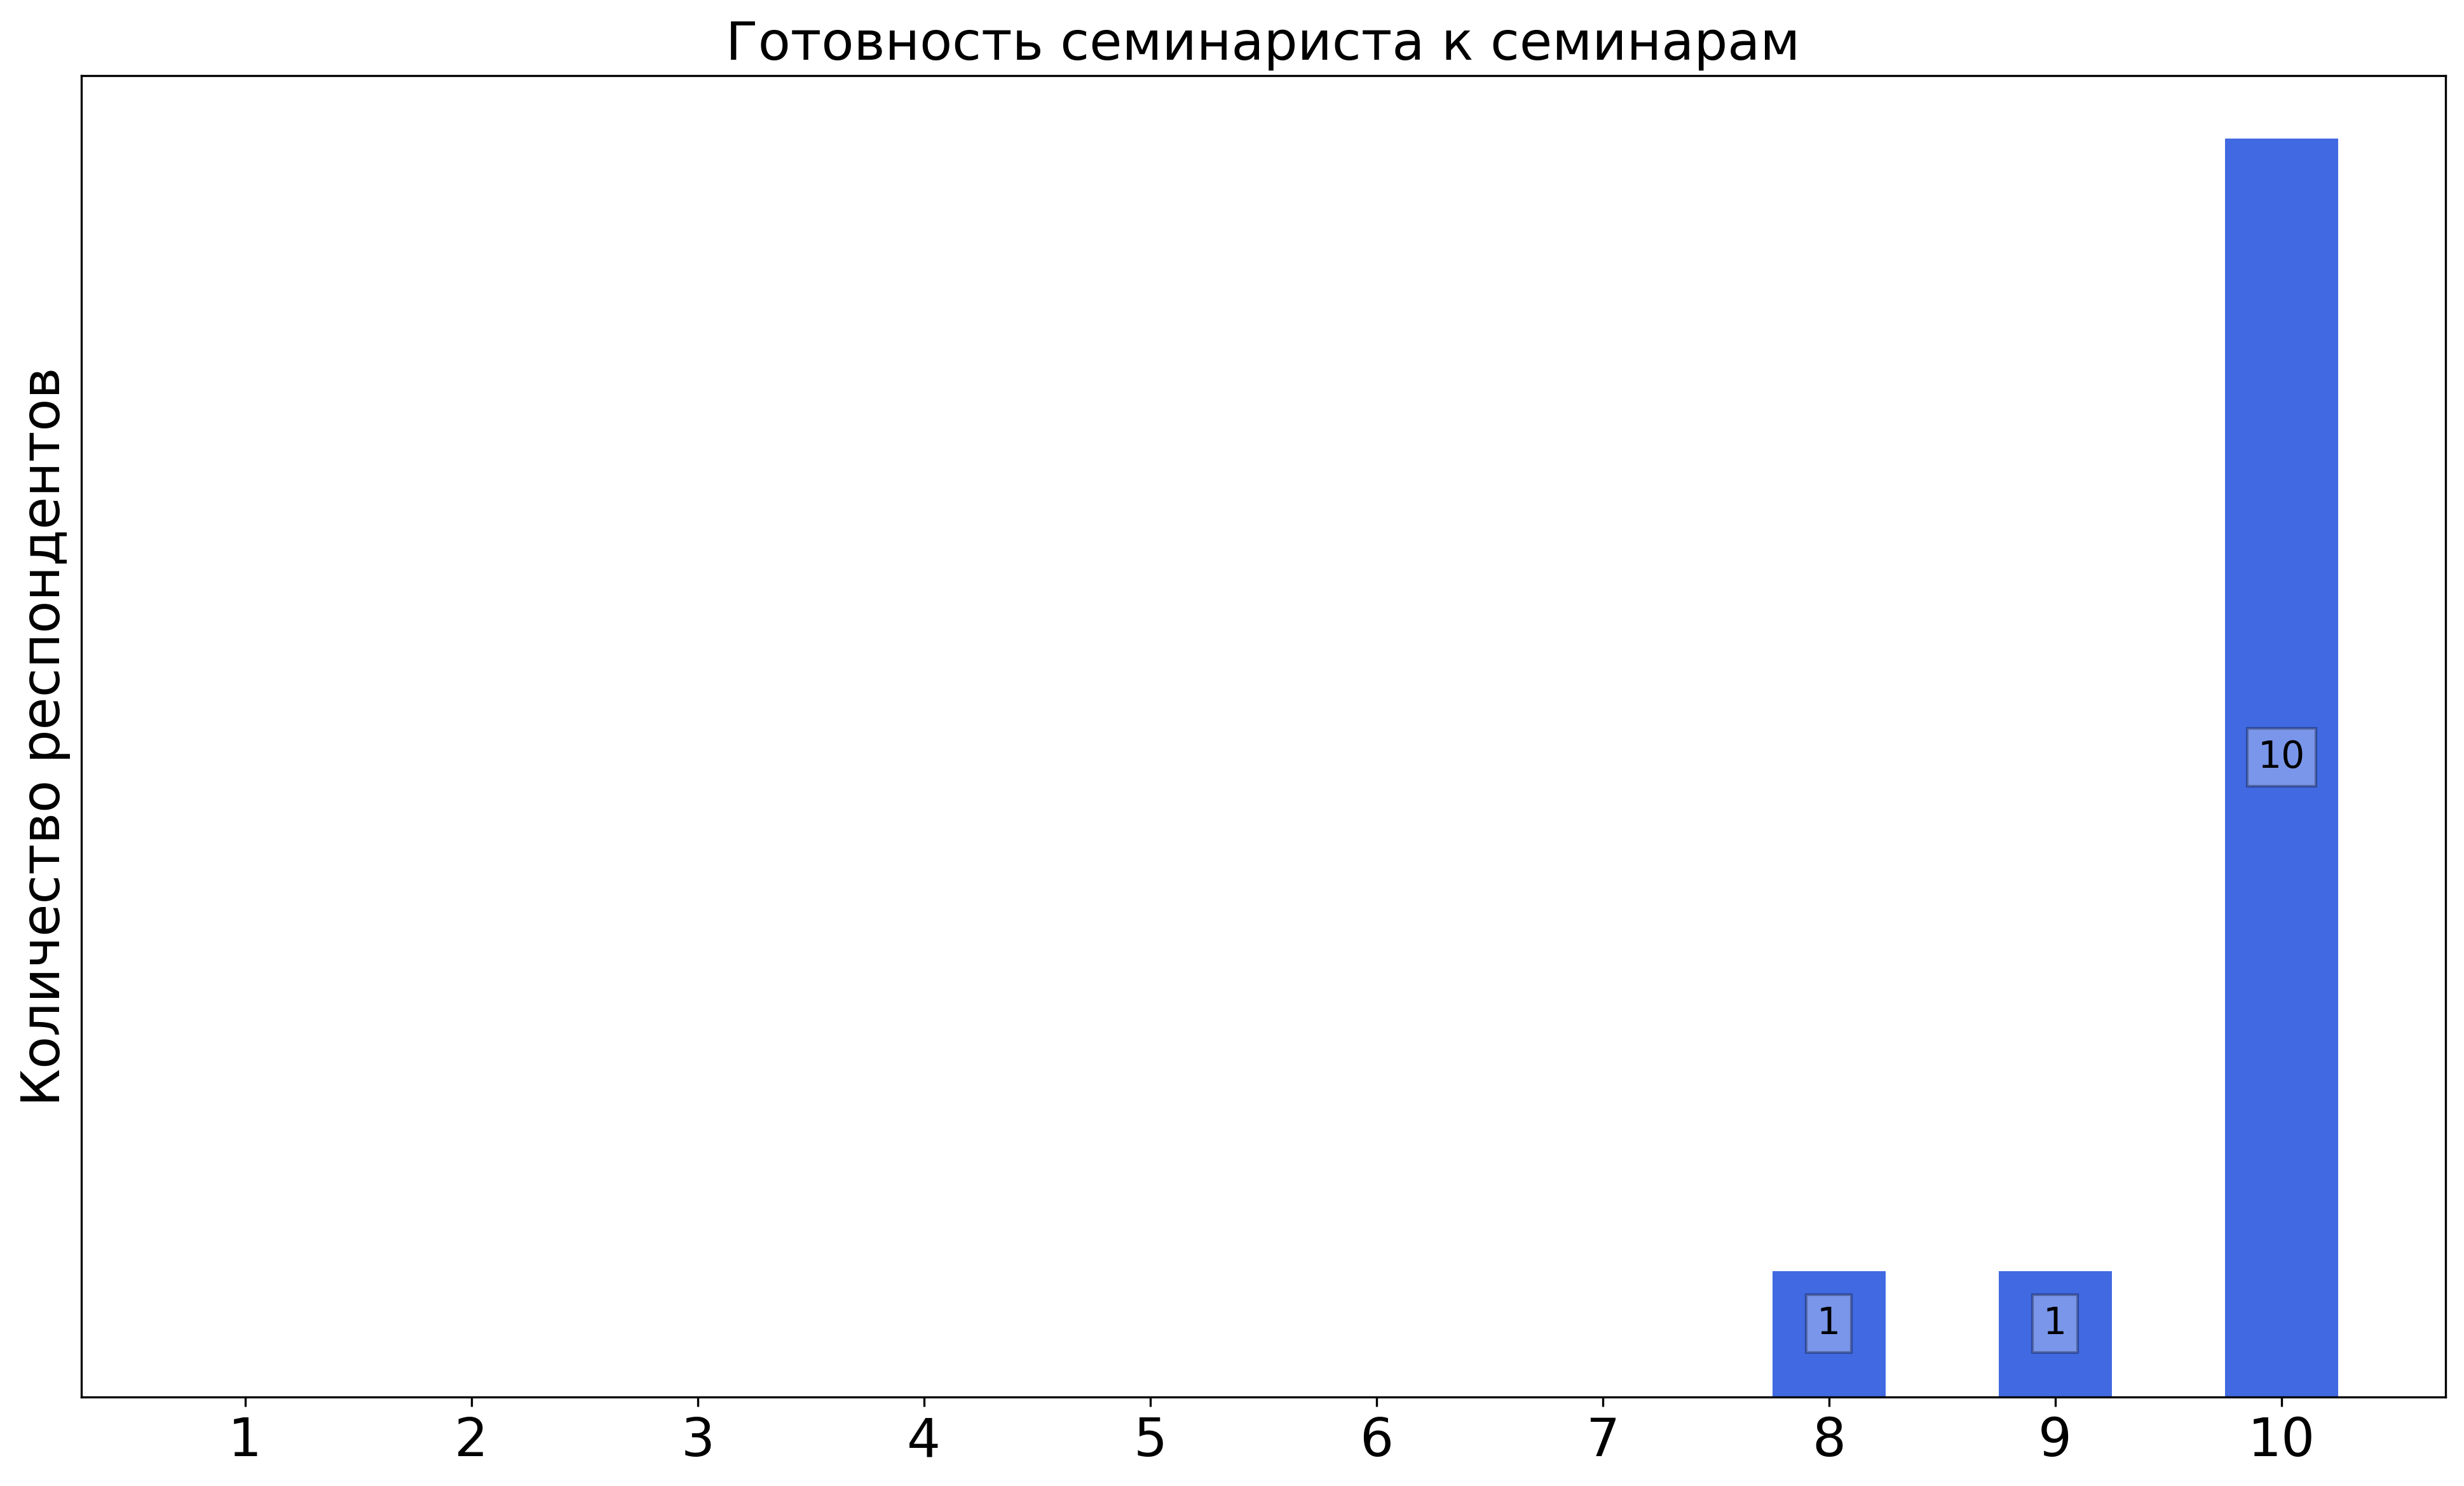
\includegraphics[width=\textwidth]{images/1 course/Информатика/seminarists-marks-Дединский И.Р.-1.png}
			\end{subfigure}
			\begin{subfigure}[b]{0.45\textwidth}
				\centering
				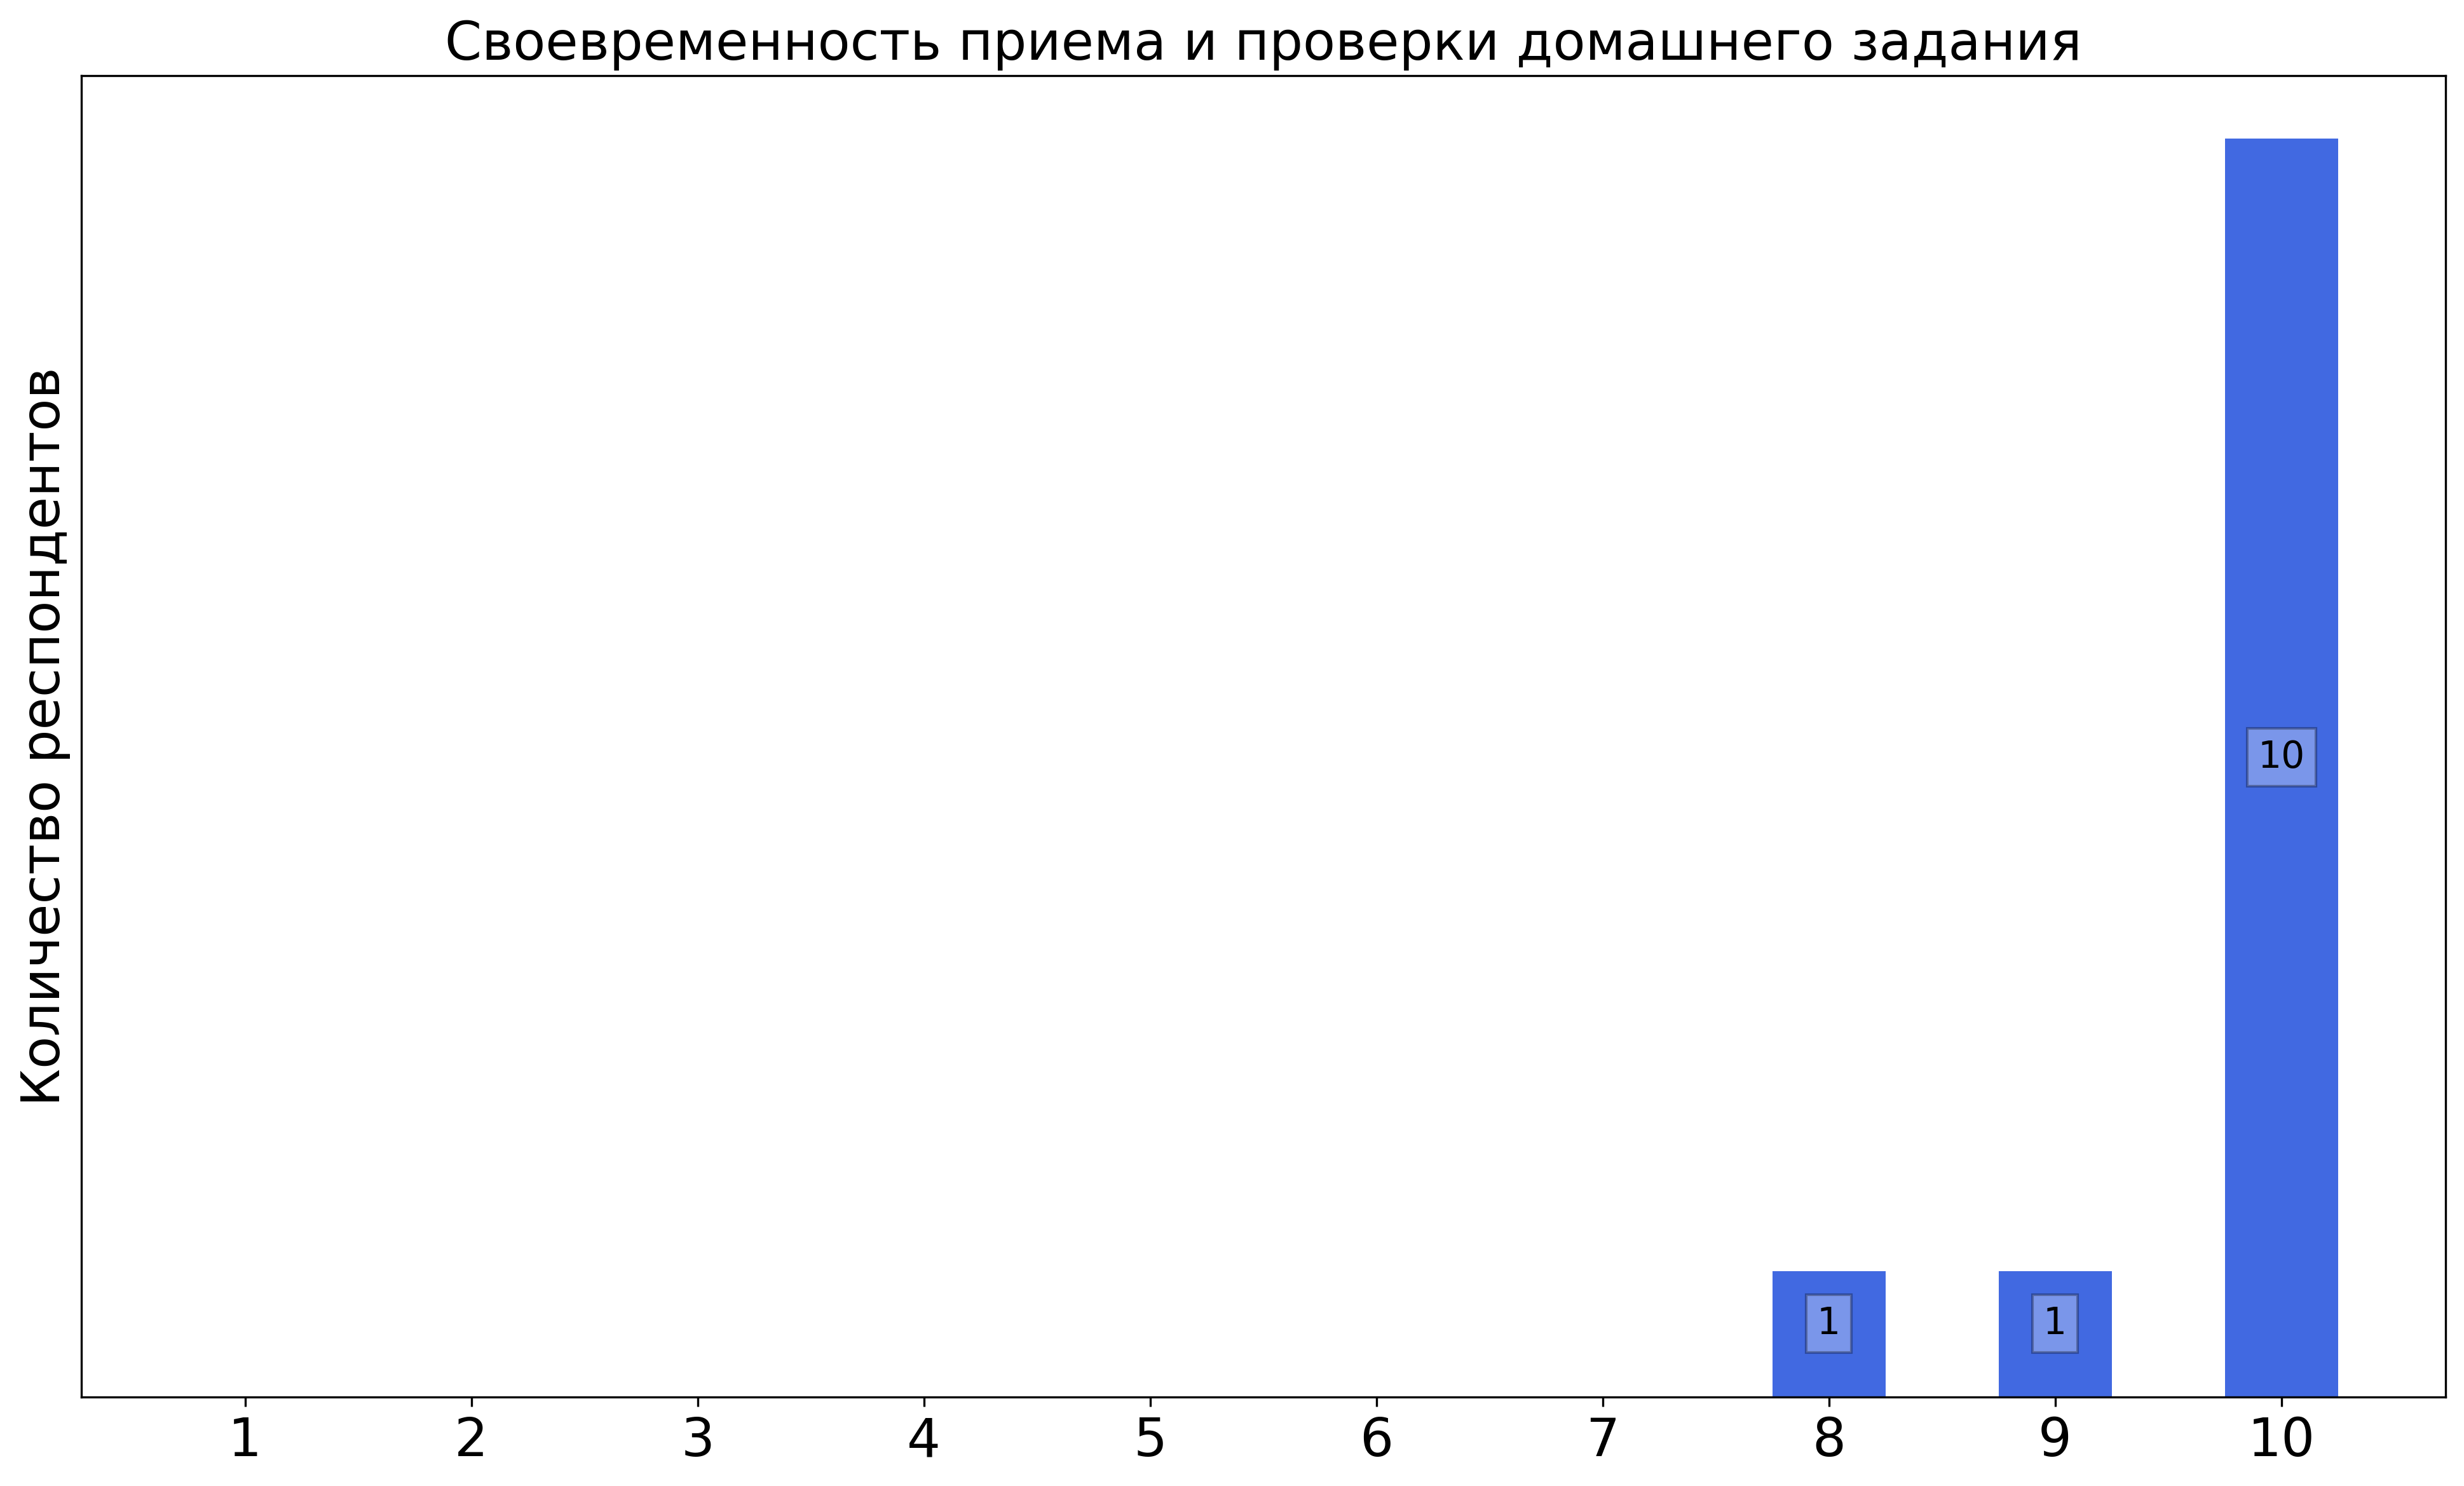
\includegraphics[width=\textwidth]{images/1 course/Информатика/seminarists-marks-Дединский И.Р.-2.png}
			\end{subfigure}
			\begin{subfigure}[b]{0.45\textwidth}а
				\centering
				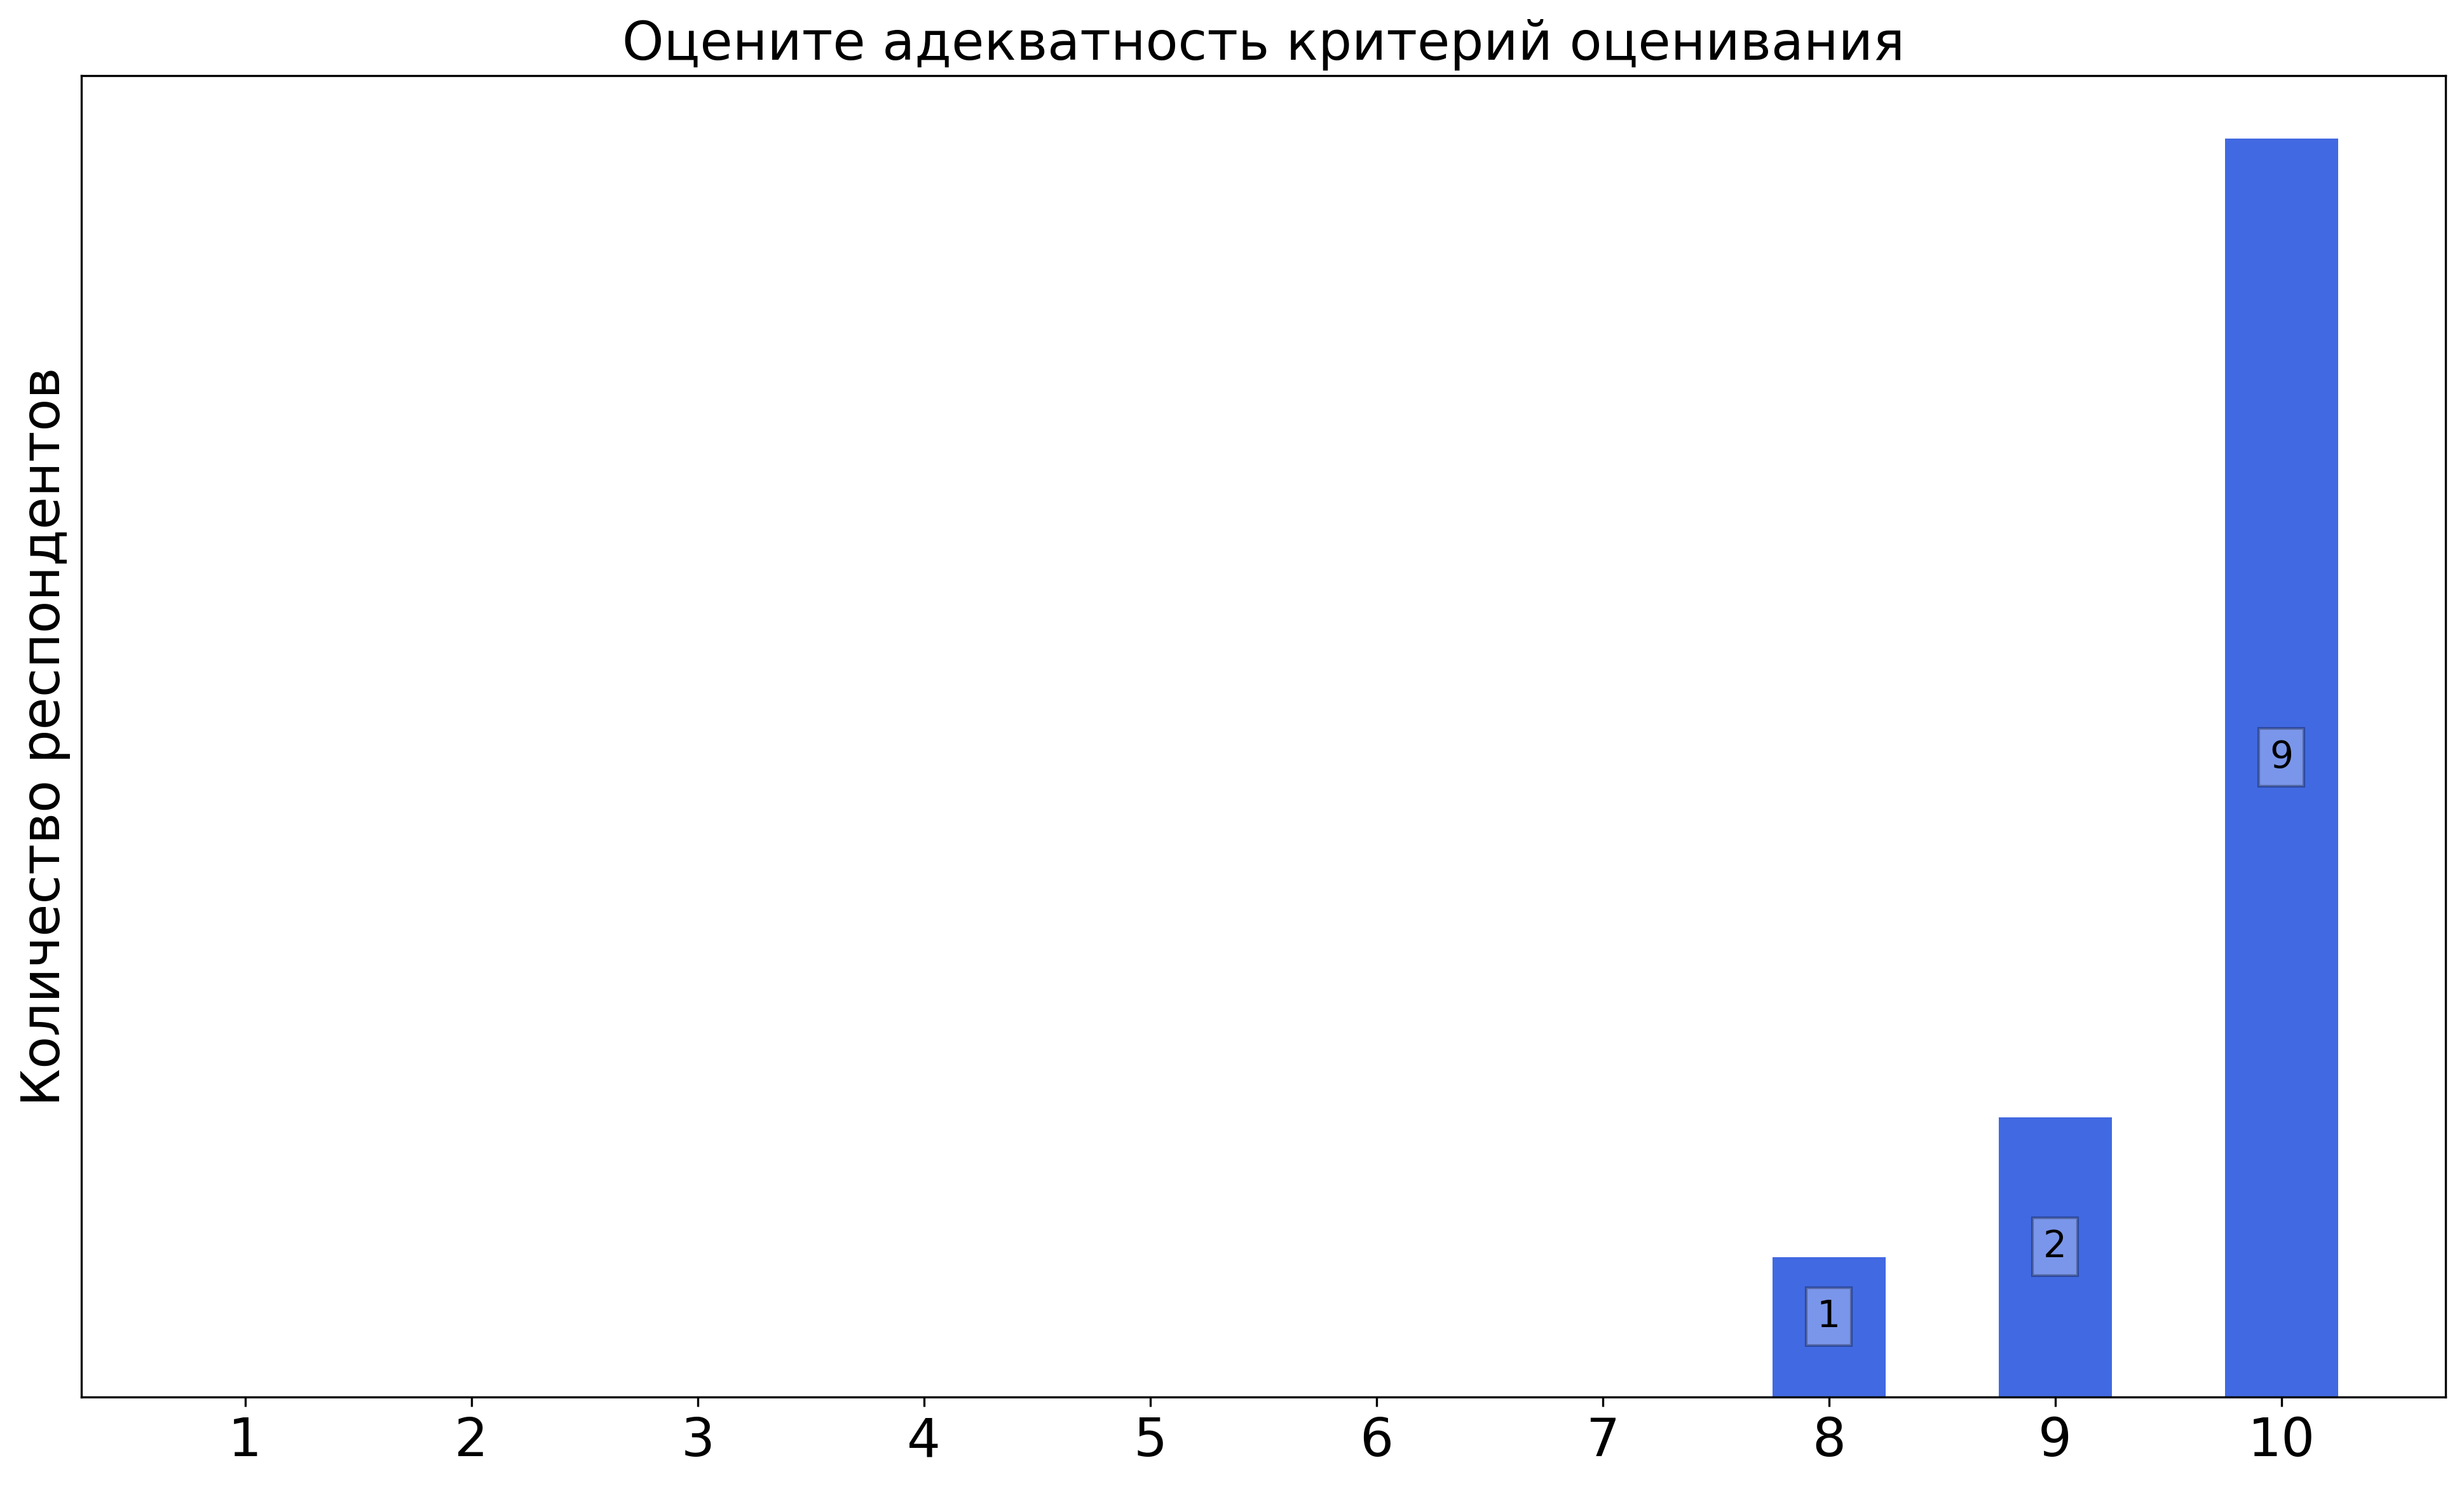
\includegraphics[width=\textwidth]{images/1 course/Информатика/seminarists-marks-Дединский И.Р.-3.png}
			\end{subfigure}	
			\caption{Оценки респондентов о качестве преподавания семинаров}
		\end{figure}

		\textbf{Комментарии студентов о семинаристе\protect\footnote{сохранены оригинальные орфография и пунктуация}}
            \begin{commentbox} 
                Самые крутые семинары на физтехе. Очень много интересной инфы. Расшаривает, если правильно спросить. Заставляет действительно думать, а не просто сидеть и молчать. Требовательно, зато действительно учишься разбираться в вопросе и заниматься делом. 
            \end{commentbox} 
        
            \begin{commentbox} 
                Если дед не будет тильтовать, то всё будет норм, но когда он тильтовый, то семинары и вообще всё не имеет смысла.
            \end{commentbox} 
        
            \begin{commentbox} 
                Если хочется писать действительно интересные и продуманные задачи, то это однозначно к Деду. 
            \end{commentbox}


    \subsubsection{Отзыв студентов о семинарах. Семинарист: Винокуров Н.А.}
        \begin{figure}[H]
            \centering
            \begin{subfigure}[b]{0.45\textwidth}
                \centering
                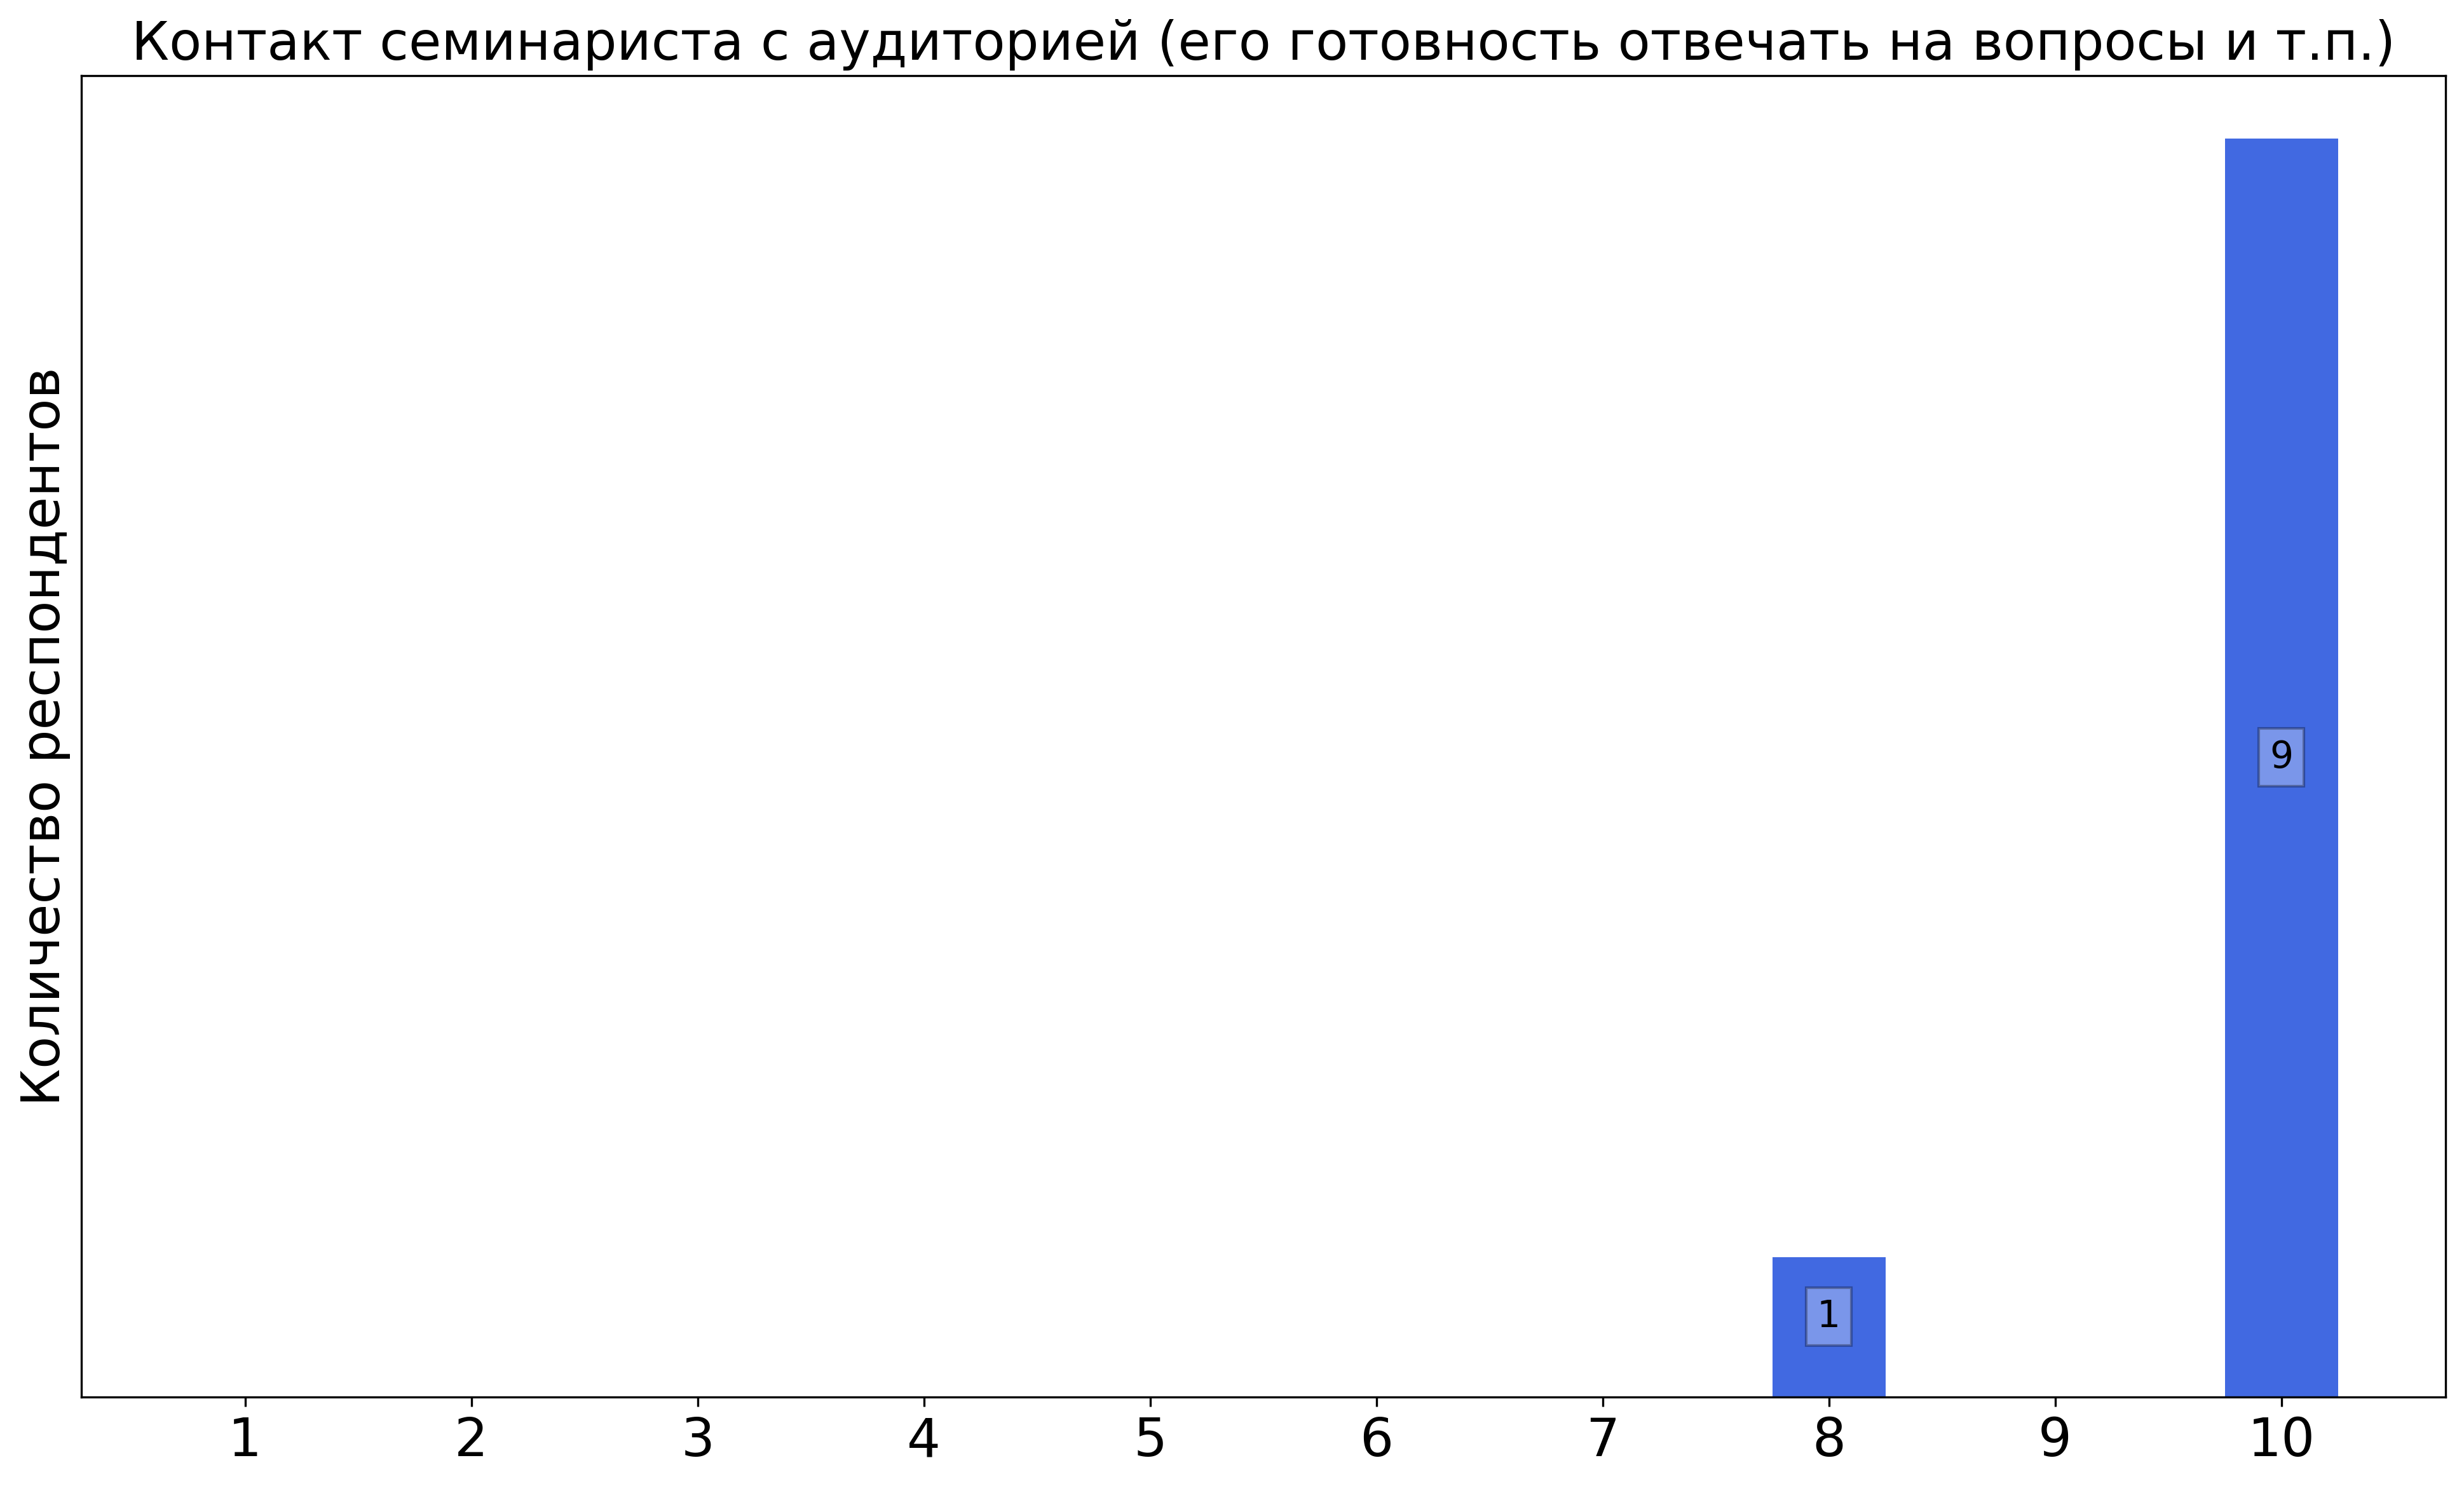
\includegraphics[width=\textwidth]{images/1 course/Информатика/seminarists-marks-Винокуров Н.А.-0.png}
            \end{subfigure}
            \begin{subfigure}[b]{0.45\textwidth}
                \centering
                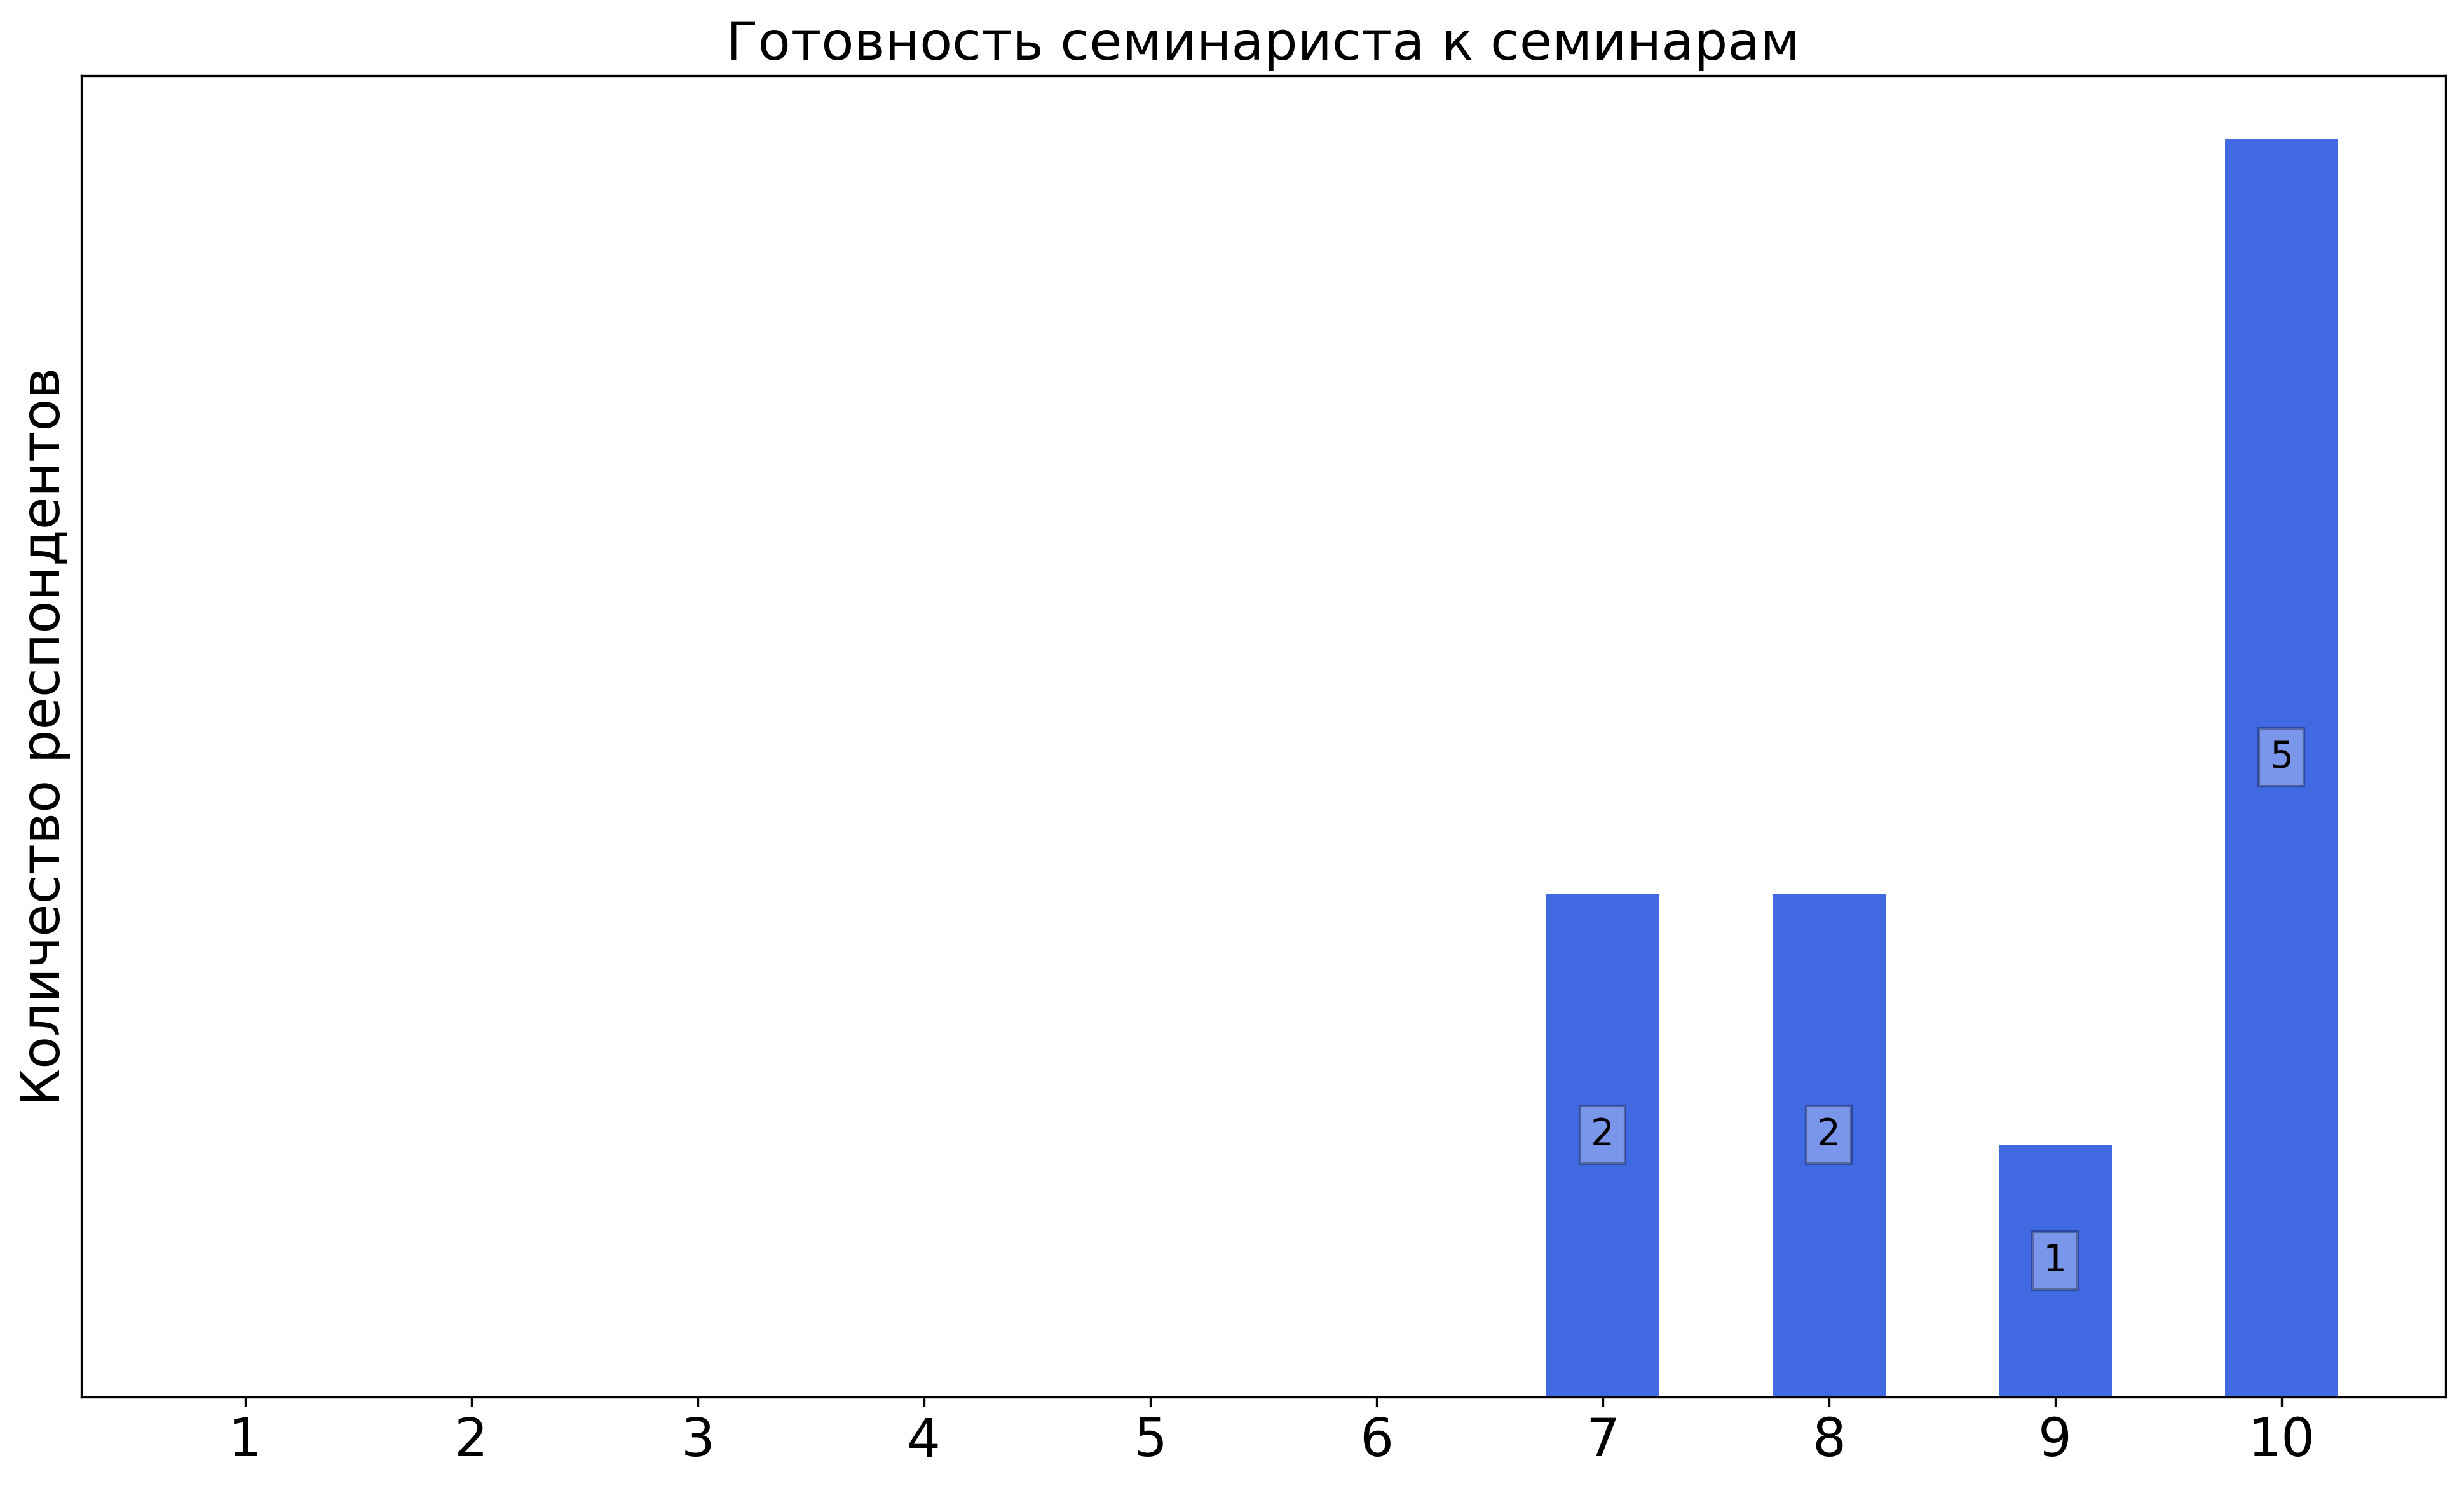
\includegraphics[width=\textwidth]{images/1 course/Информатика/seminarists-marks-Винокуров Н.А.-1.png}
            \end{subfigure}
            \begin{subfigure}[b]{0.45\textwidth}
                \centering
                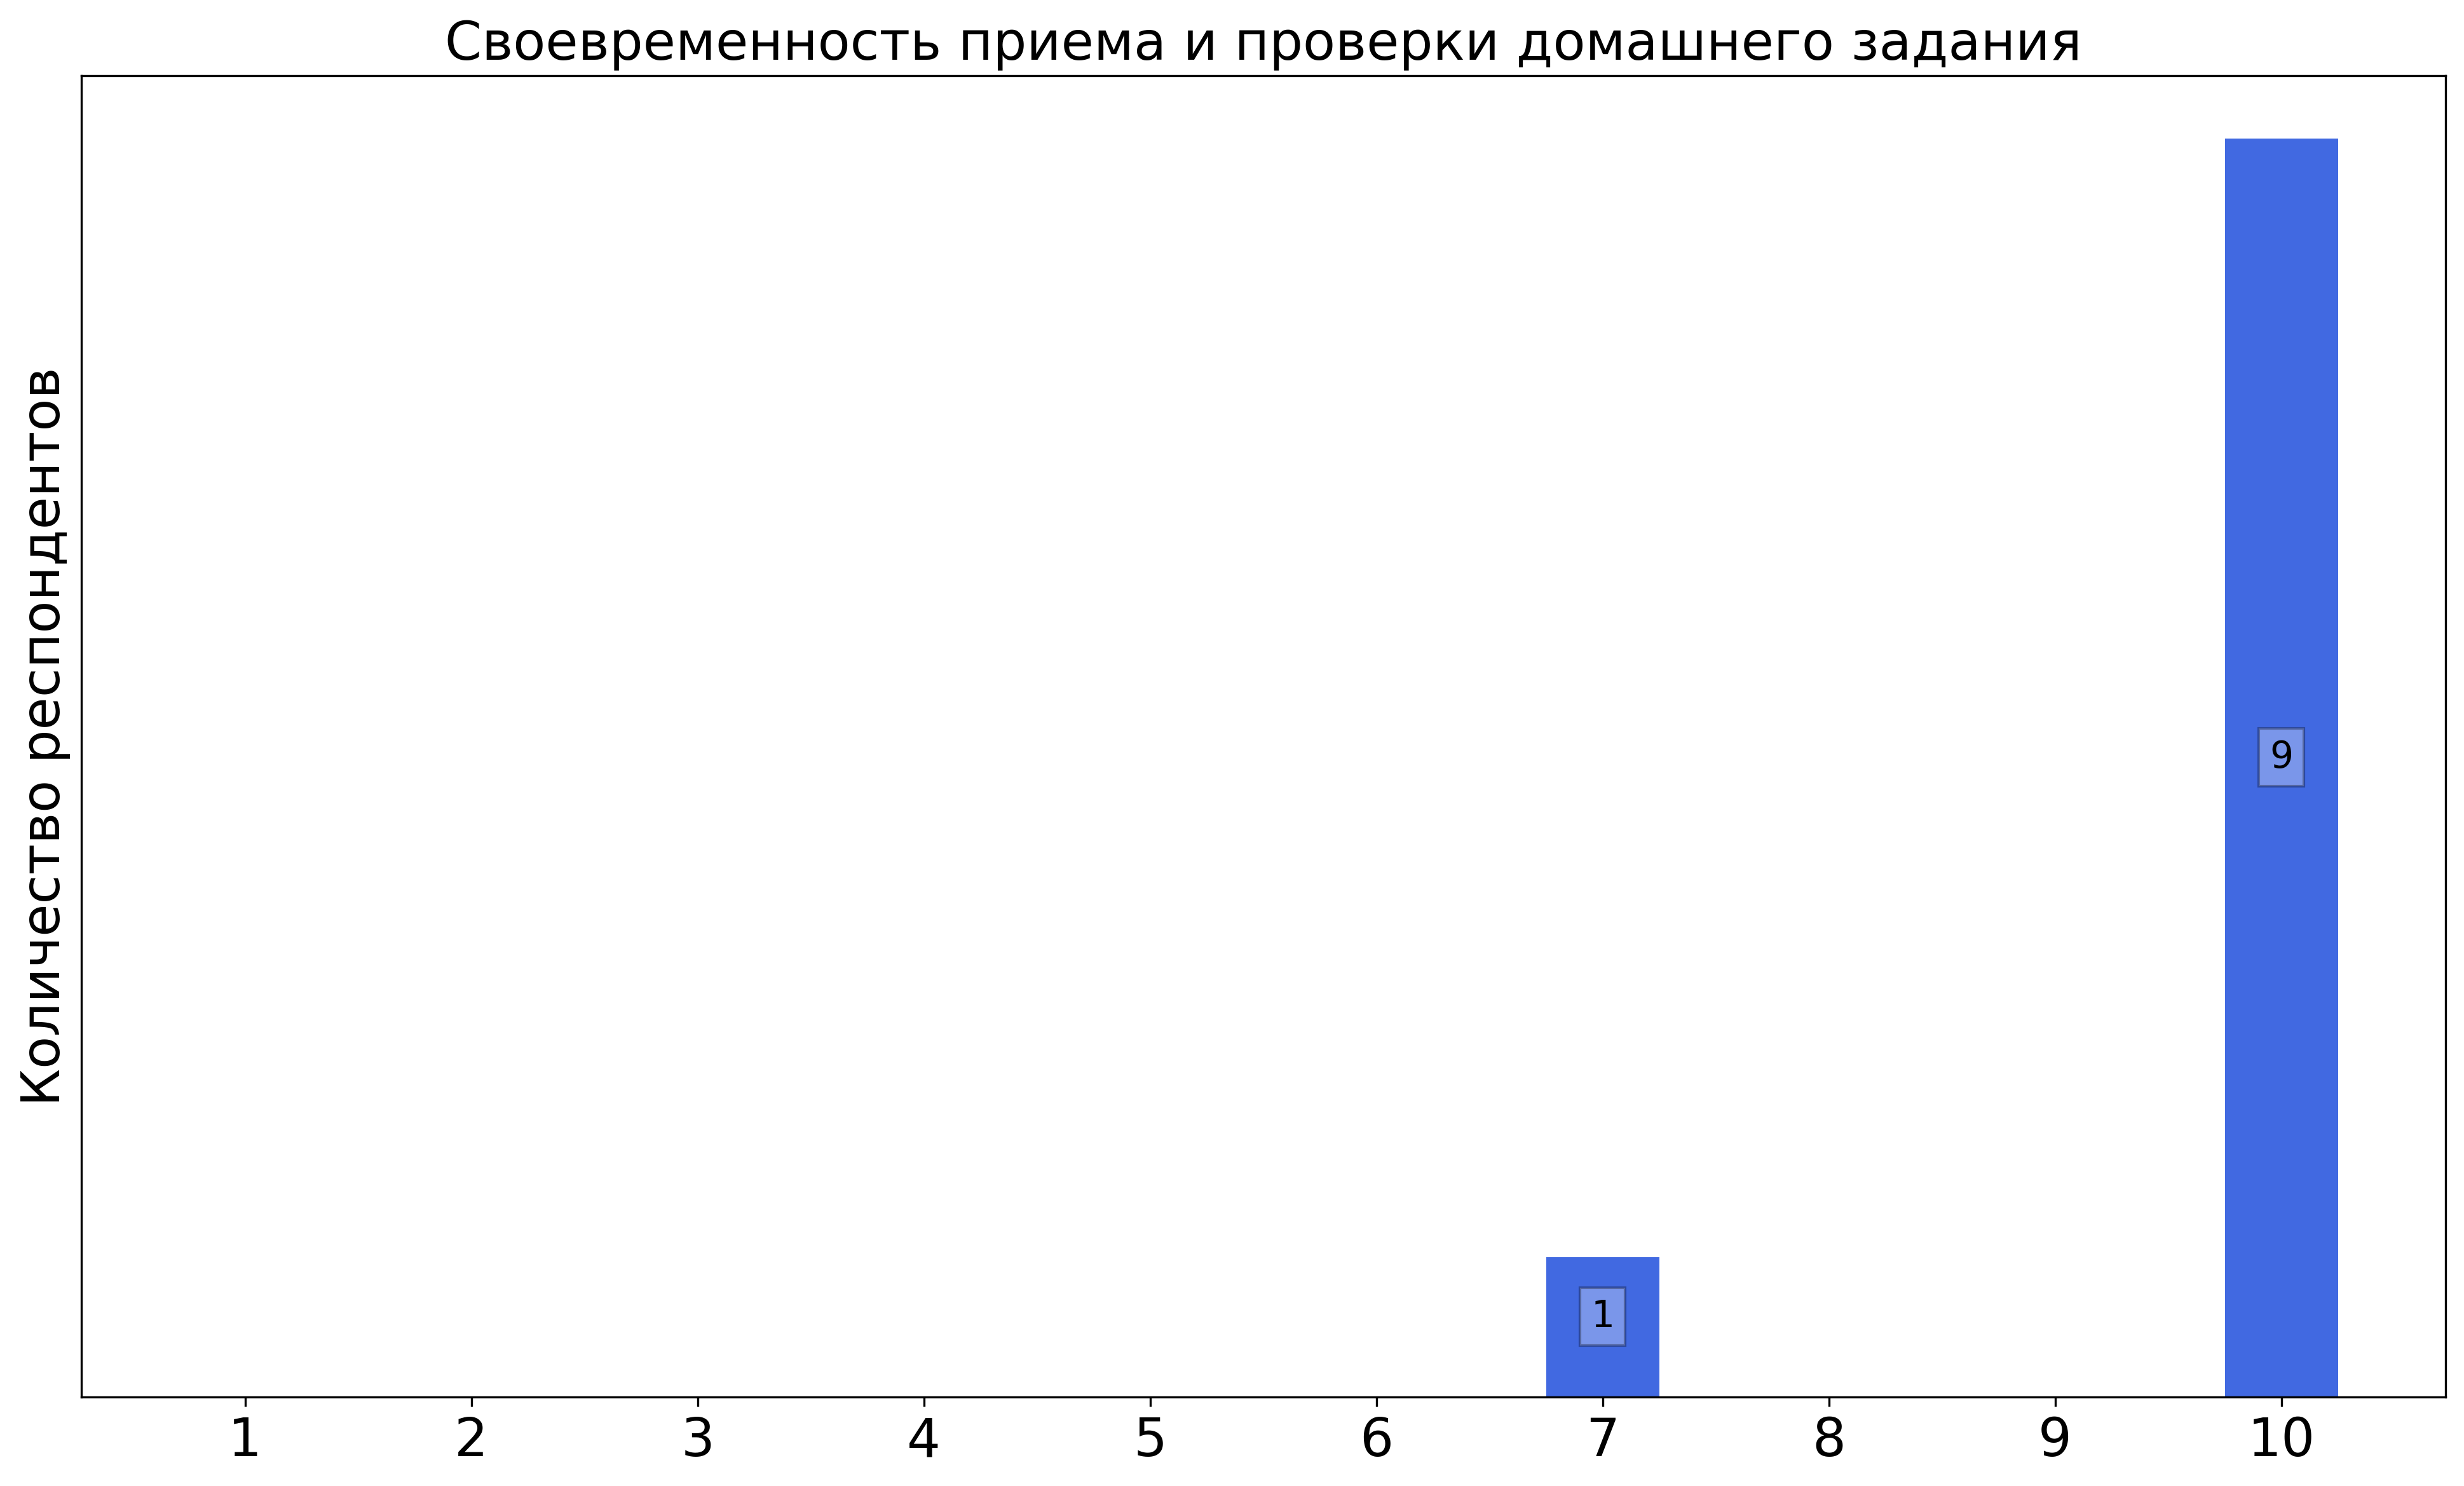
\includegraphics[width=\textwidth]{images/1 course/Информатика/seminarists-marks-Винокуров Н.А.-2.png}
            \end{subfigure}
            \begin{subfigure}[b]{0.45\textwidth}
                \centering
                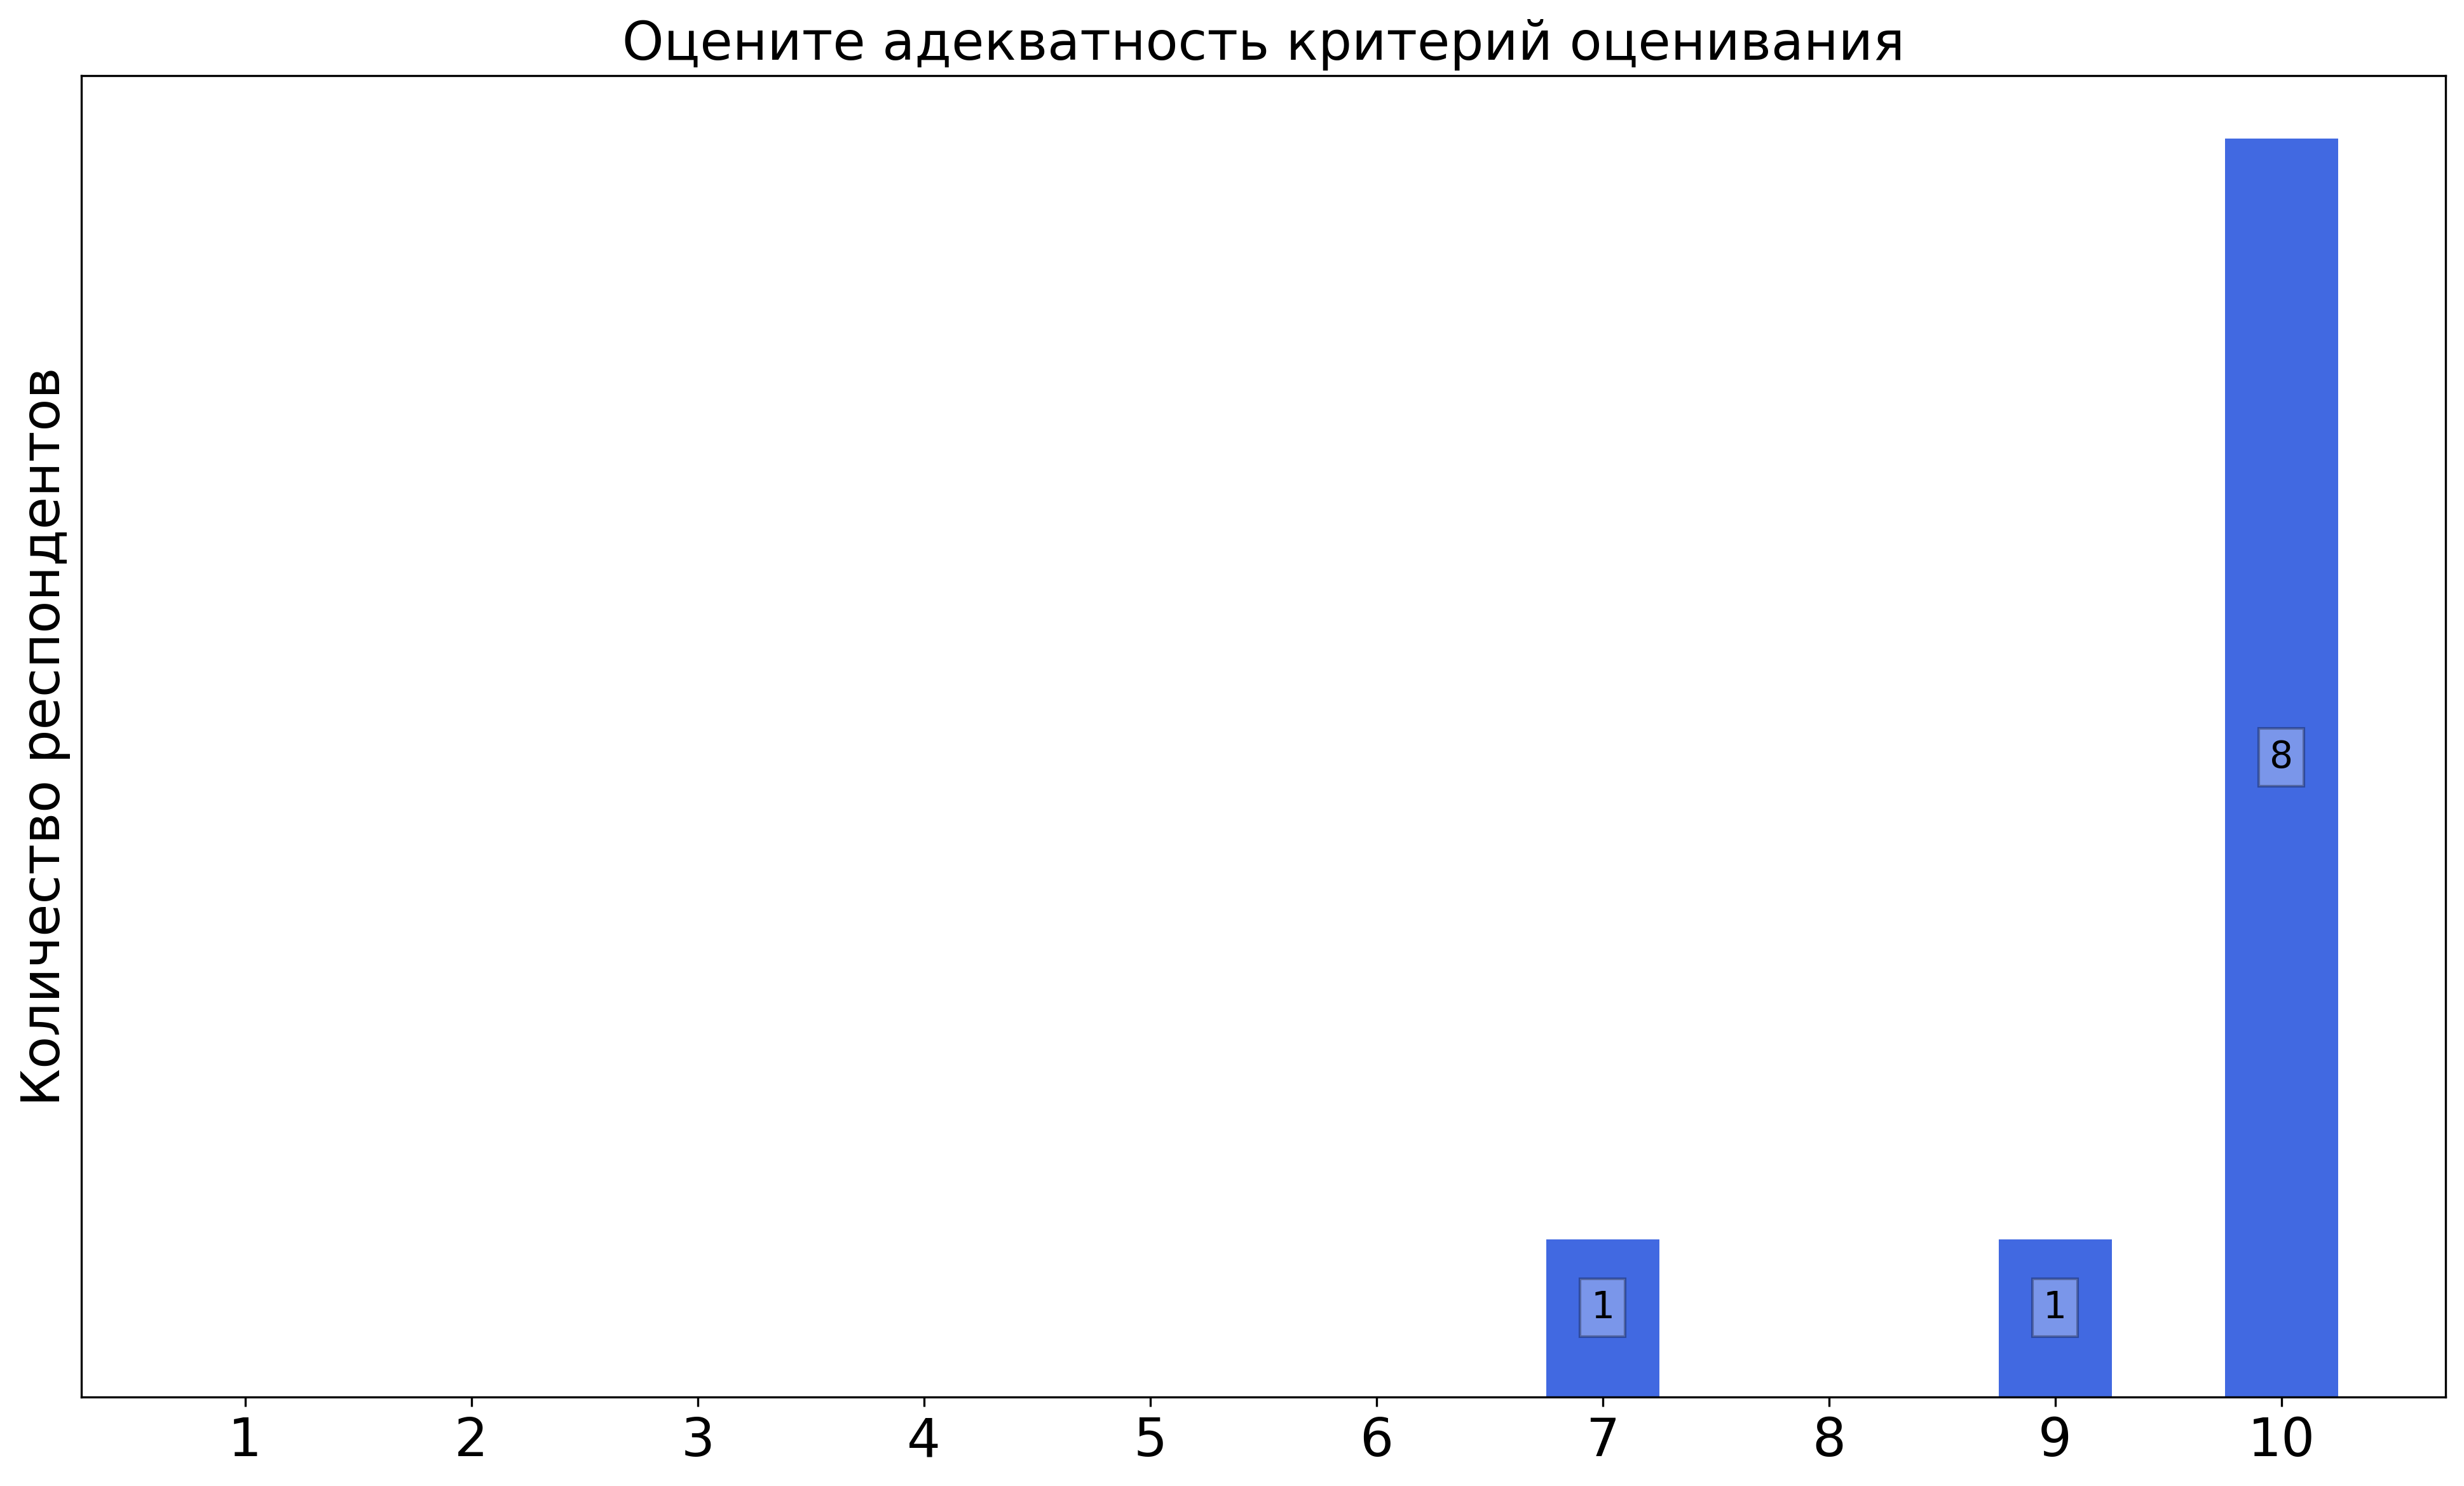
\includegraphics[width=\textwidth]{images/1 course/Информатика/seminarists-marks-Винокуров Н.А.-3.png}
            \end{subfigure}	
            \caption{Оценки респондентов о качестве преподавания семинаров}
        \end{figure}

        \textbf{Комментарии студентов о семинаристе\protect\footnote{сохранены оригинальные орфография и пунктуация}}
            \begin{commentbox} 
                Лучший семинарист, правда хорошо все объясняет и учит быстро и лаконично писать код (ну очев, он же  lisp guy). Благодаря нему узнал про много структур данных, которые например дед на хуавее не дает. В свободное время всегда готов проконсультировать и помочь вам в написании кода. 
            \end{commentbox} 
        
            \begin{commentbox} 
                Замечательный преподаватель. Объясняет все очень хорошо, иногда не все понятно, но охотно отвечает на вопросы. Очень хорошо разбирается в программировании, может научить многому, если студент сам захочет. Оценки ставит очень лояльно, никому ниже хор5 не поставил. 
            \end{commentbox} 
        
            \begin{commentbox} 
                В школе я недолюбливал информатику. Большое спасибо Никите Алексеевичу - привил интерес (наряду с Ильёй Рудольфовичем)! Материала на семинаре много, материал увлекает; на занятии не успеваю за Никитой Алексеевичем, программирую после семинара. 
            \end{commentbox} 
        
            \begin{commentbox} 
                отличный семинарист 
            \end{commentbox} 
        
            \begin{commentbox} 
                Приятен в общении и всегда готов помочь даже с самой глупой проблемой. На семинарах объясние достаточно сложные темы, но понятным языком 
            \end{commentbox} 
        
            \begin{commentbox} 
                Часто уходит от программы и рассказывает интересные темы. Для тех, у кого есть опыт или занимается на доп курсах (хуавей или айлаб) просто отлично (как мне, например), но тем, у кого знаний не так много, будет тяжело. Если ходит чисто к нему, то чего-то систематического и равномерного лучше не ожидать 
            \end{commentbox} 

    
    \subsubsection{Отзыв студентов о семинарах. Семинарист: Дербышева Т.А.}
        \begin{figure}[H]
            \centering
            \begin{subfigure}[b]{0.45\textwidth}
                \centering
                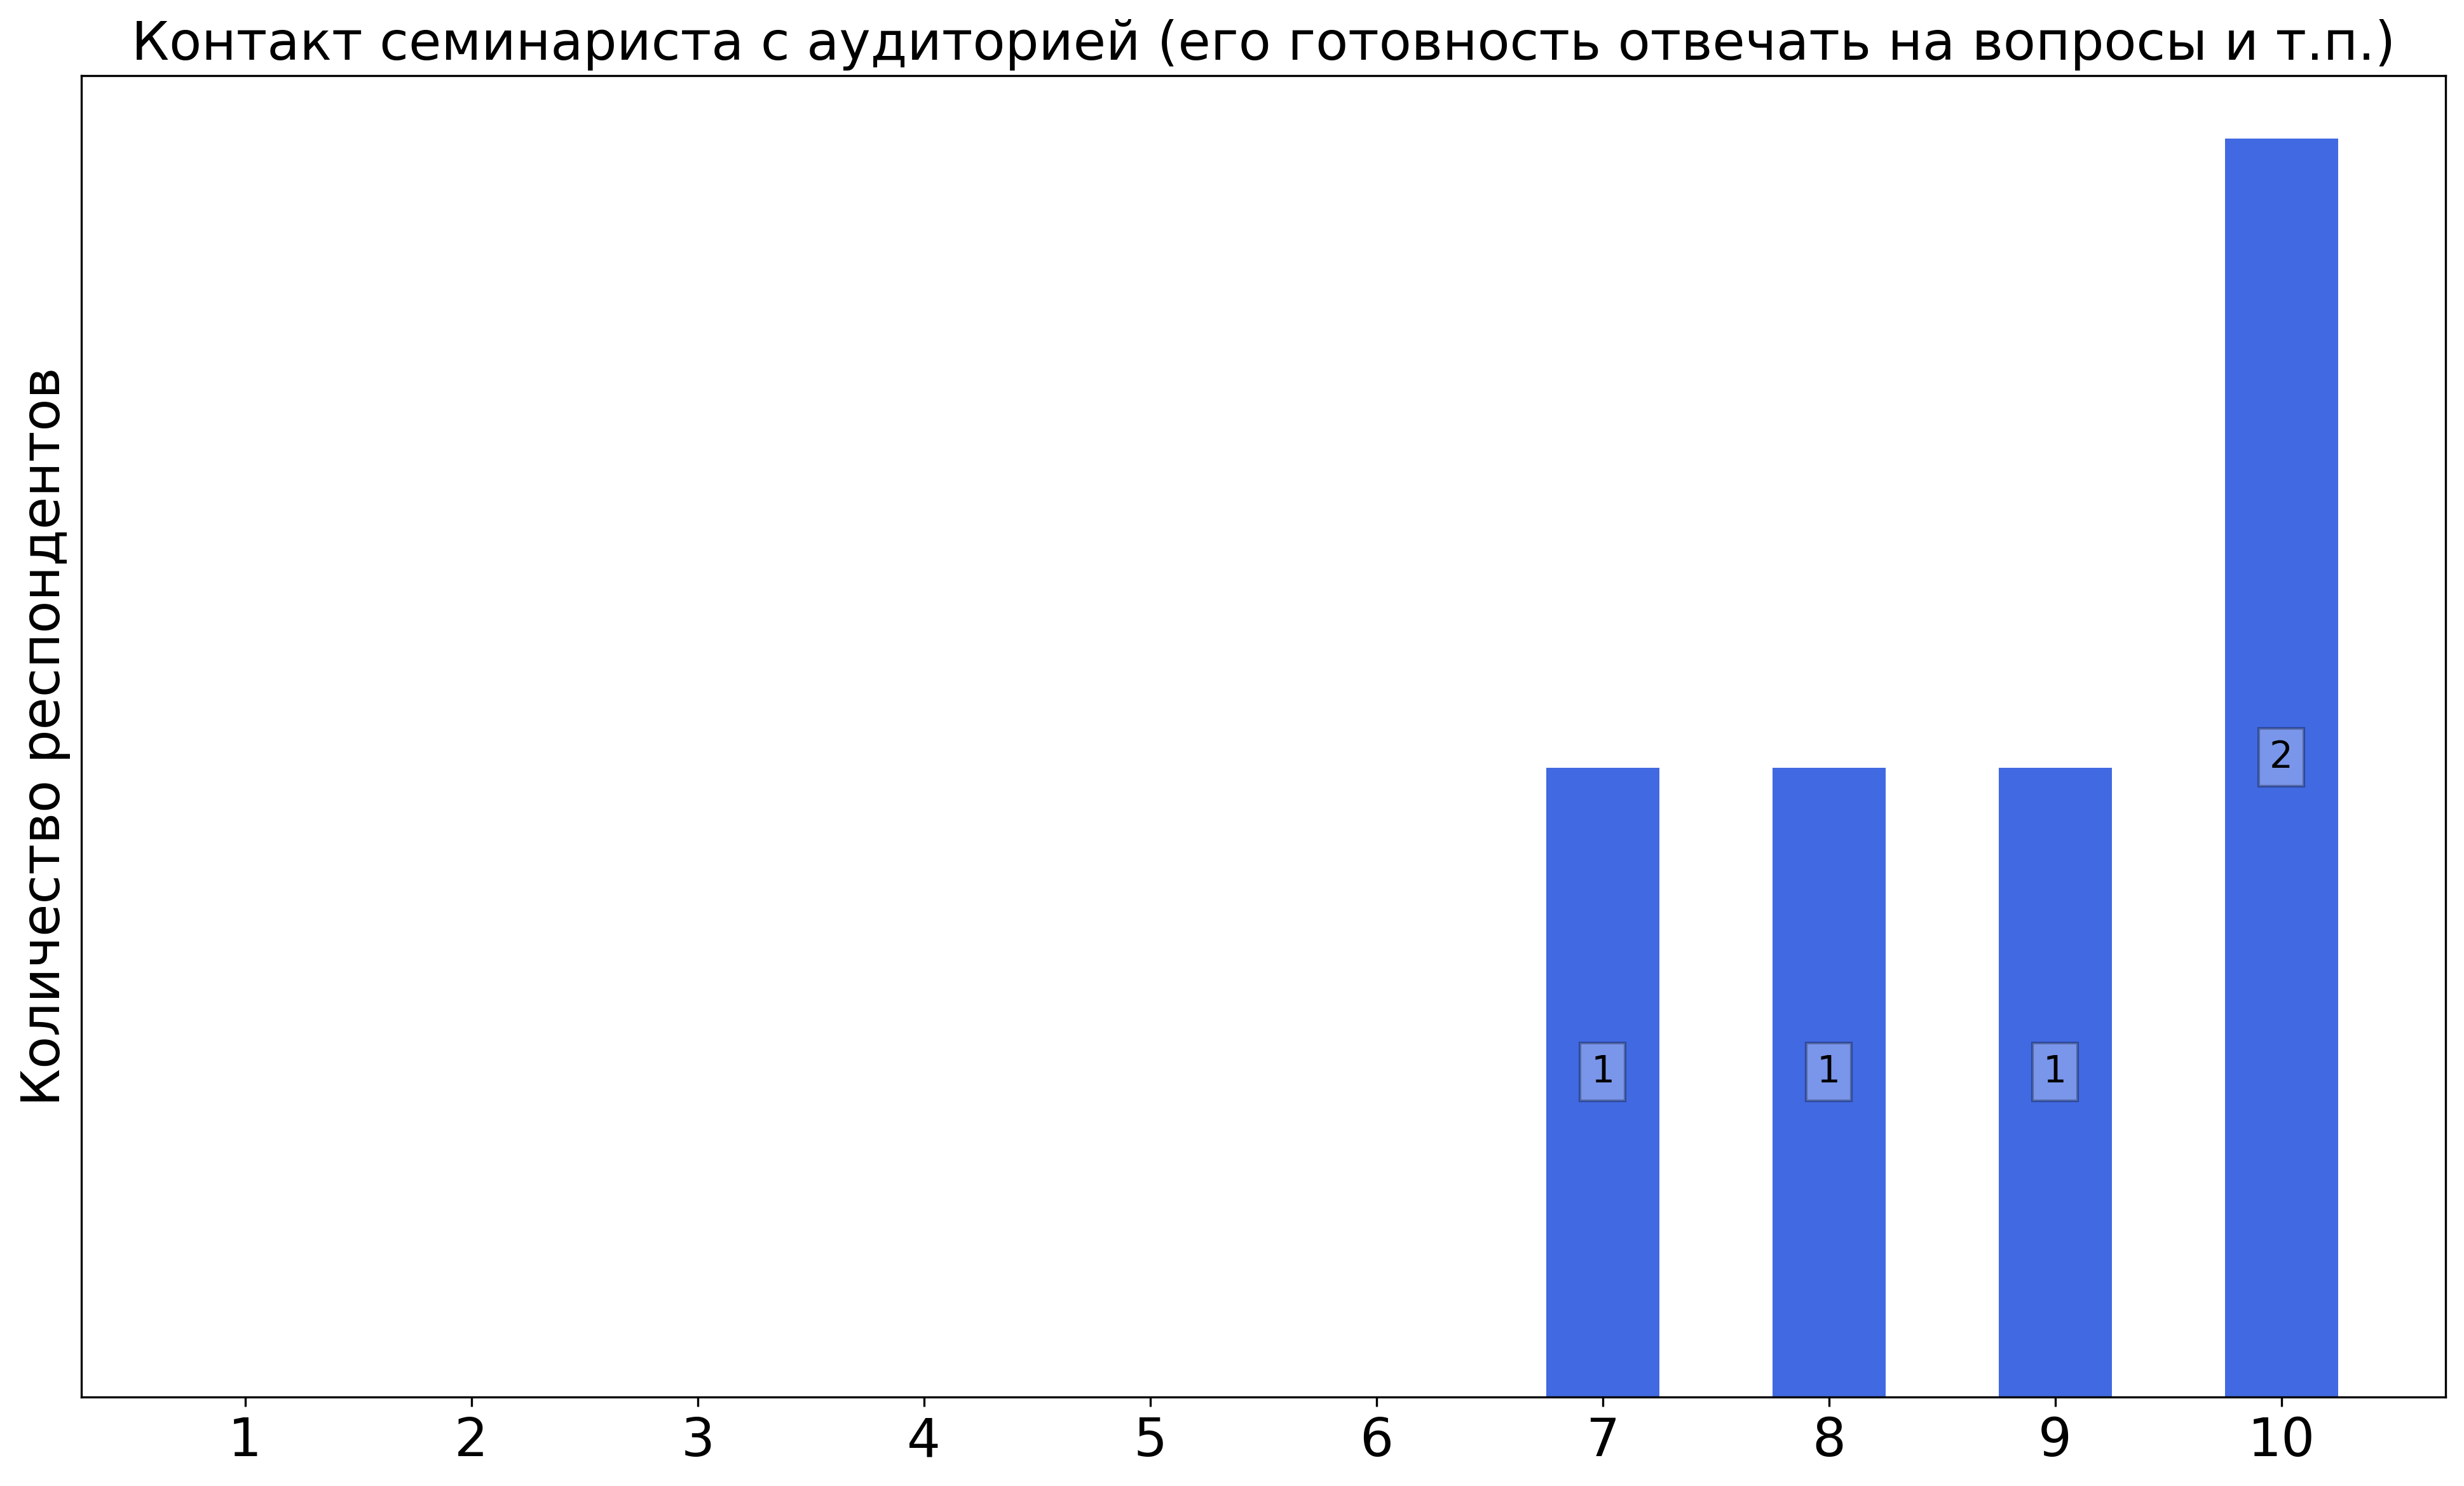
\includegraphics[width=\textwidth]{images/1 course/Информатика/seminarists-marks-Дербышева Т.А.-0.png}
            \end{subfigure}
            \begin{subfigure}[b]{0.45\textwidth}
                \centering
                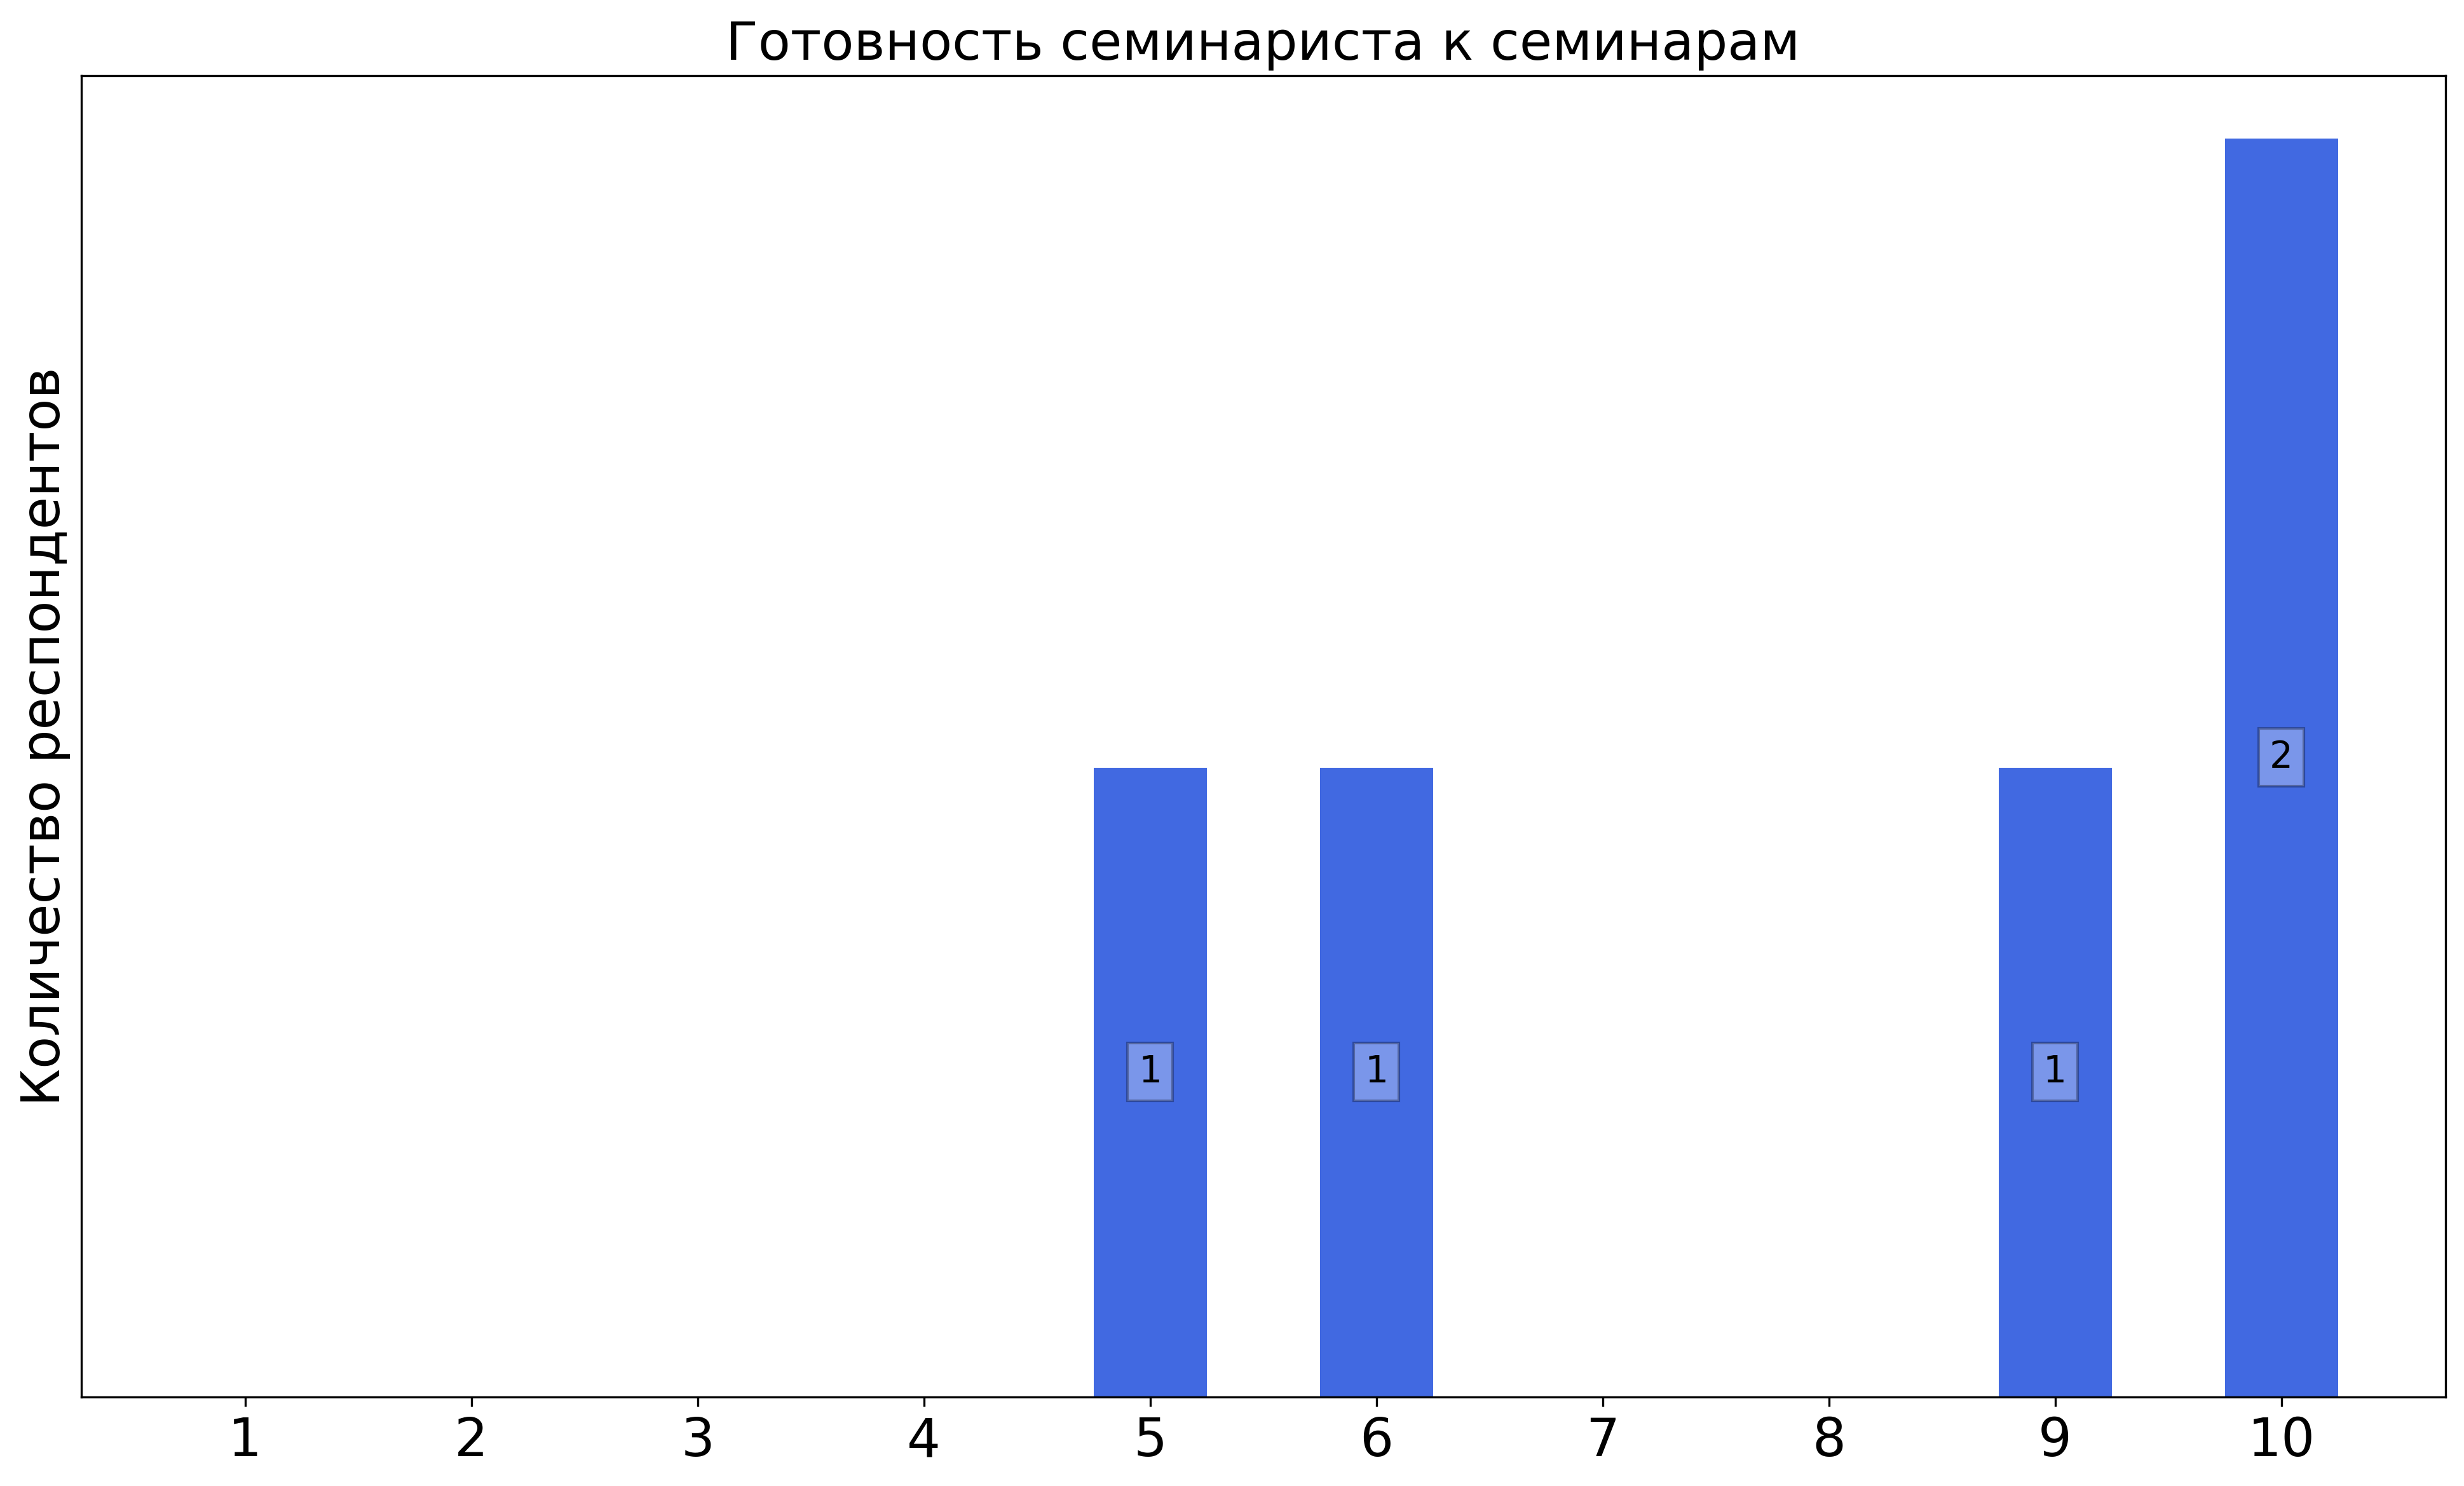
\includegraphics[width=\textwidth]{images/1 course/Информатика/seminarists-marks-Дербышева Т.А.-1.png}
            \end{subfigure}
            \begin{subfigure}[b]{0.45\textwidth}
                \centering
                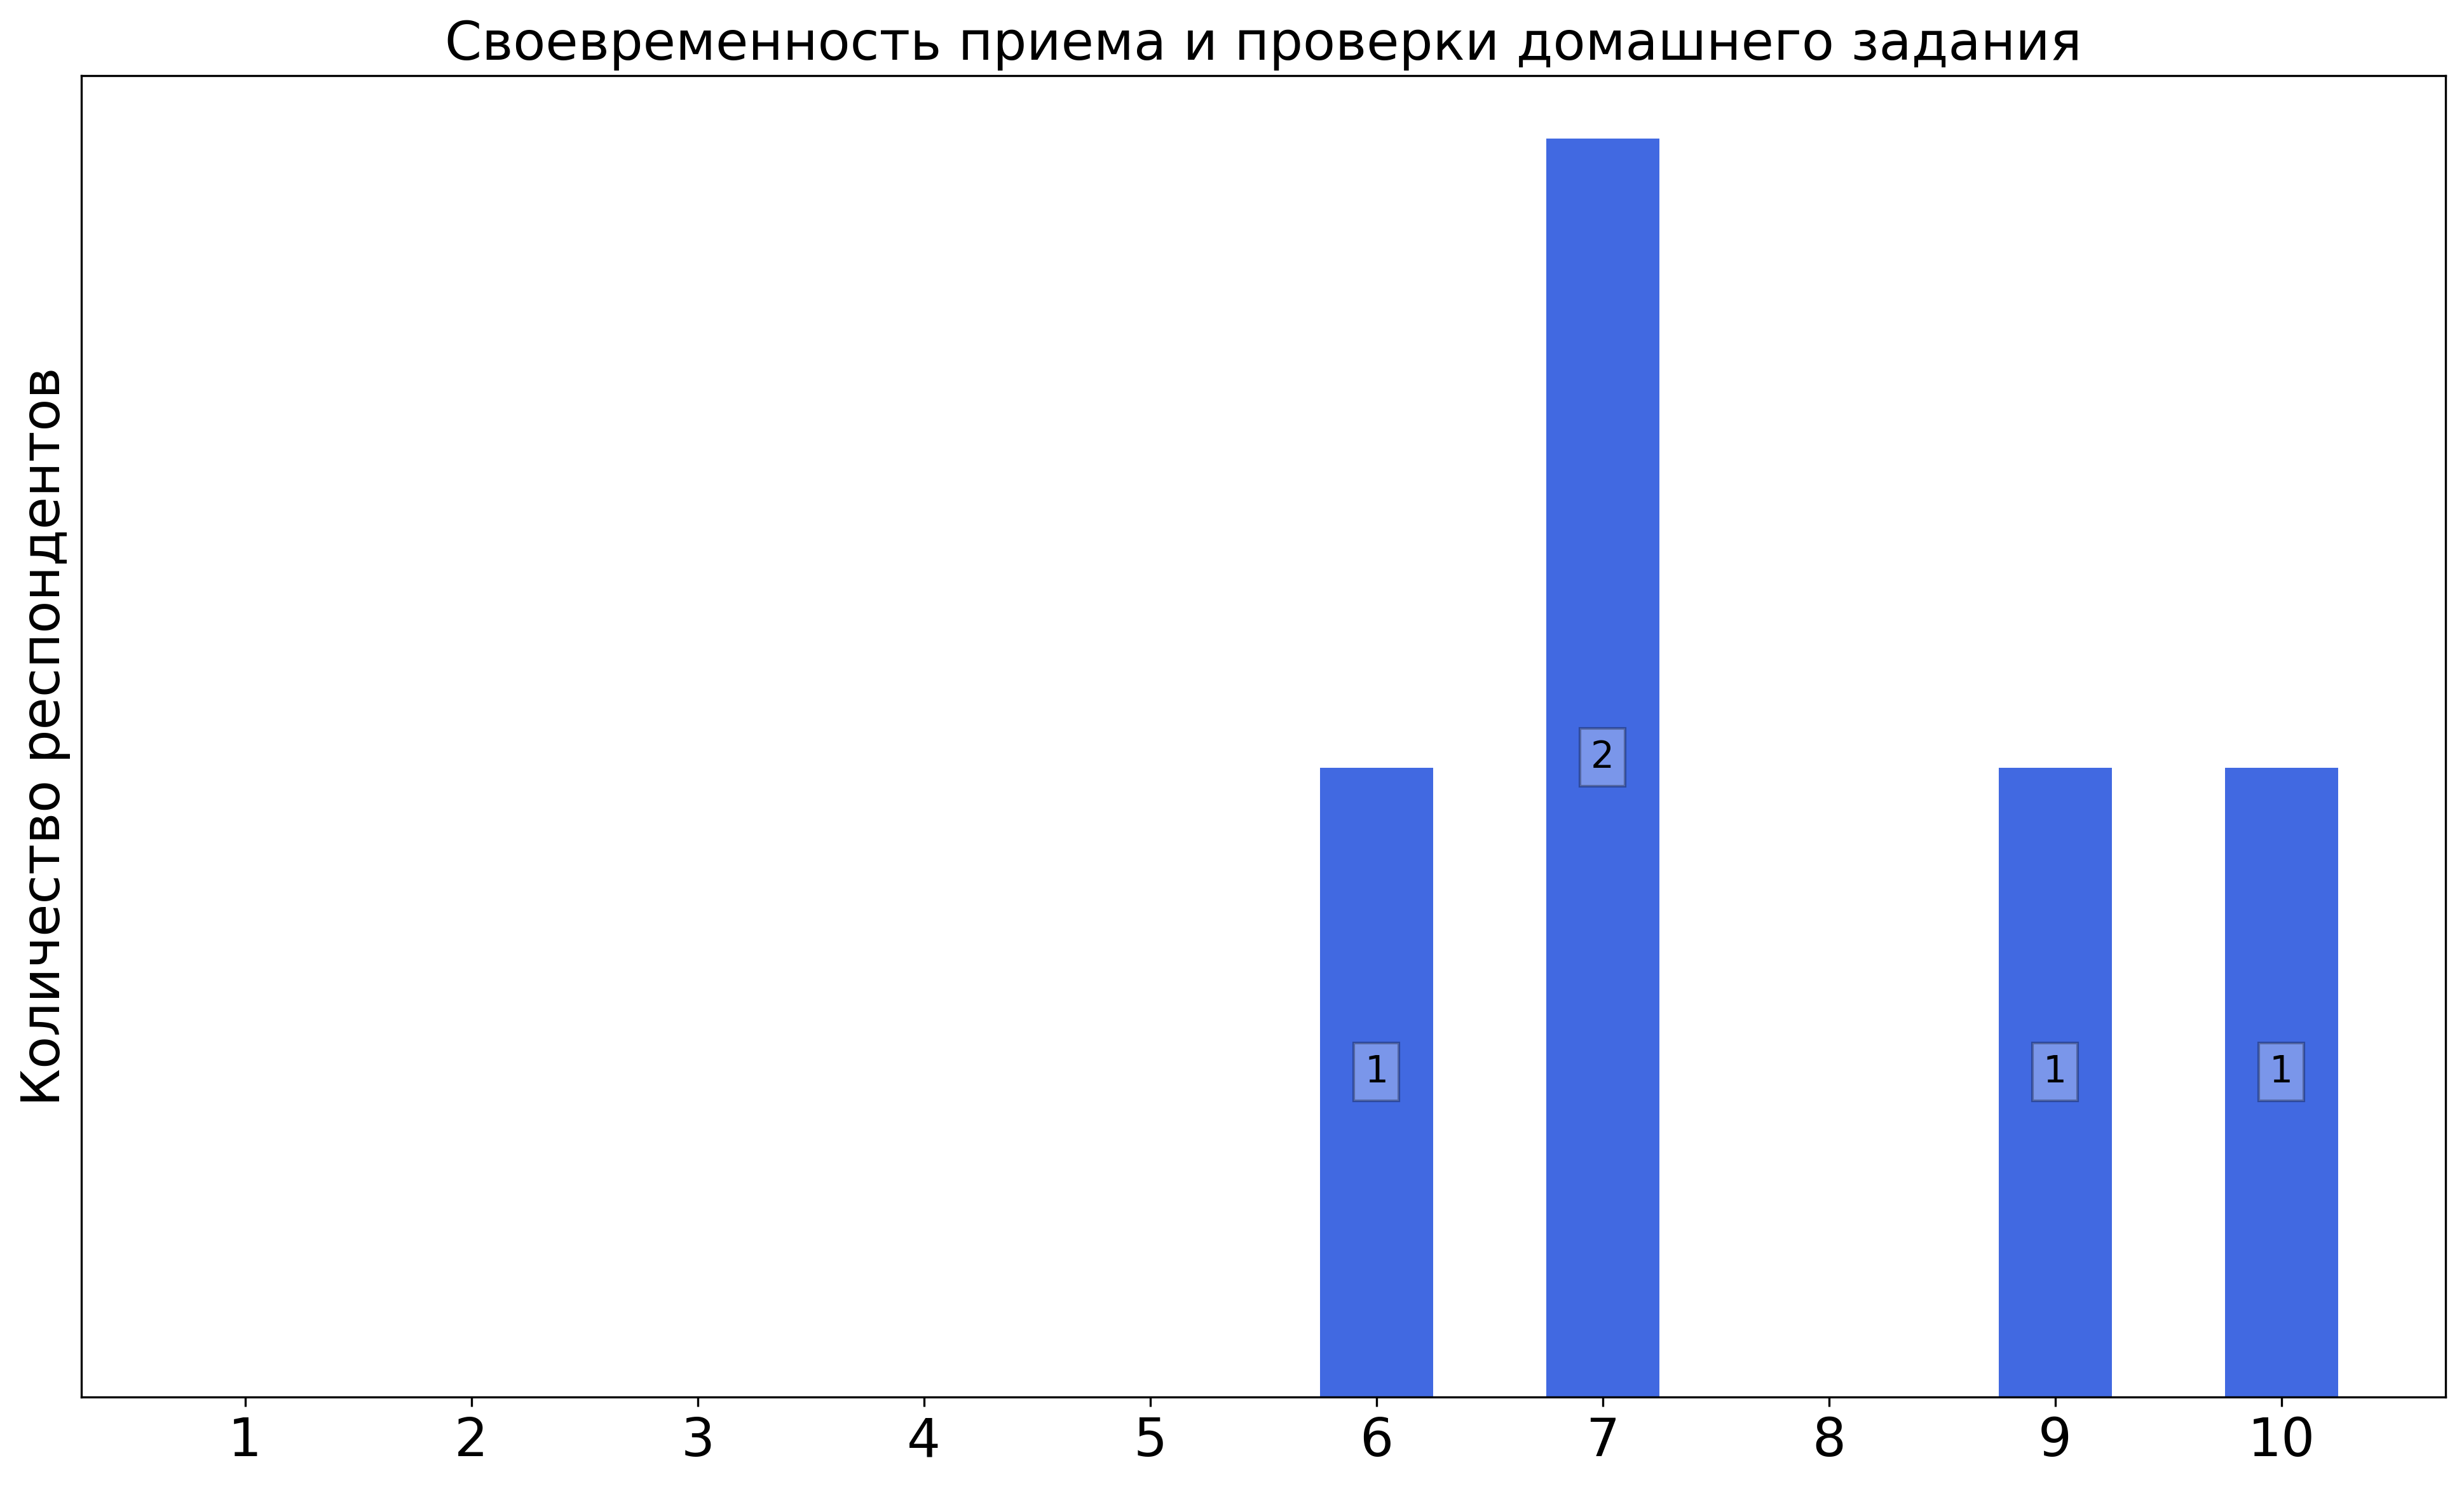
\includegraphics[width=\textwidth]{images/1 course/Информатика/seminarists-marks-Дербышева Т.А.-2.png}
            \end{subfigure}
            \begin{subfigure}[b]{0.45\textwidth}
                \centering
                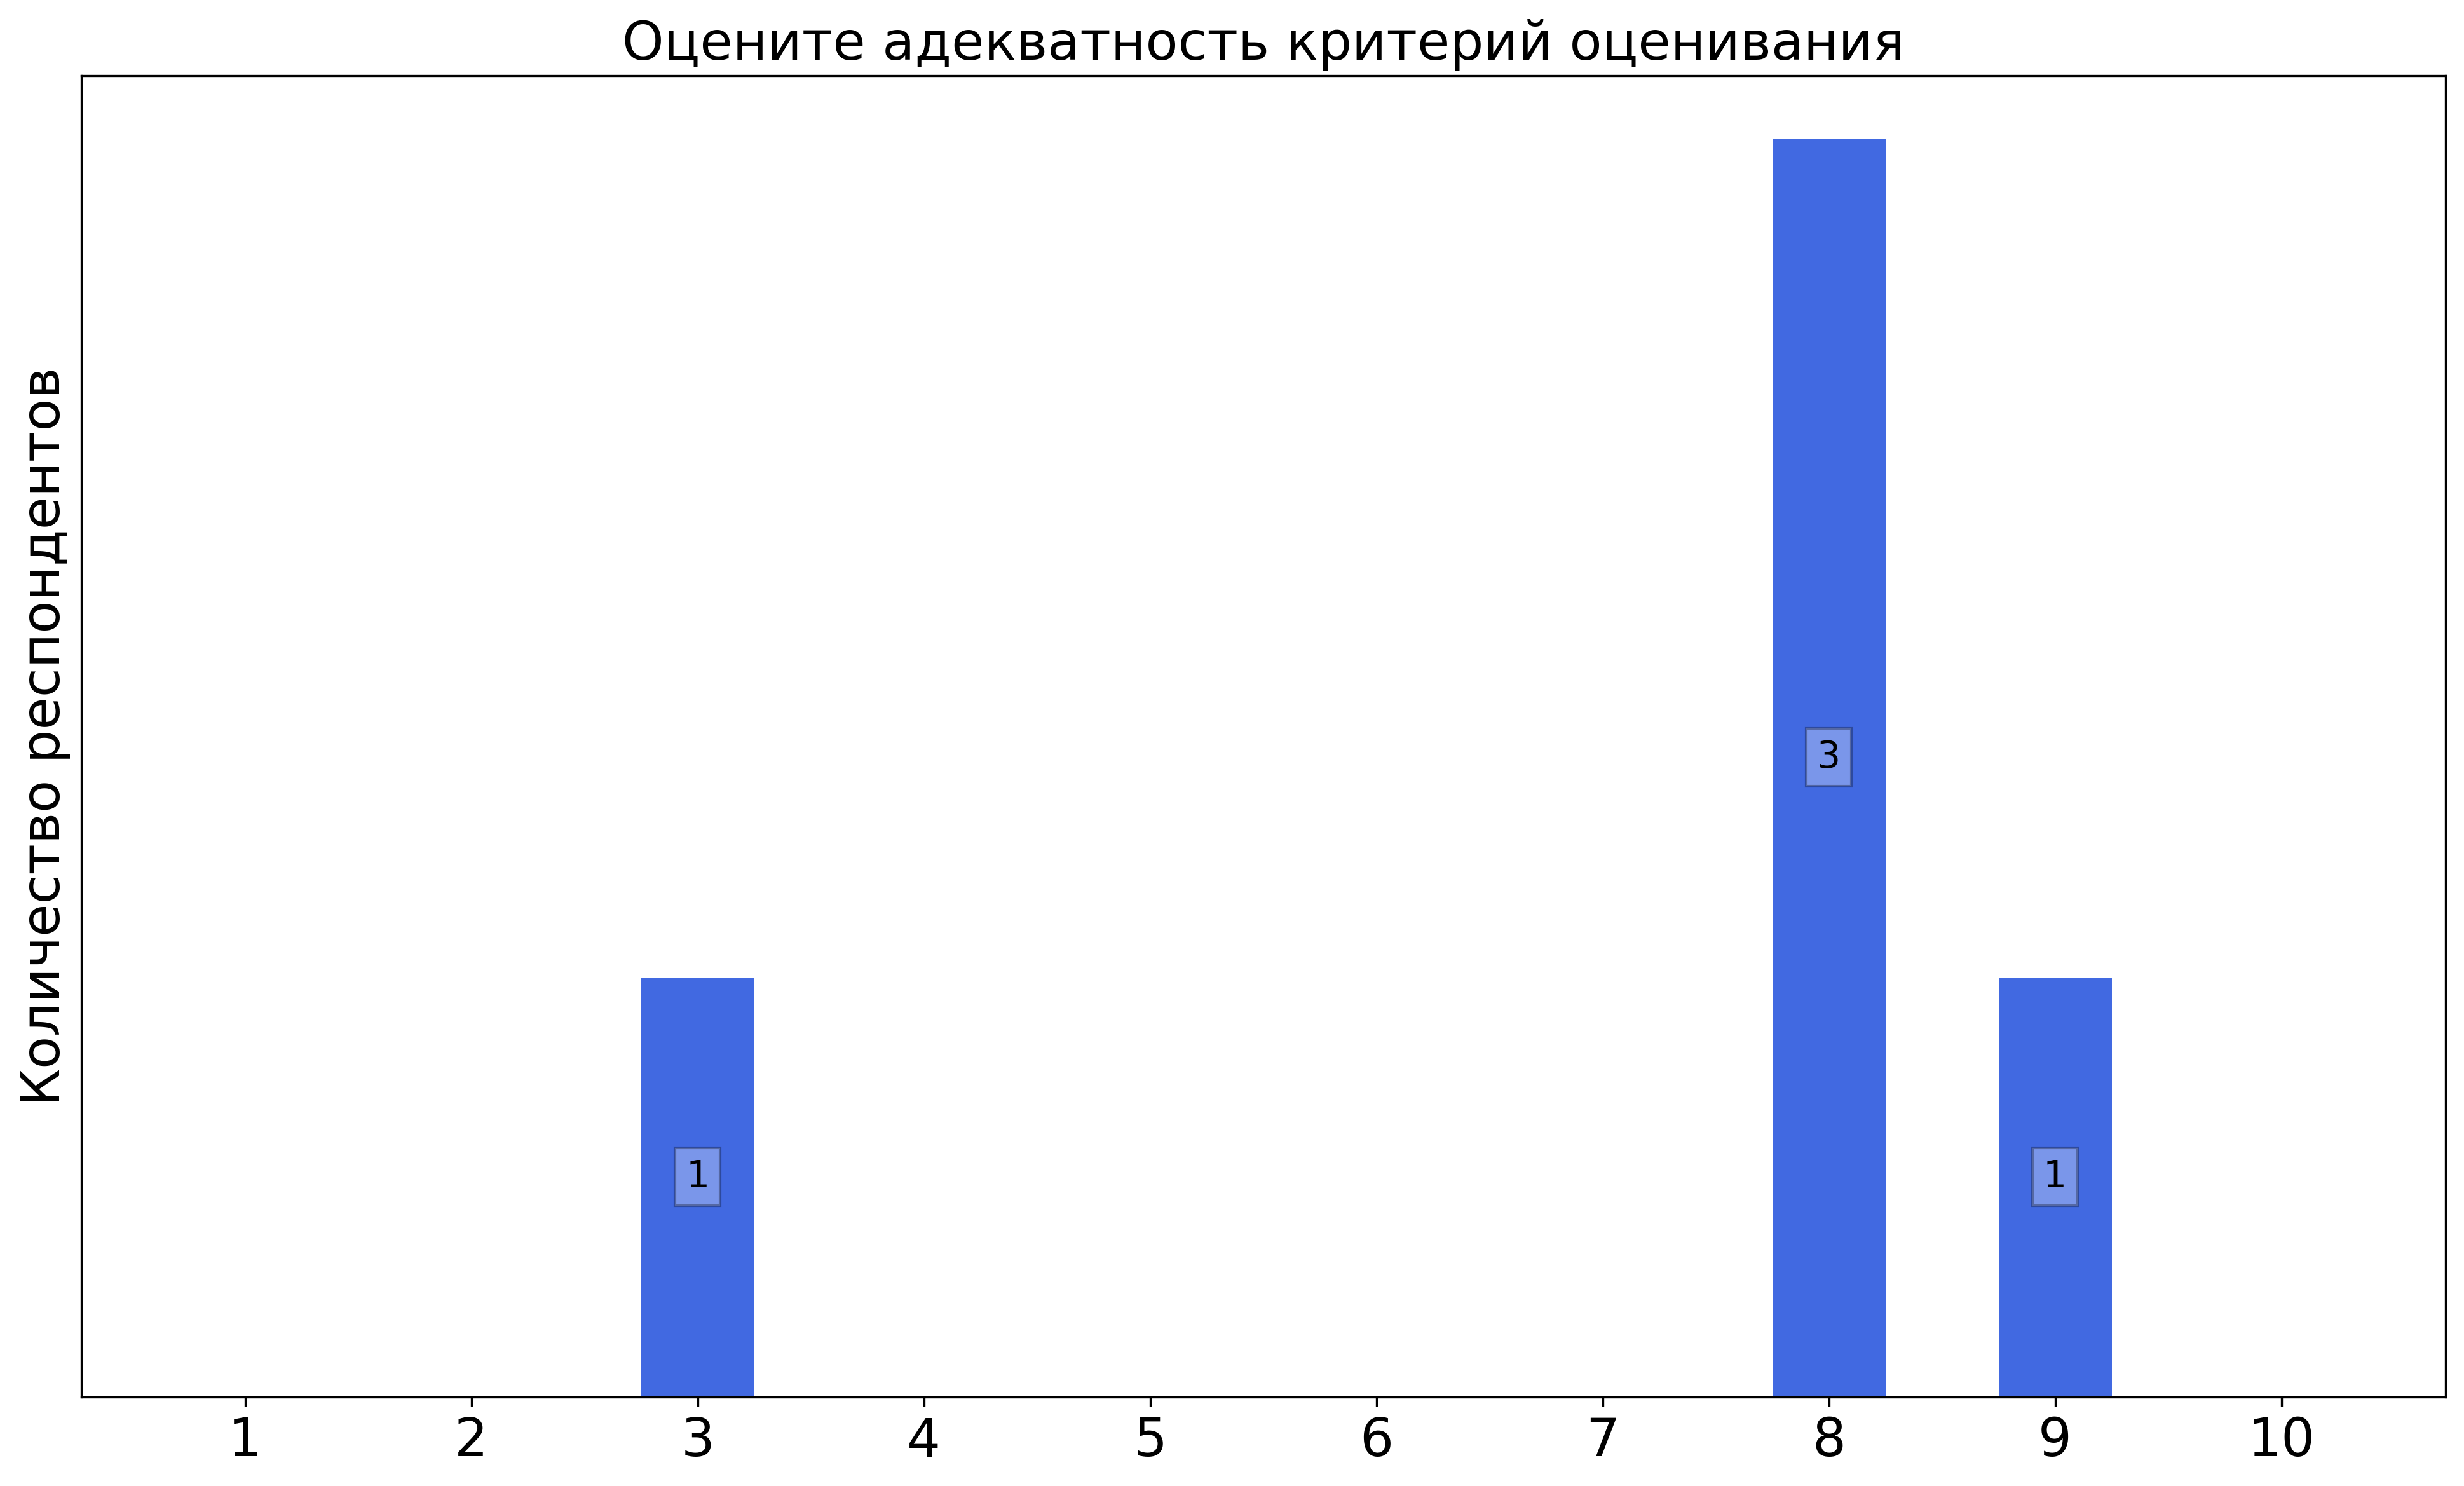
\includegraphics[width=\textwidth]{images/1 course/Информатика/seminarists-marks-Дербышева Т.А.-3.png}
            \end{subfigure}	
            \caption{Оценки респондентов о качестве преподавания семинаров}
        \end{figure}

    
    \subsubsection{Отзыв студентов о семинарах. Семинарист: Хохлов В.К.}
		\begin{figure}[H]
			\centering
			\begin{subfigure}[b]{0.45\textwidth}
				\centering
				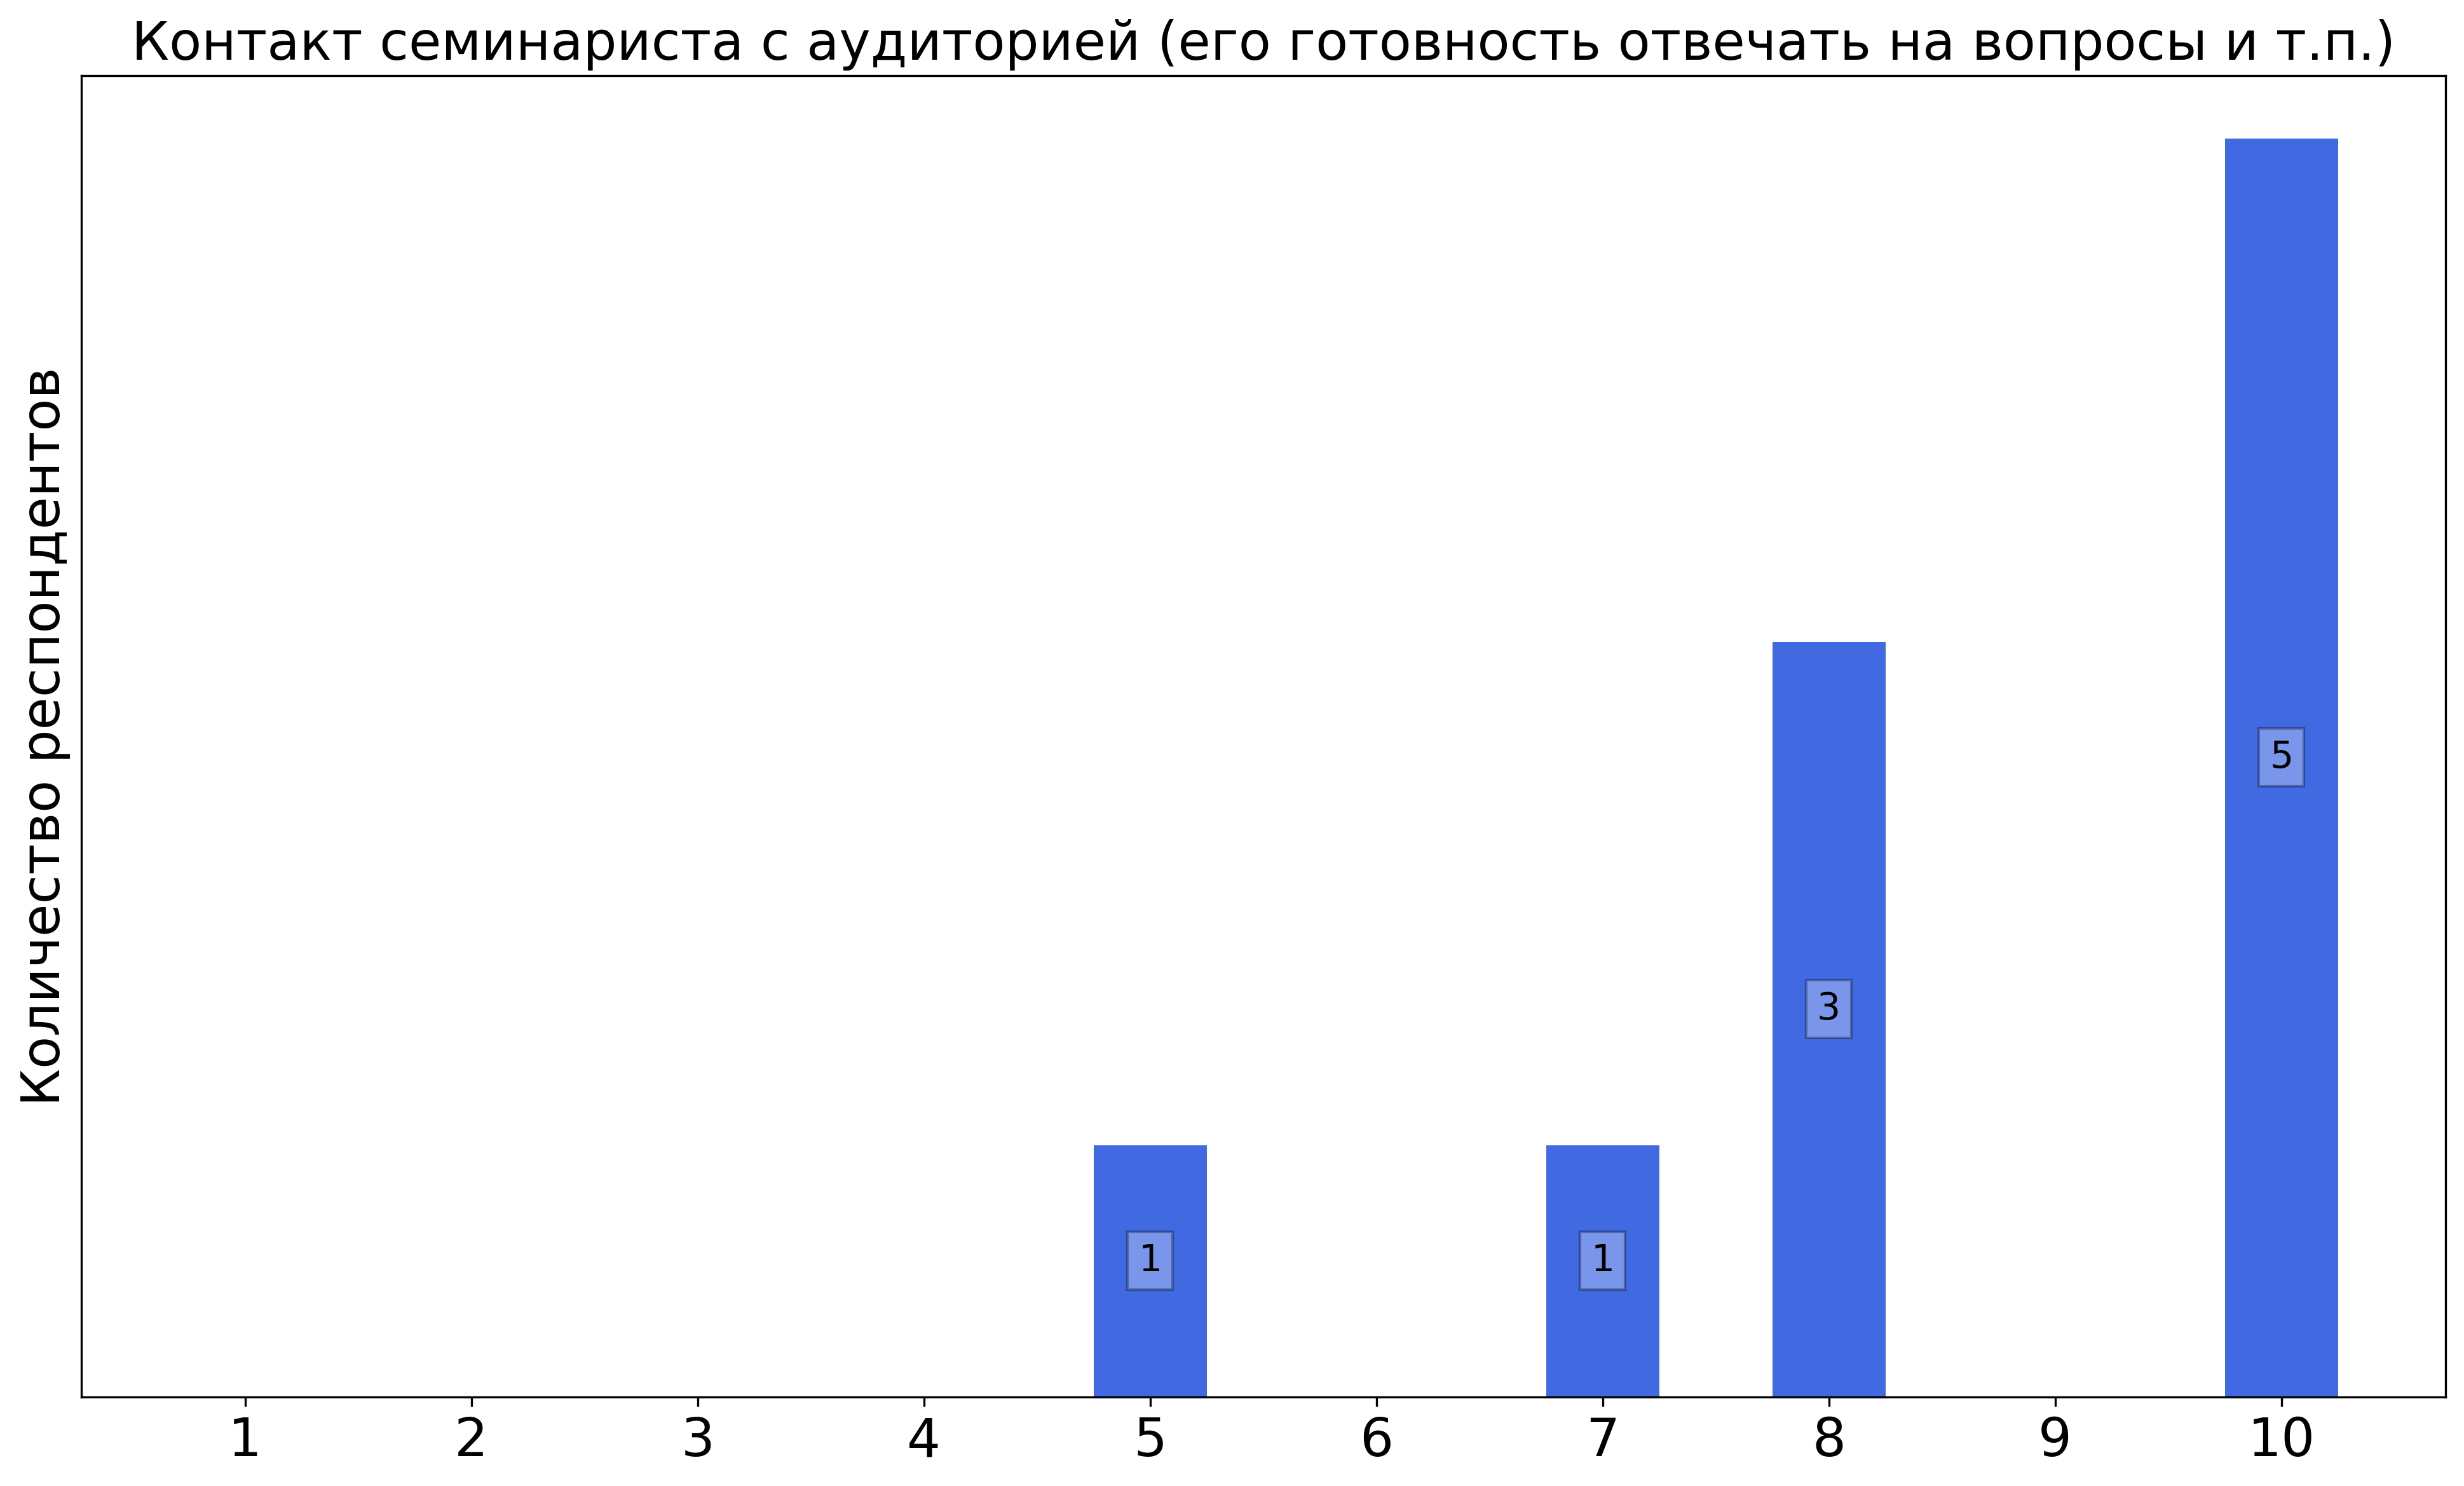
\includegraphics[width=\textwidth]{images/1 course/Информатика/seminarists-marks-Хохлов В.К.-0.png}
			\end{subfigure}
			\begin{subfigure}[b]{0.45\textwidth}
				\centering
				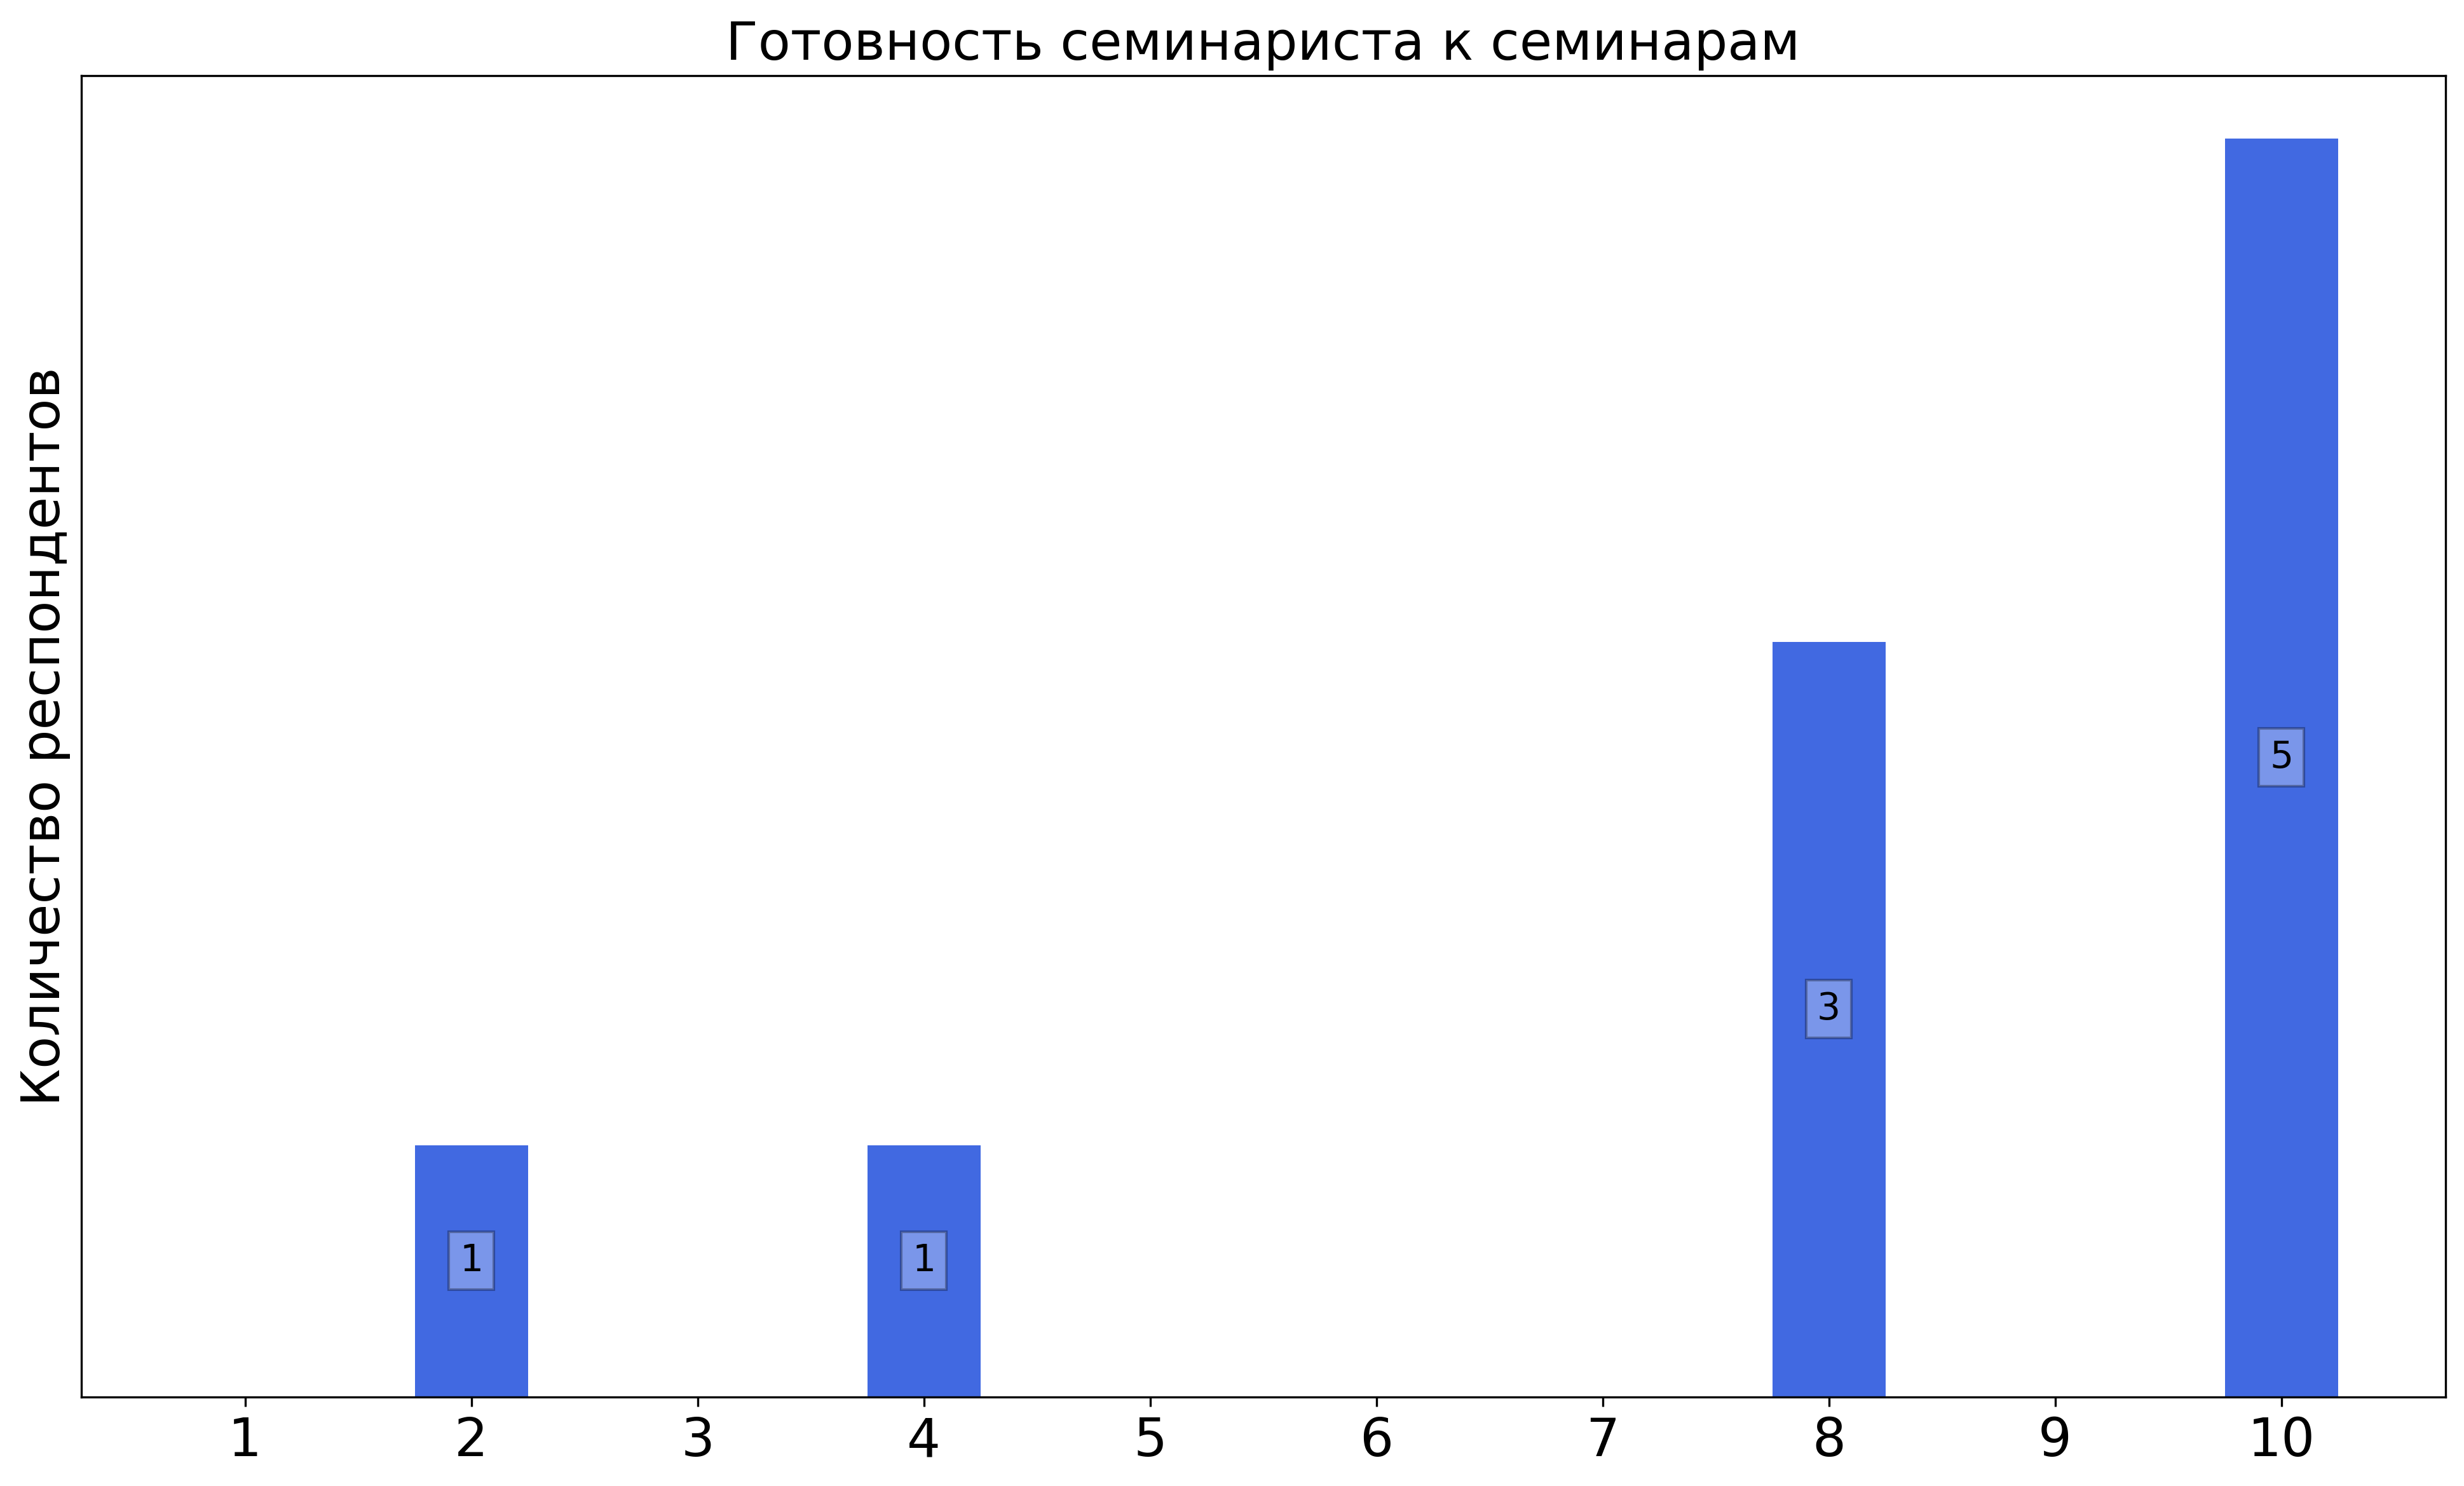
\includegraphics[width=\textwidth]{images/1 course/Информатика/seminarists-marks-Хохлов В.К.-1.png}
			\end{subfigure}
			\begin{subfigure}[b]{0.45\textwidth}
				\centering
				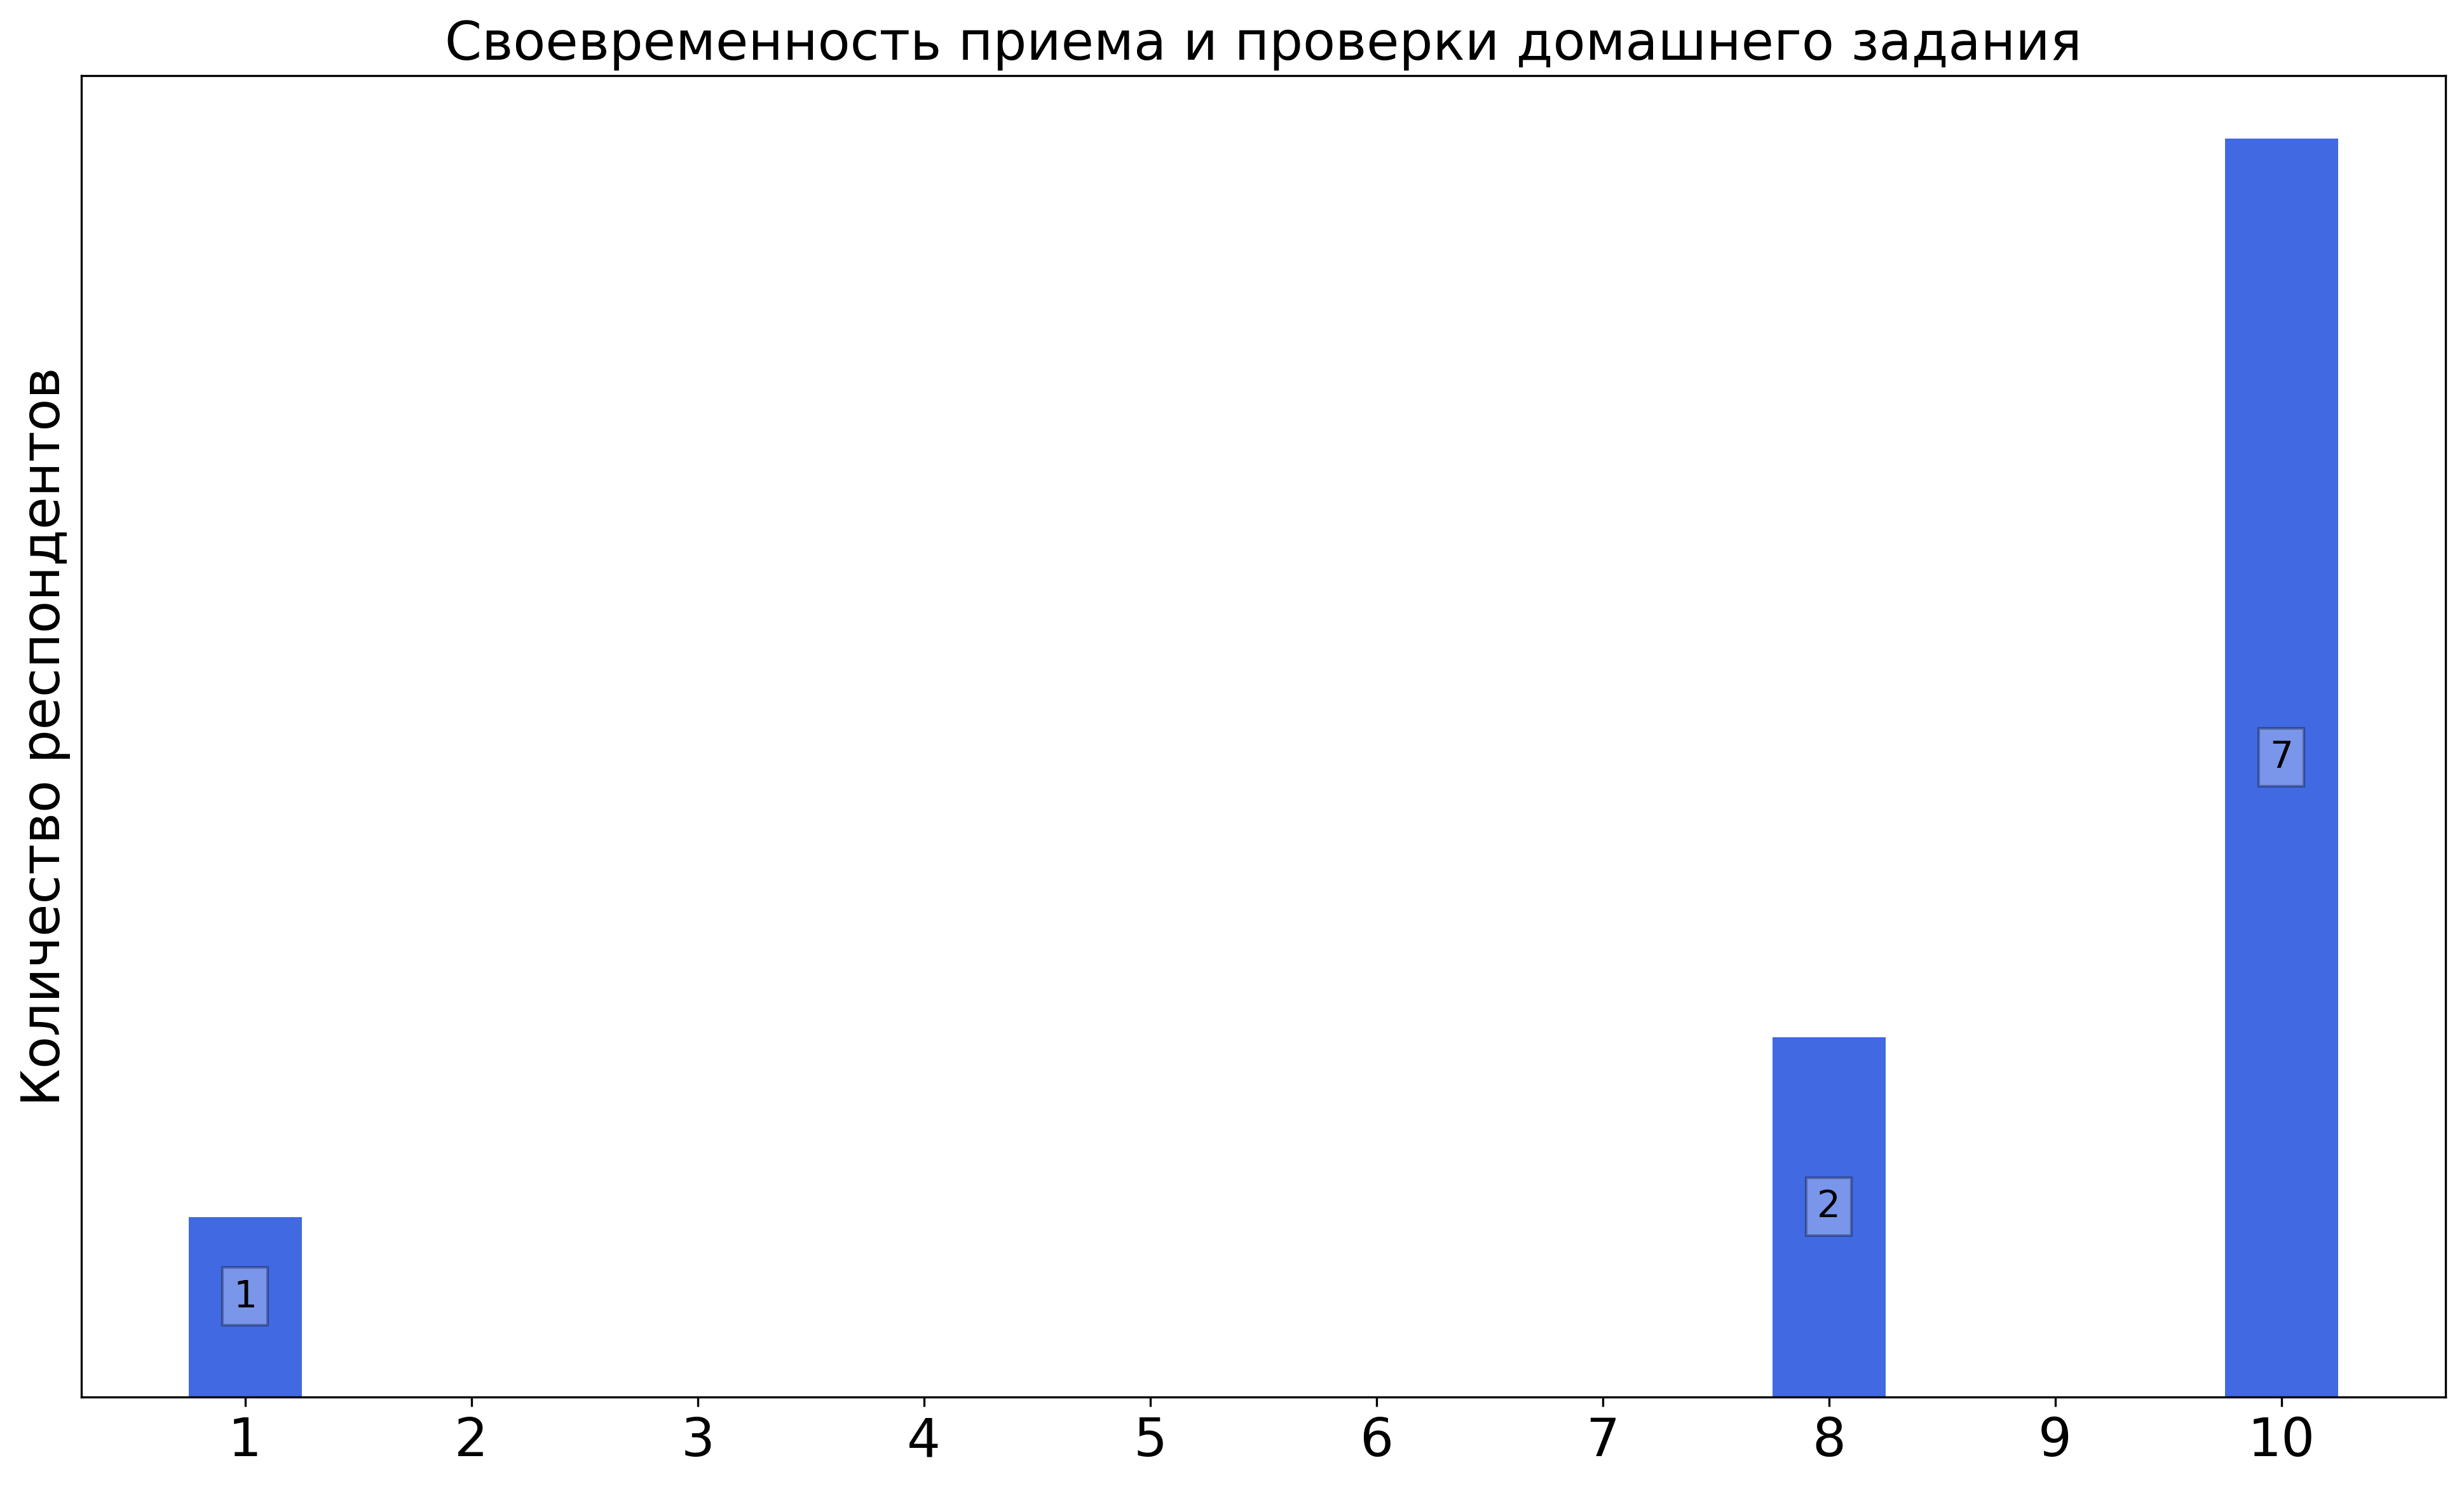
\includegraphics[width=\textwidth]{images/1 course/Информатика/seminarists-marks-Хохлов В.К.-2.png}
			\end{subfigure}
			\begin{subfigure}[b]{0.45\textwidth}
				\centering
				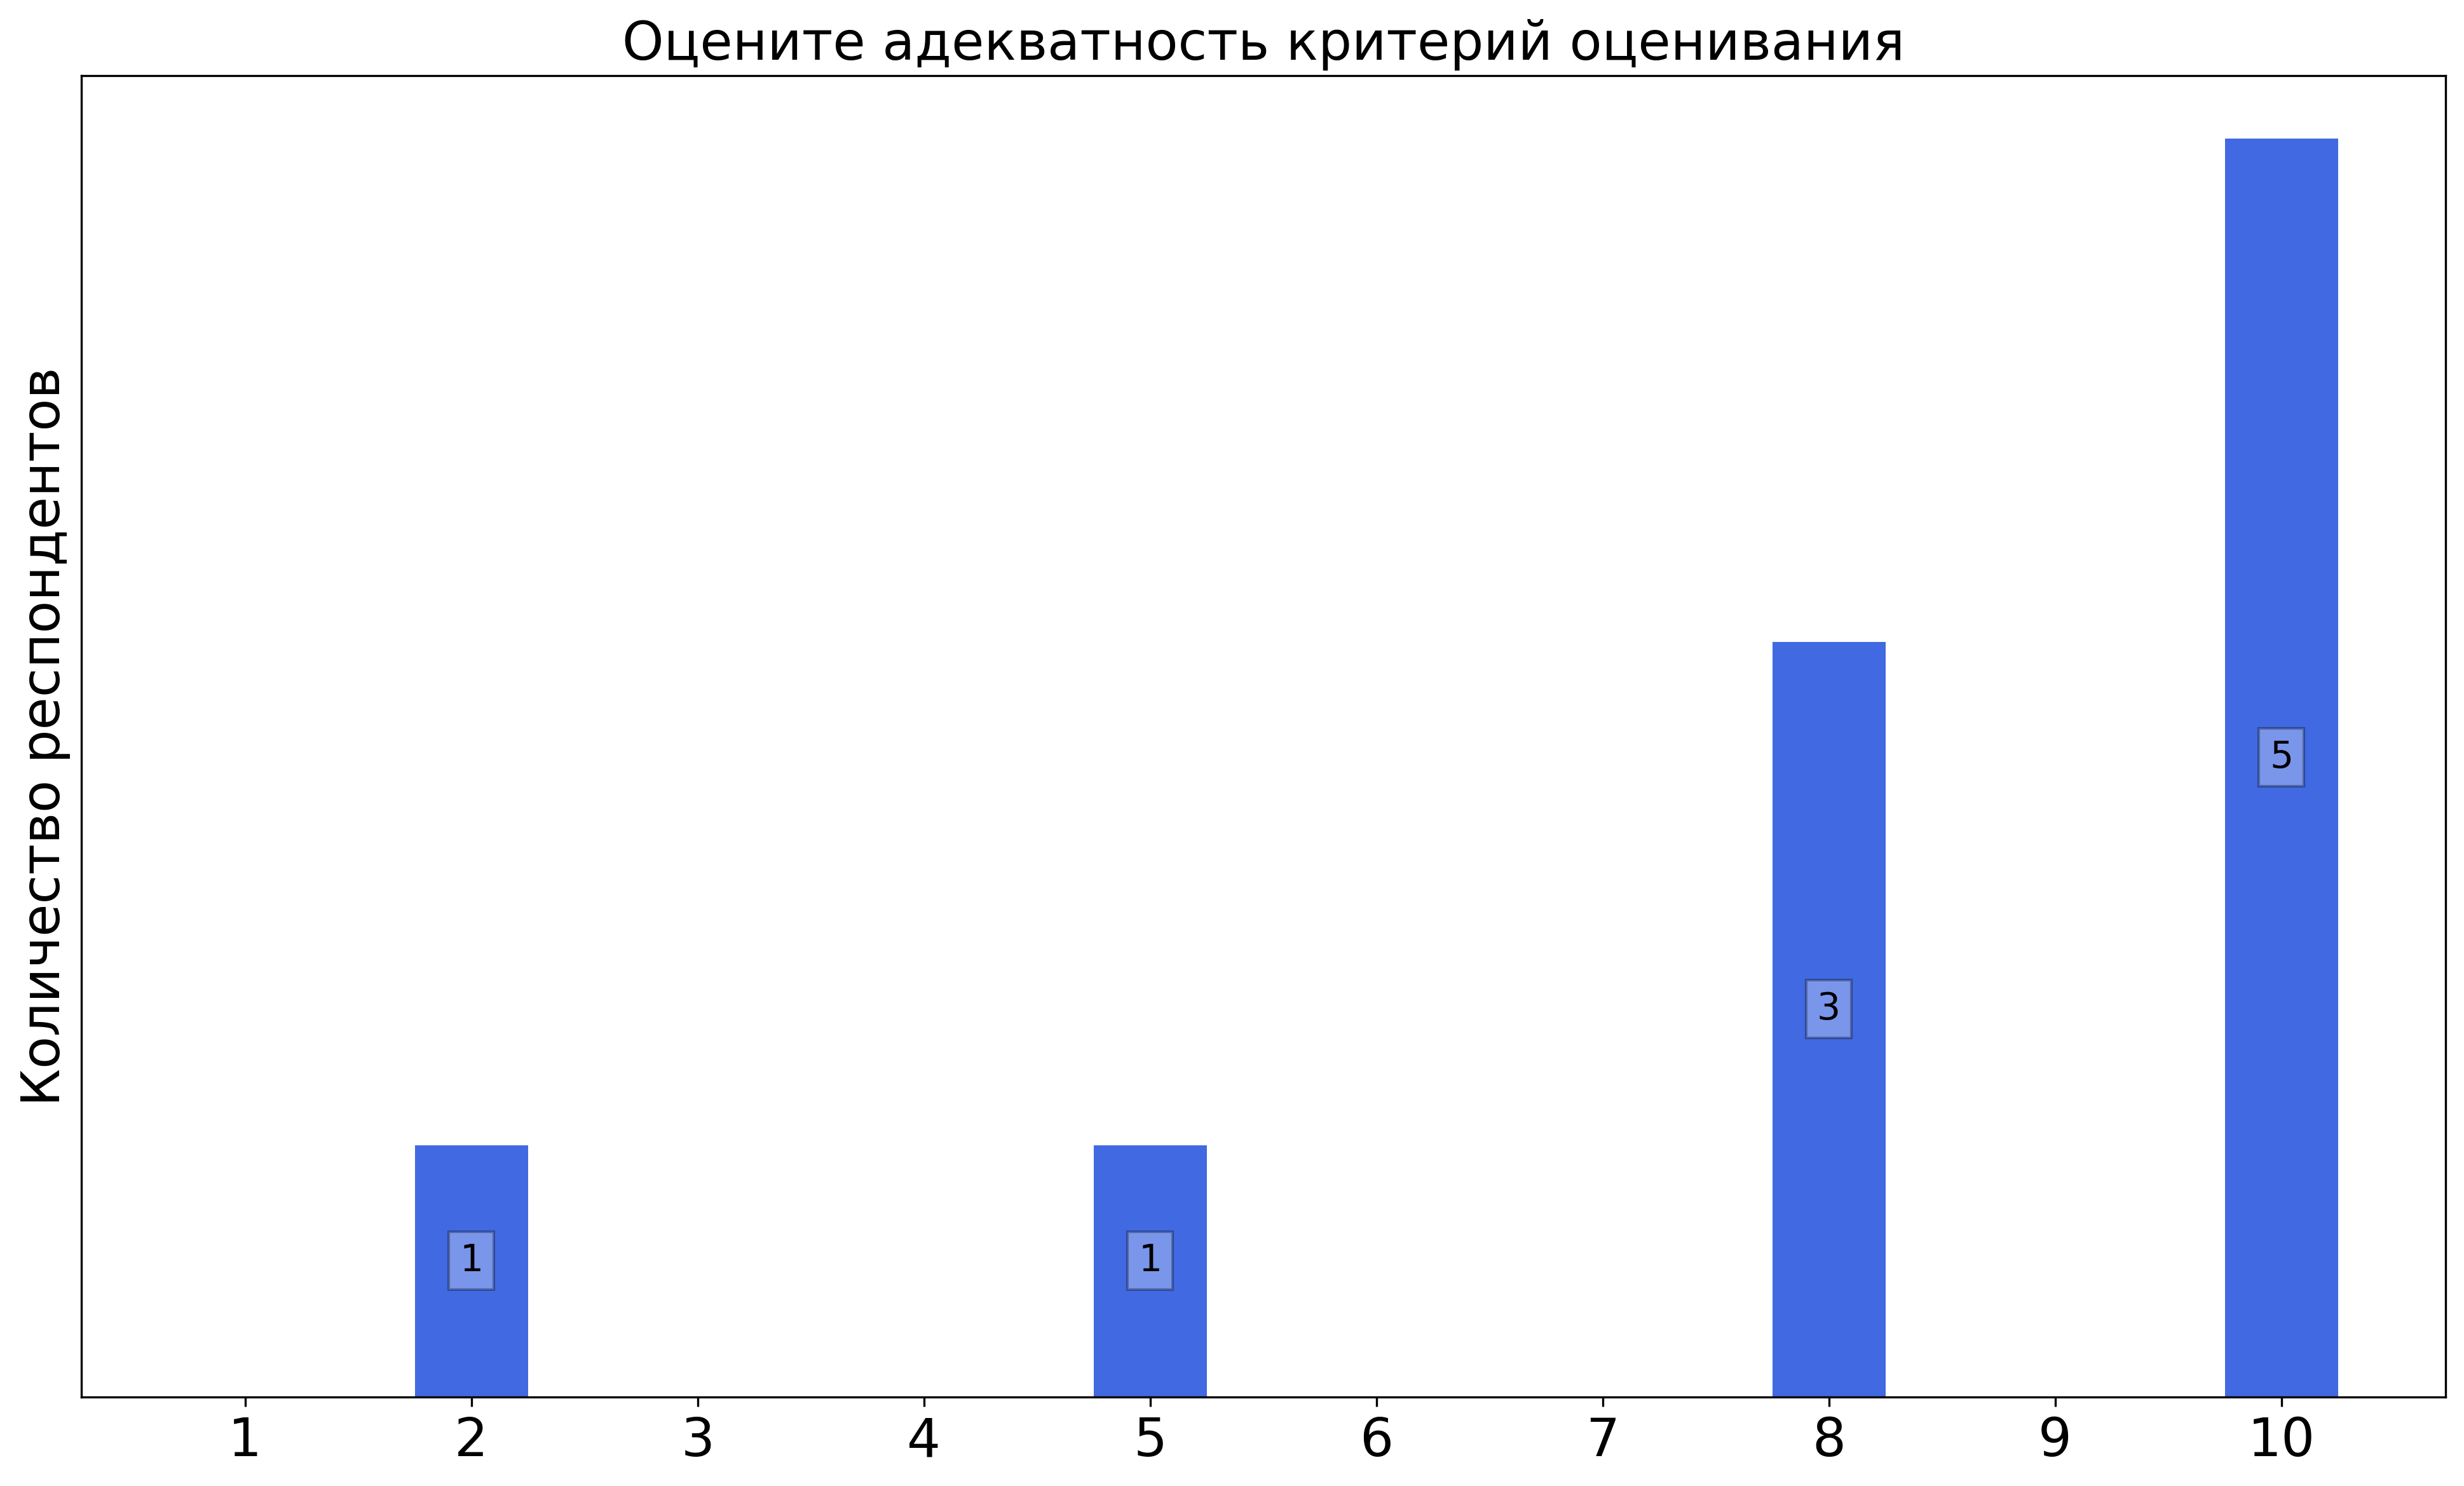
\includegraphics[width=\textwidth]{images/1 course/Информатика/seminarists-marks-Хохлов В.К.-3.png}
			\end{subfigure}	
			\caption{Оценки респондентов о качестве преподавания семинаров}
		\end{figure}

		\textbf{Комментарии студентов о семинаристе\protect\footnote{сохранены оригинальные орфография и пунктуация}}
            \begin{commentbox} 
                Я вообще ничего у него не делал, из его заданий, написал 2 к.р и ушел с 8ой 
            \end{commentbox} 
        
            \begin{commentbox} 
                Почти ничего полезного не получил на семинарах (проходят максимально скучно и нудно, слишком много воды из-за чего просто физически нет возможности что либо пройти), материалы особо не подготавливаются (что есть на компьютере, то и проходим). Единственное хорошее - это максимально снисходительное и человечное отношение к студентам. Очень жаль, что не получил знаний. Хочу к Деду 
            \end{commentbox}

    
    \subsubsection{Отзыв студентов о семинарах. Семинарист: Подлесных Д.А.}
        \begin{figure}[H]
            \centering
            \begin{subfigure}[b]{0.45\textwidth}
                \centering
                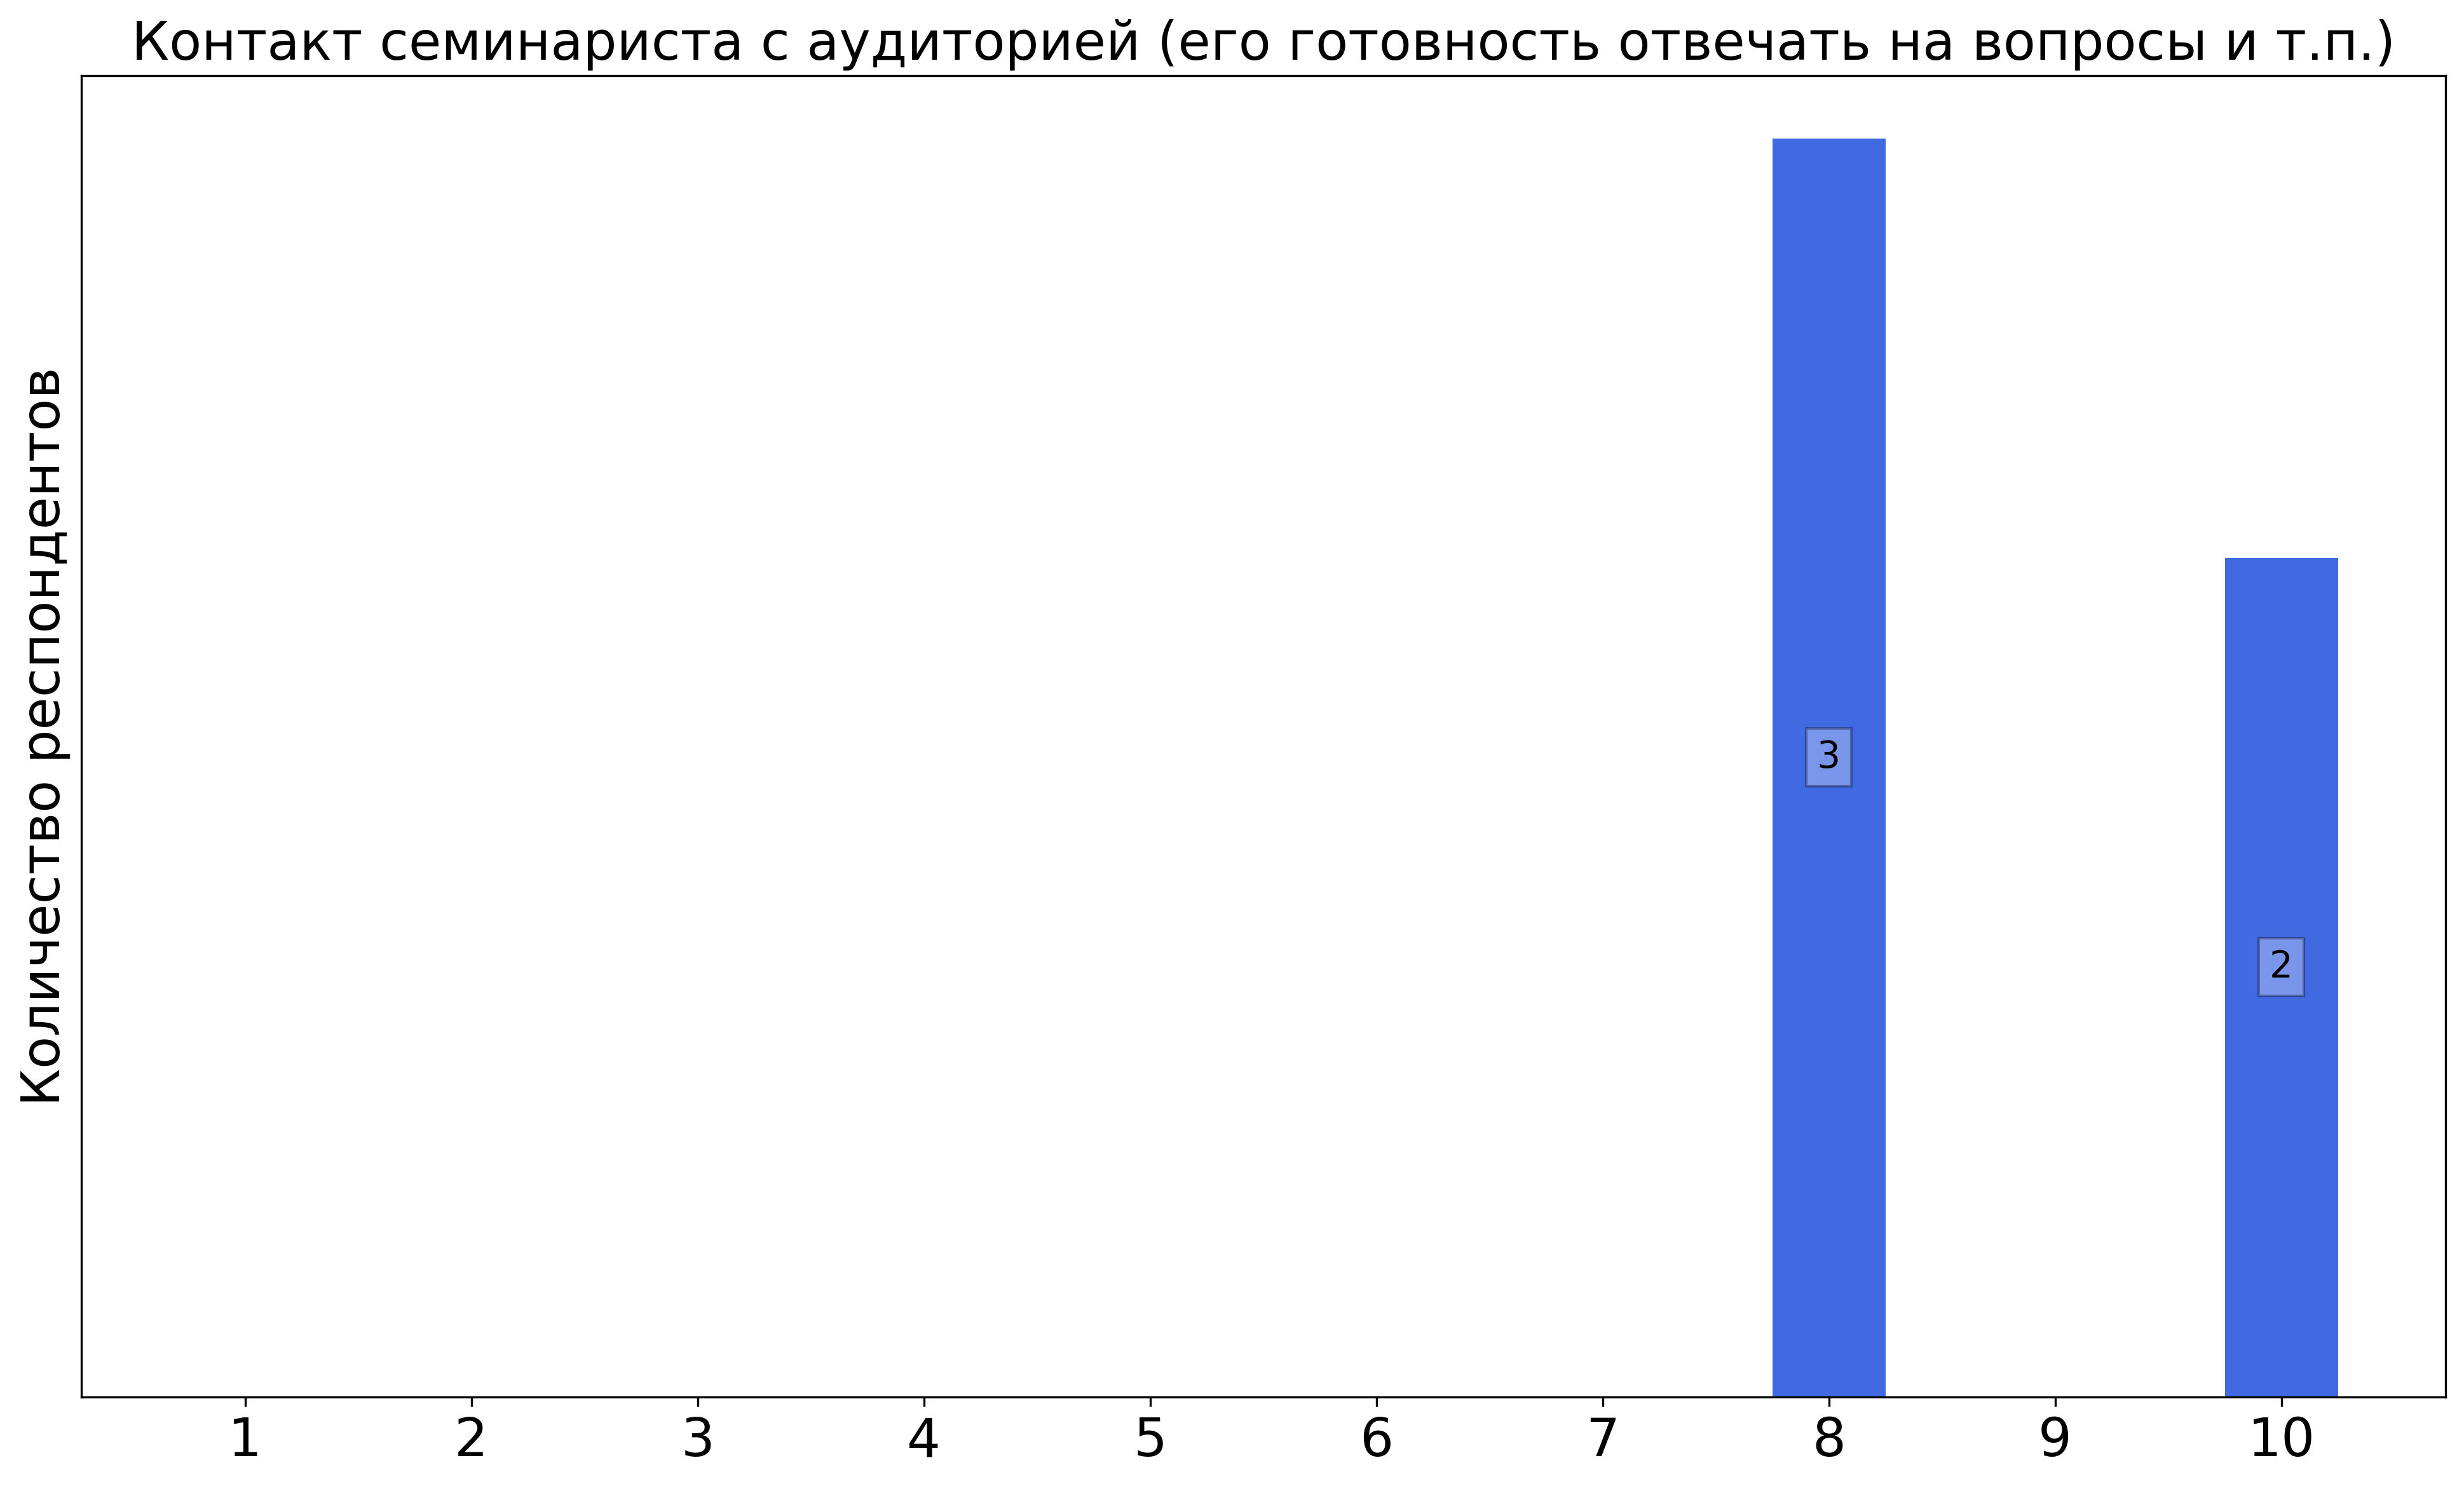
\includegraphics[width=\textwidth]{images/1 course/Информатика/seminarists-marks-Подлесных Д.А.-0.png}
            \end{subfigure}
            \begin{subfigure}[b]{0.45\textwidth}
                \centering
                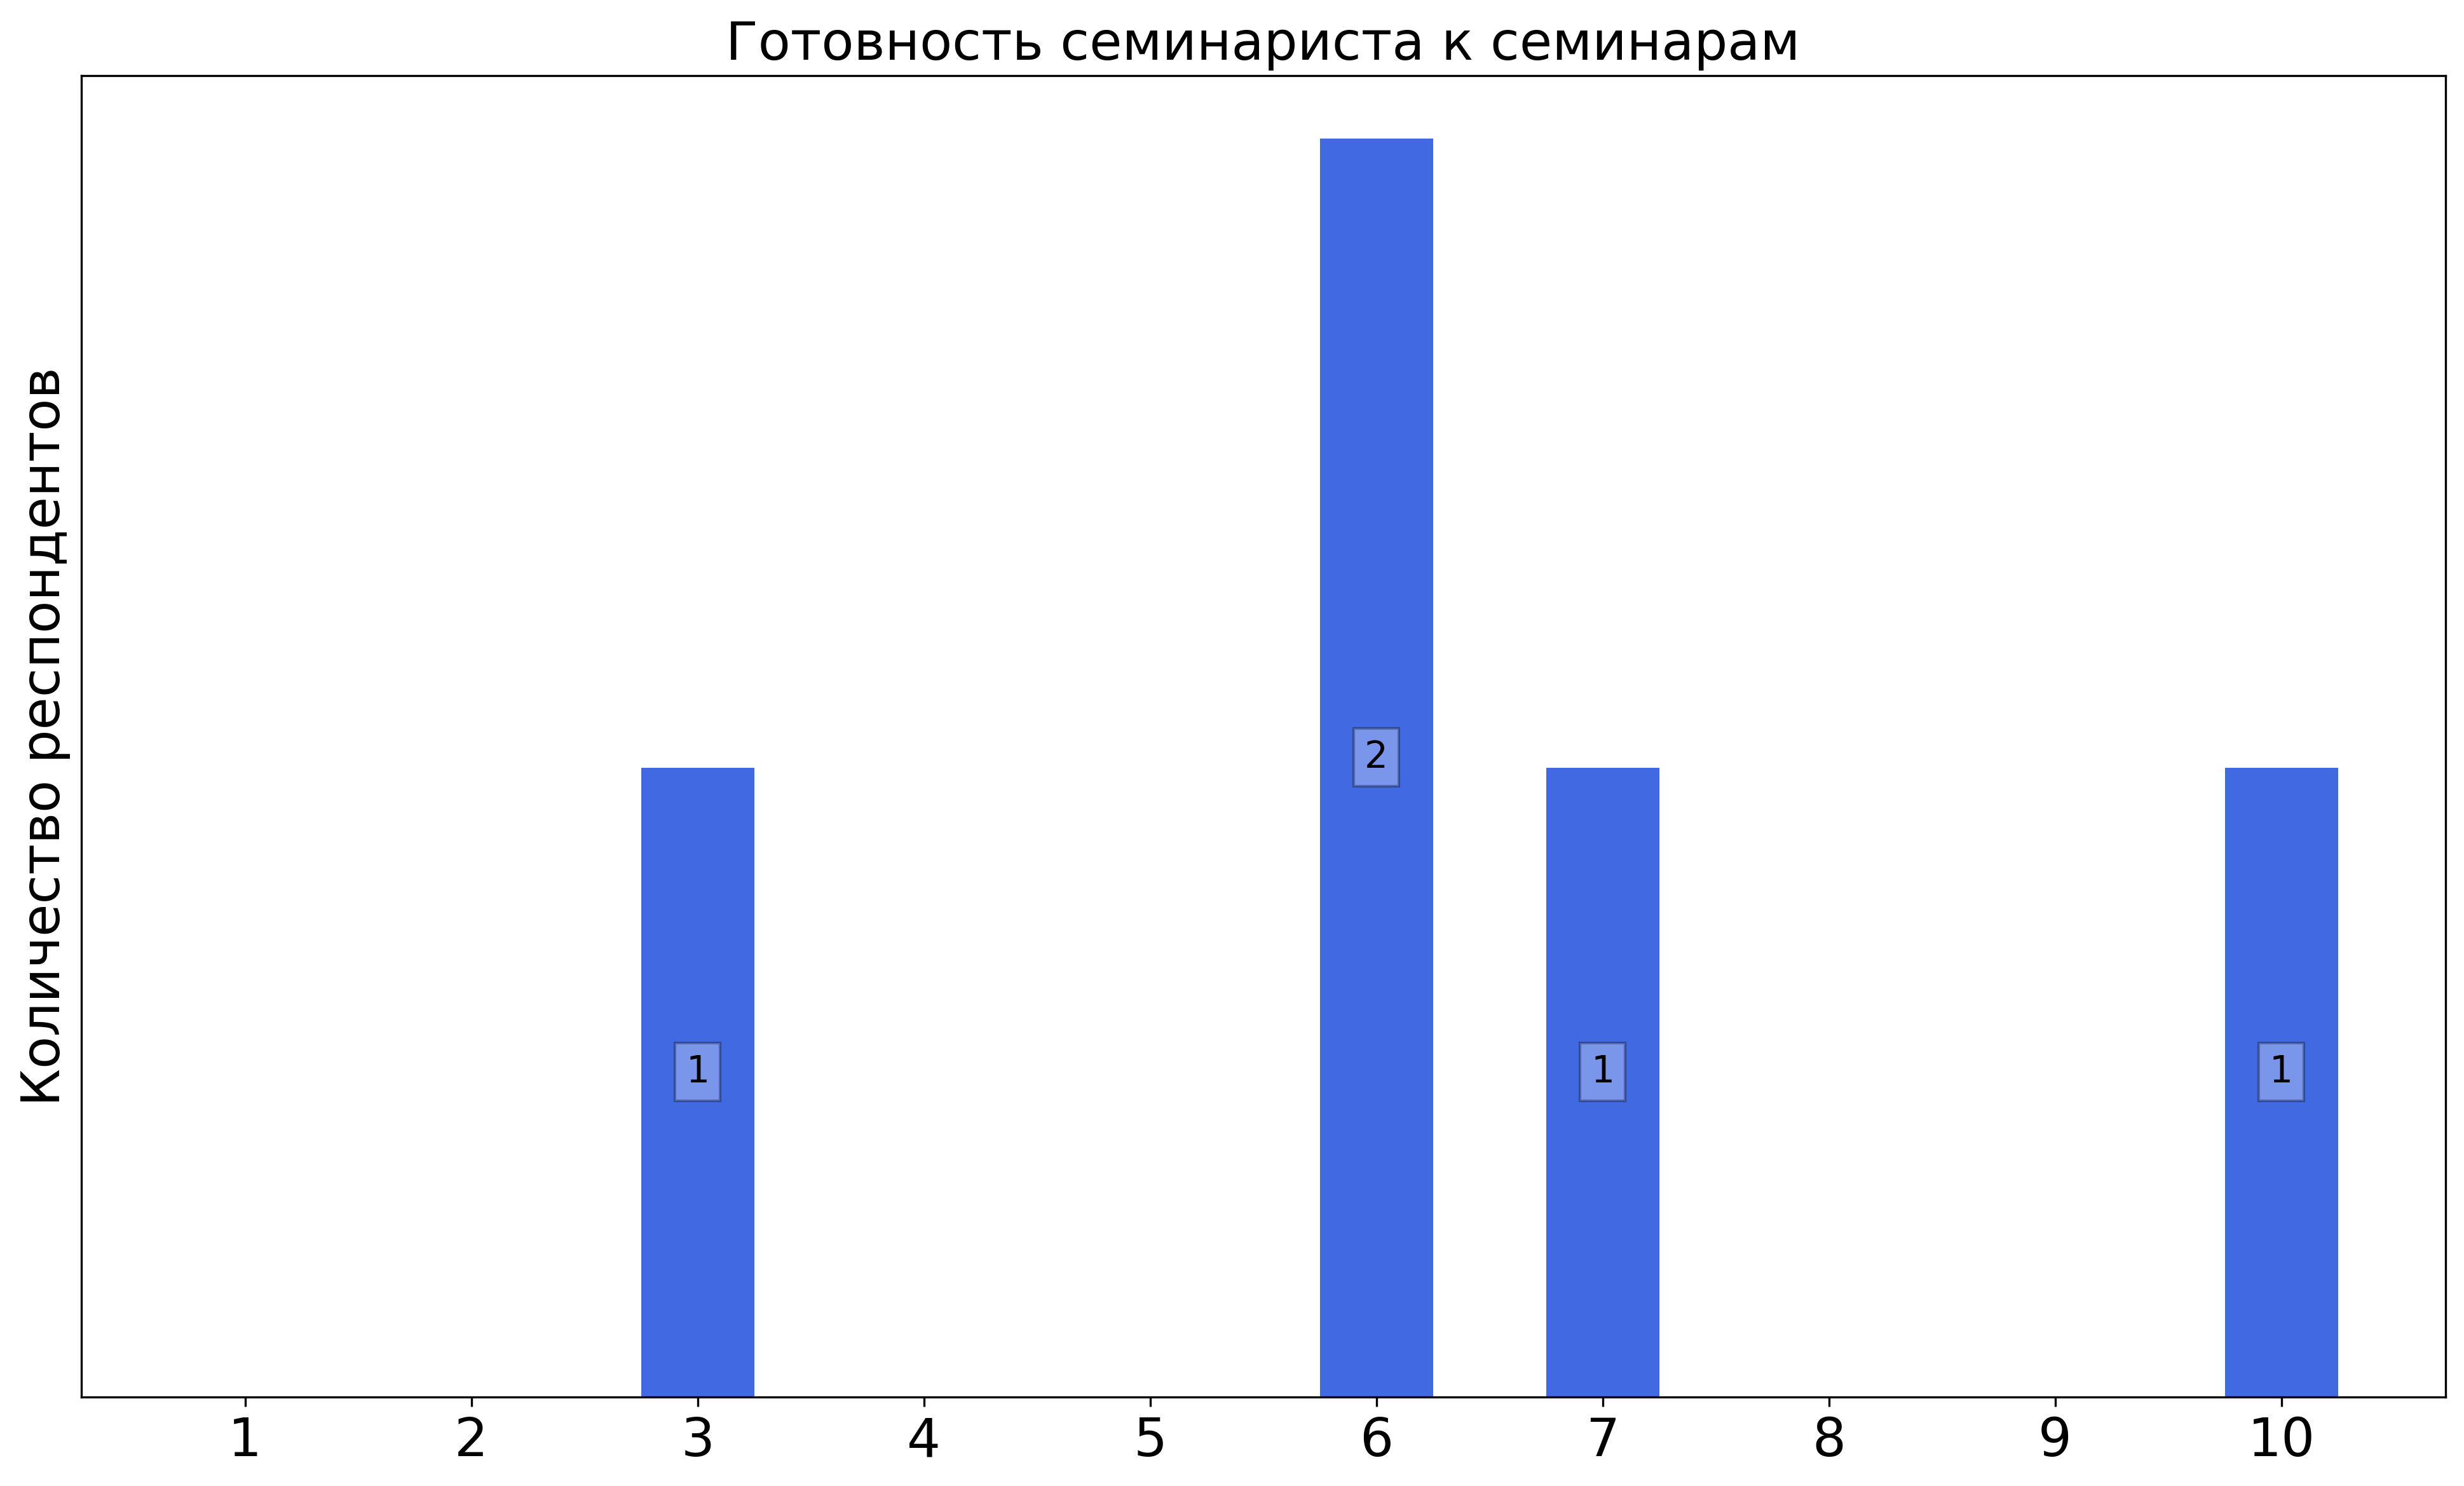
\includegraphics[width=\textwidth]{images/1 course/Информатика/seminarists-marks-Подлесных Д.А.-1.png}
            \end{subfigure}
            \begin{subfigure}[b]{0.45\textwidth}
                \centering
                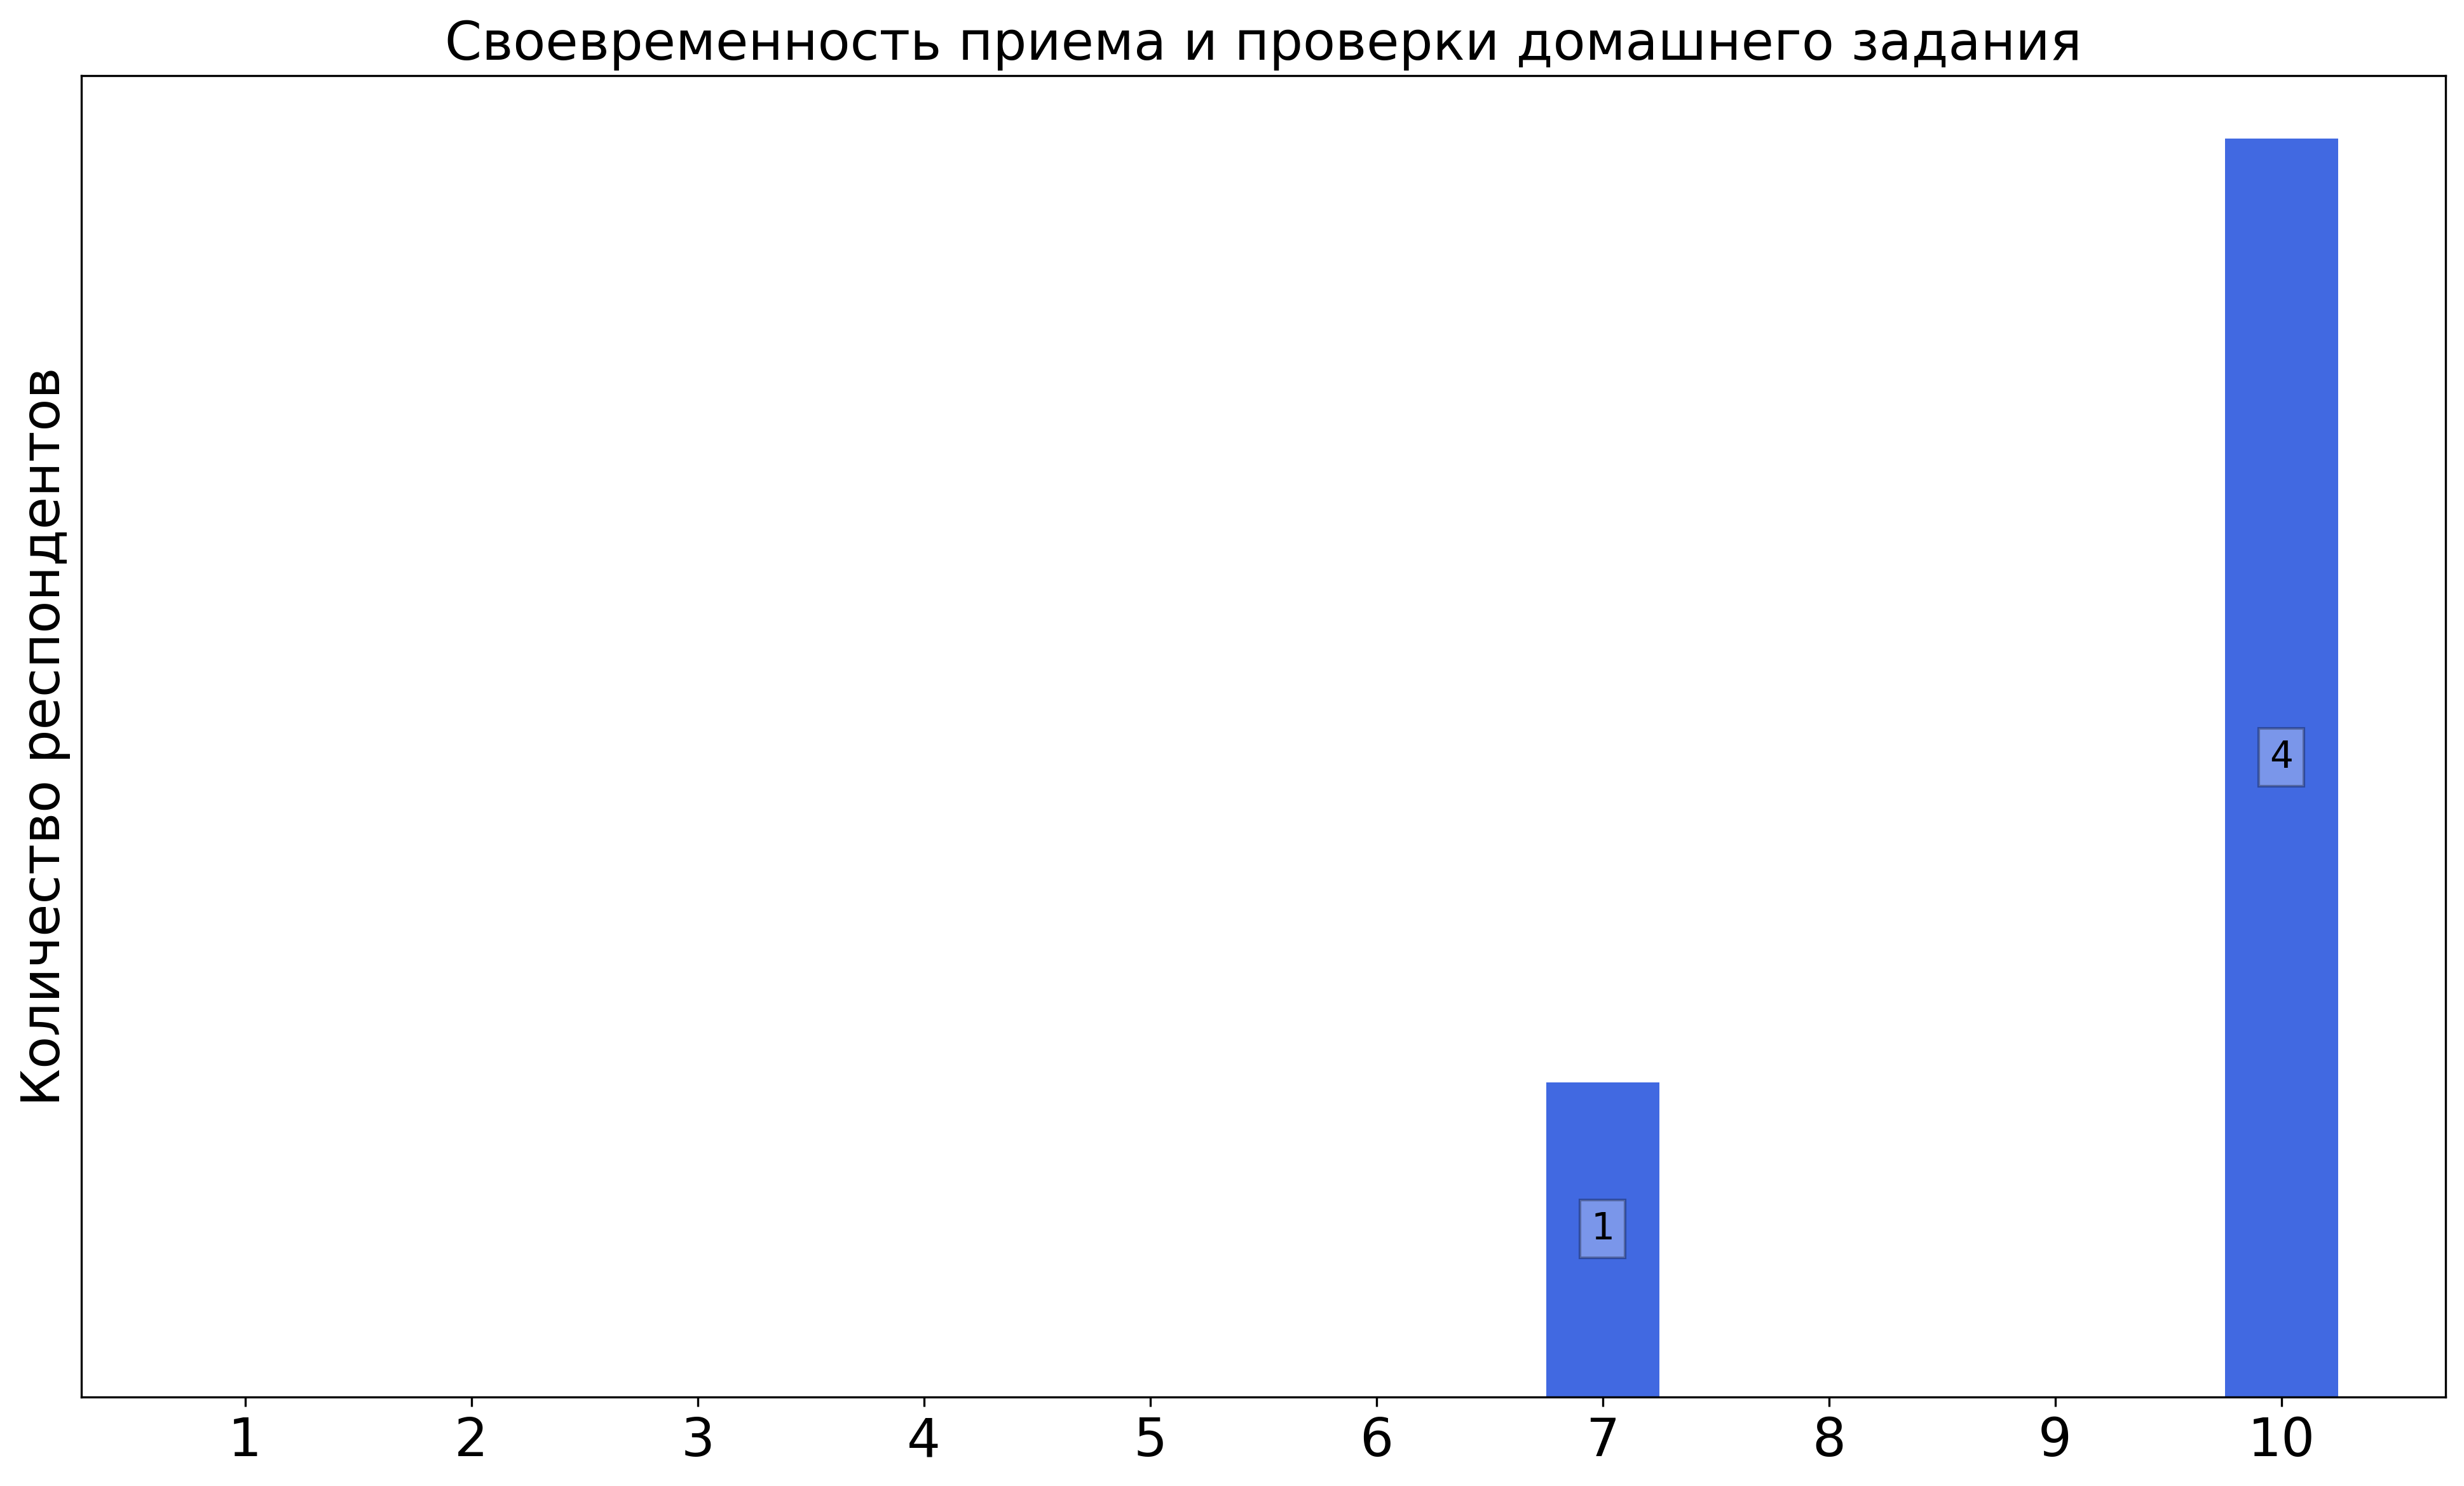
\includegraphics[width=\textwidth]{images/1 course/Информатика/seminarists-marks-Подлесных Д.А.-2.png}
            \end{subfigure}
            \begin{subfigure}[b]{0.45\textwidth}
                \centering
                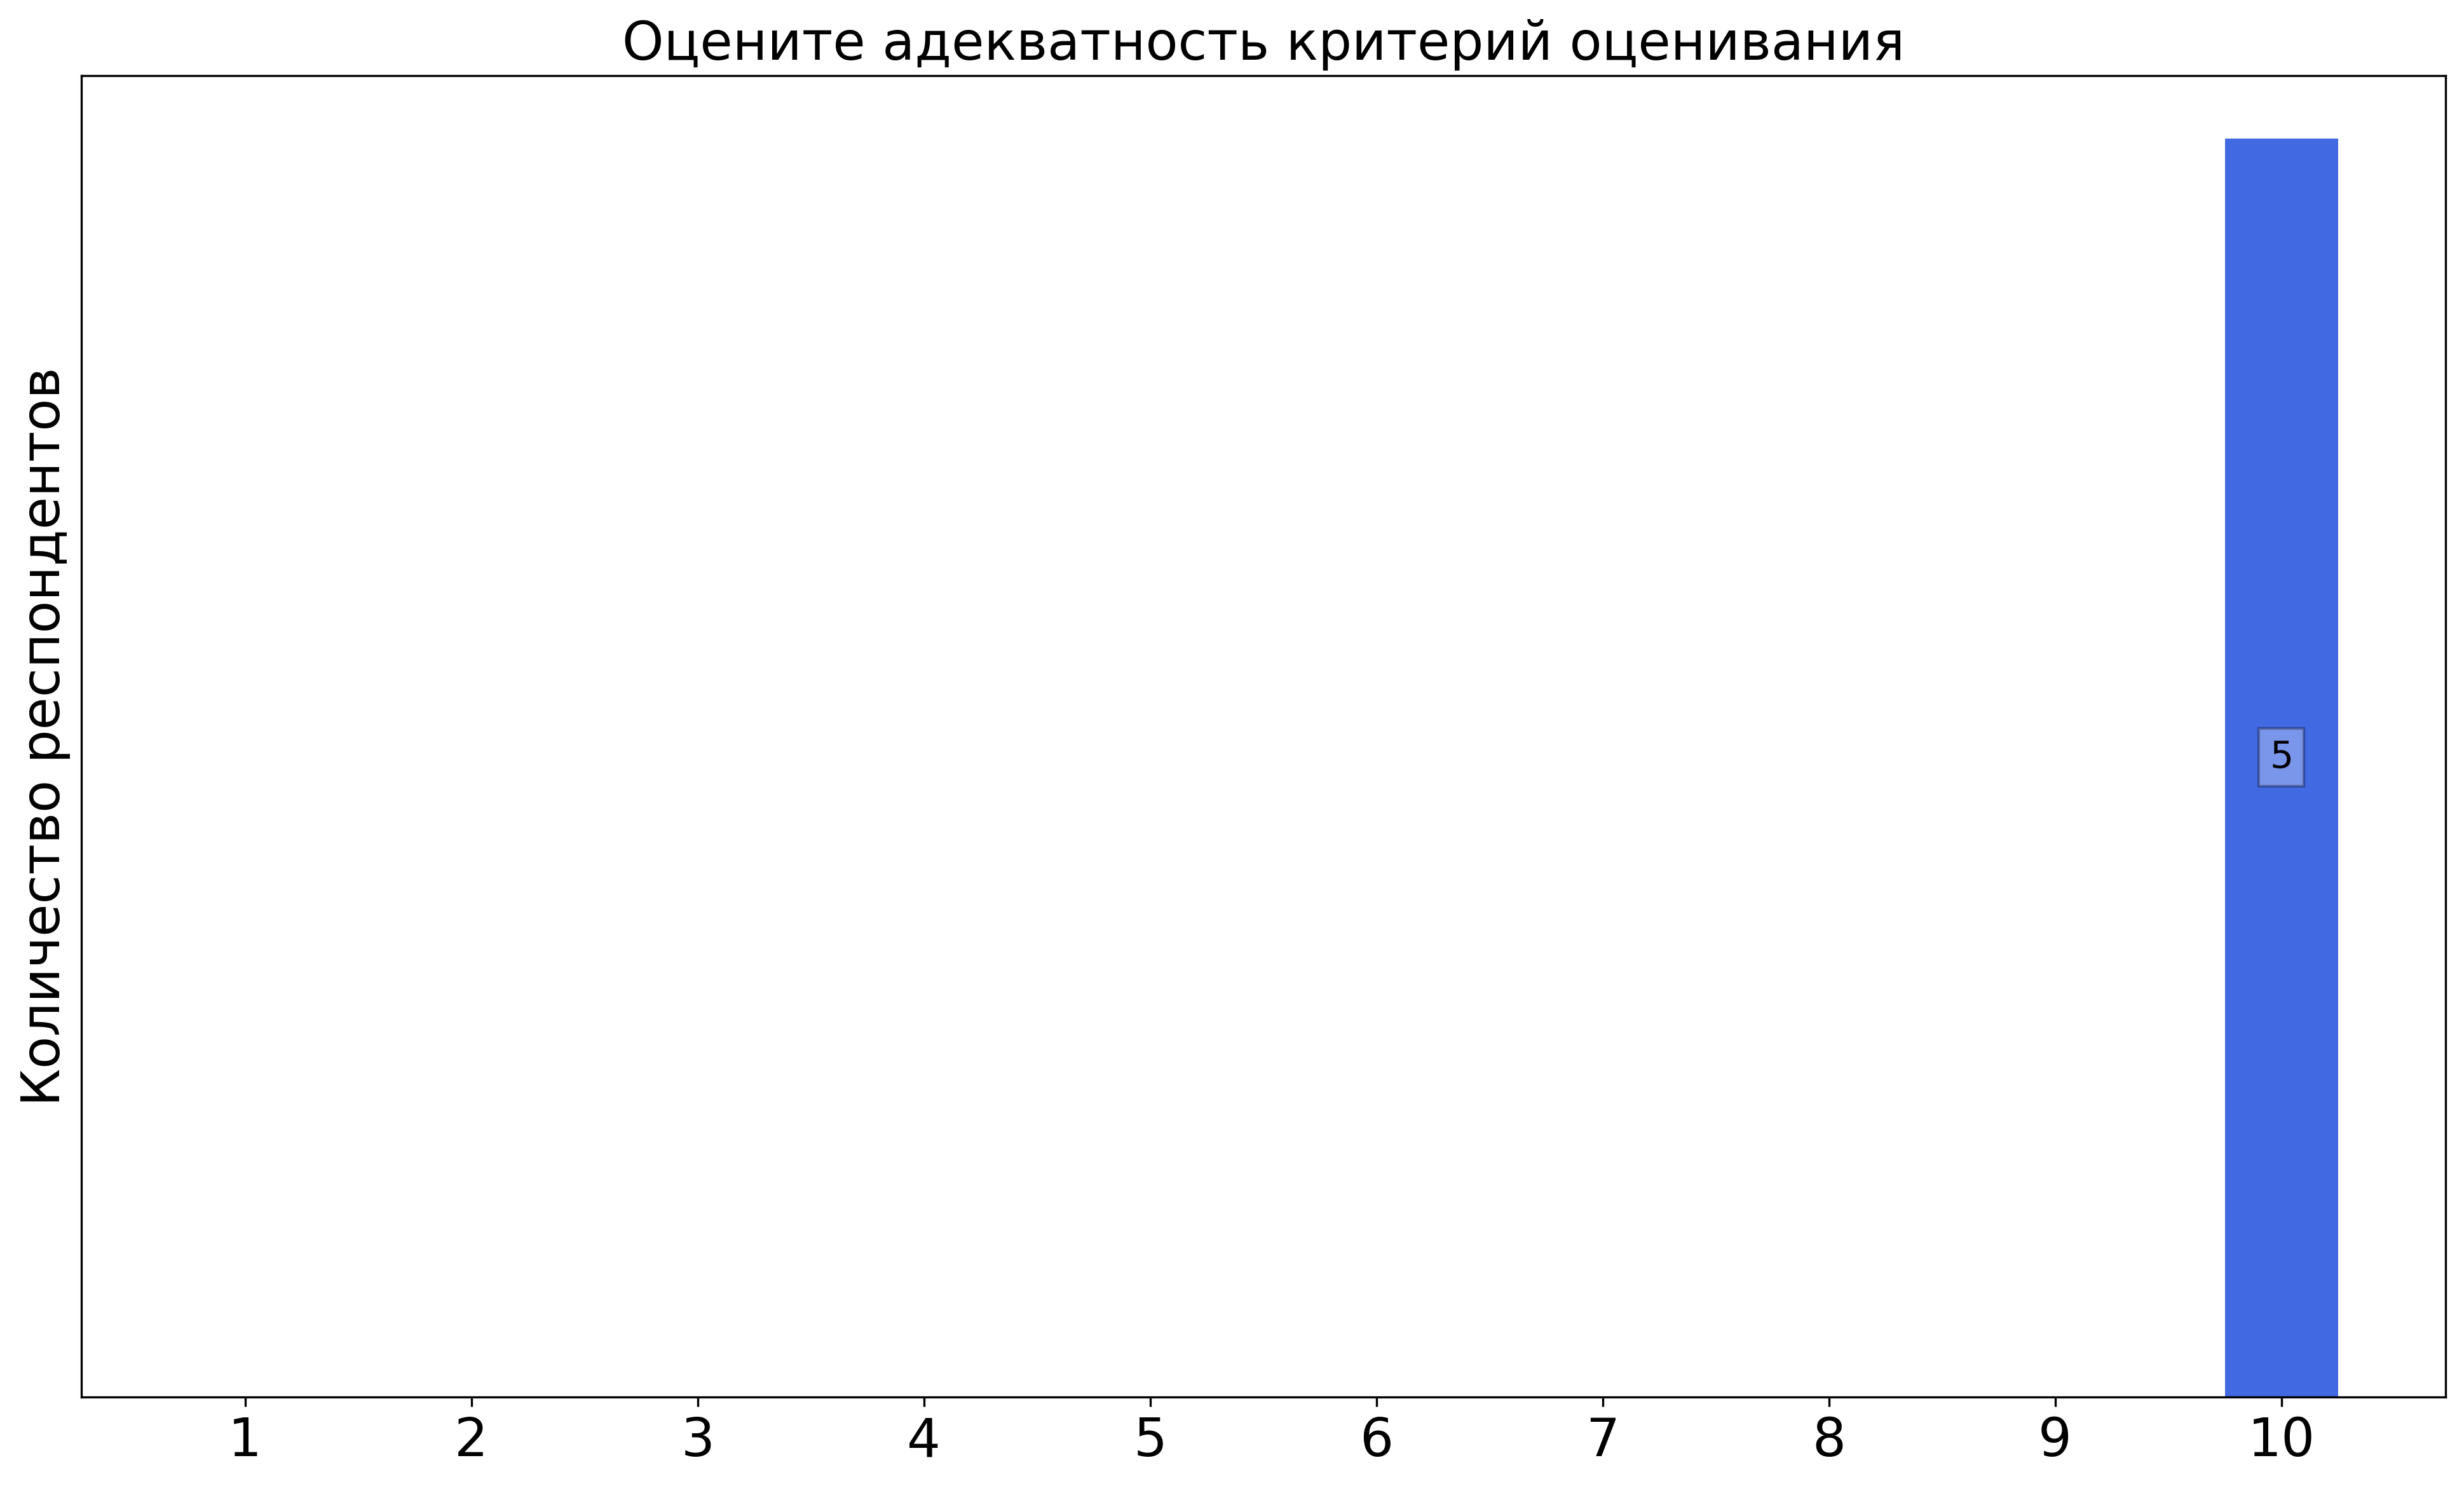
\includegraphics[width=\textwidth]{images/1 course/Информатика/seminarists-marks-Подлесных Д.А.-3.png}
            \end{subfigure}	
            \caption{Оценки респондентов о качестве преподавания семинаров}
        \end{figure}

        \textbf{Комментарии студентов о семинаристе\protect\footnote{сохранены оригинальные орфография и пунктуация}}
            \begin{commentbox} 
                Немного странный подход. Иногда тупо решали контест, это как бы норм, но на фоне еще разбирались задачи с него. Но никто не слушает, потому что все решают с разным темпом, поэтому польза от этого невелика. А так шарящий семер за прогу 
            \end{commentbox}

        
    \subsubsection{Отзыв студентов о семинарах. Семинарист: Кулиев Р.С.}
        \begin{figure}[H]
            \centering
            \begin{subfigure}[b]{0.45\textwidth}
                \centering
                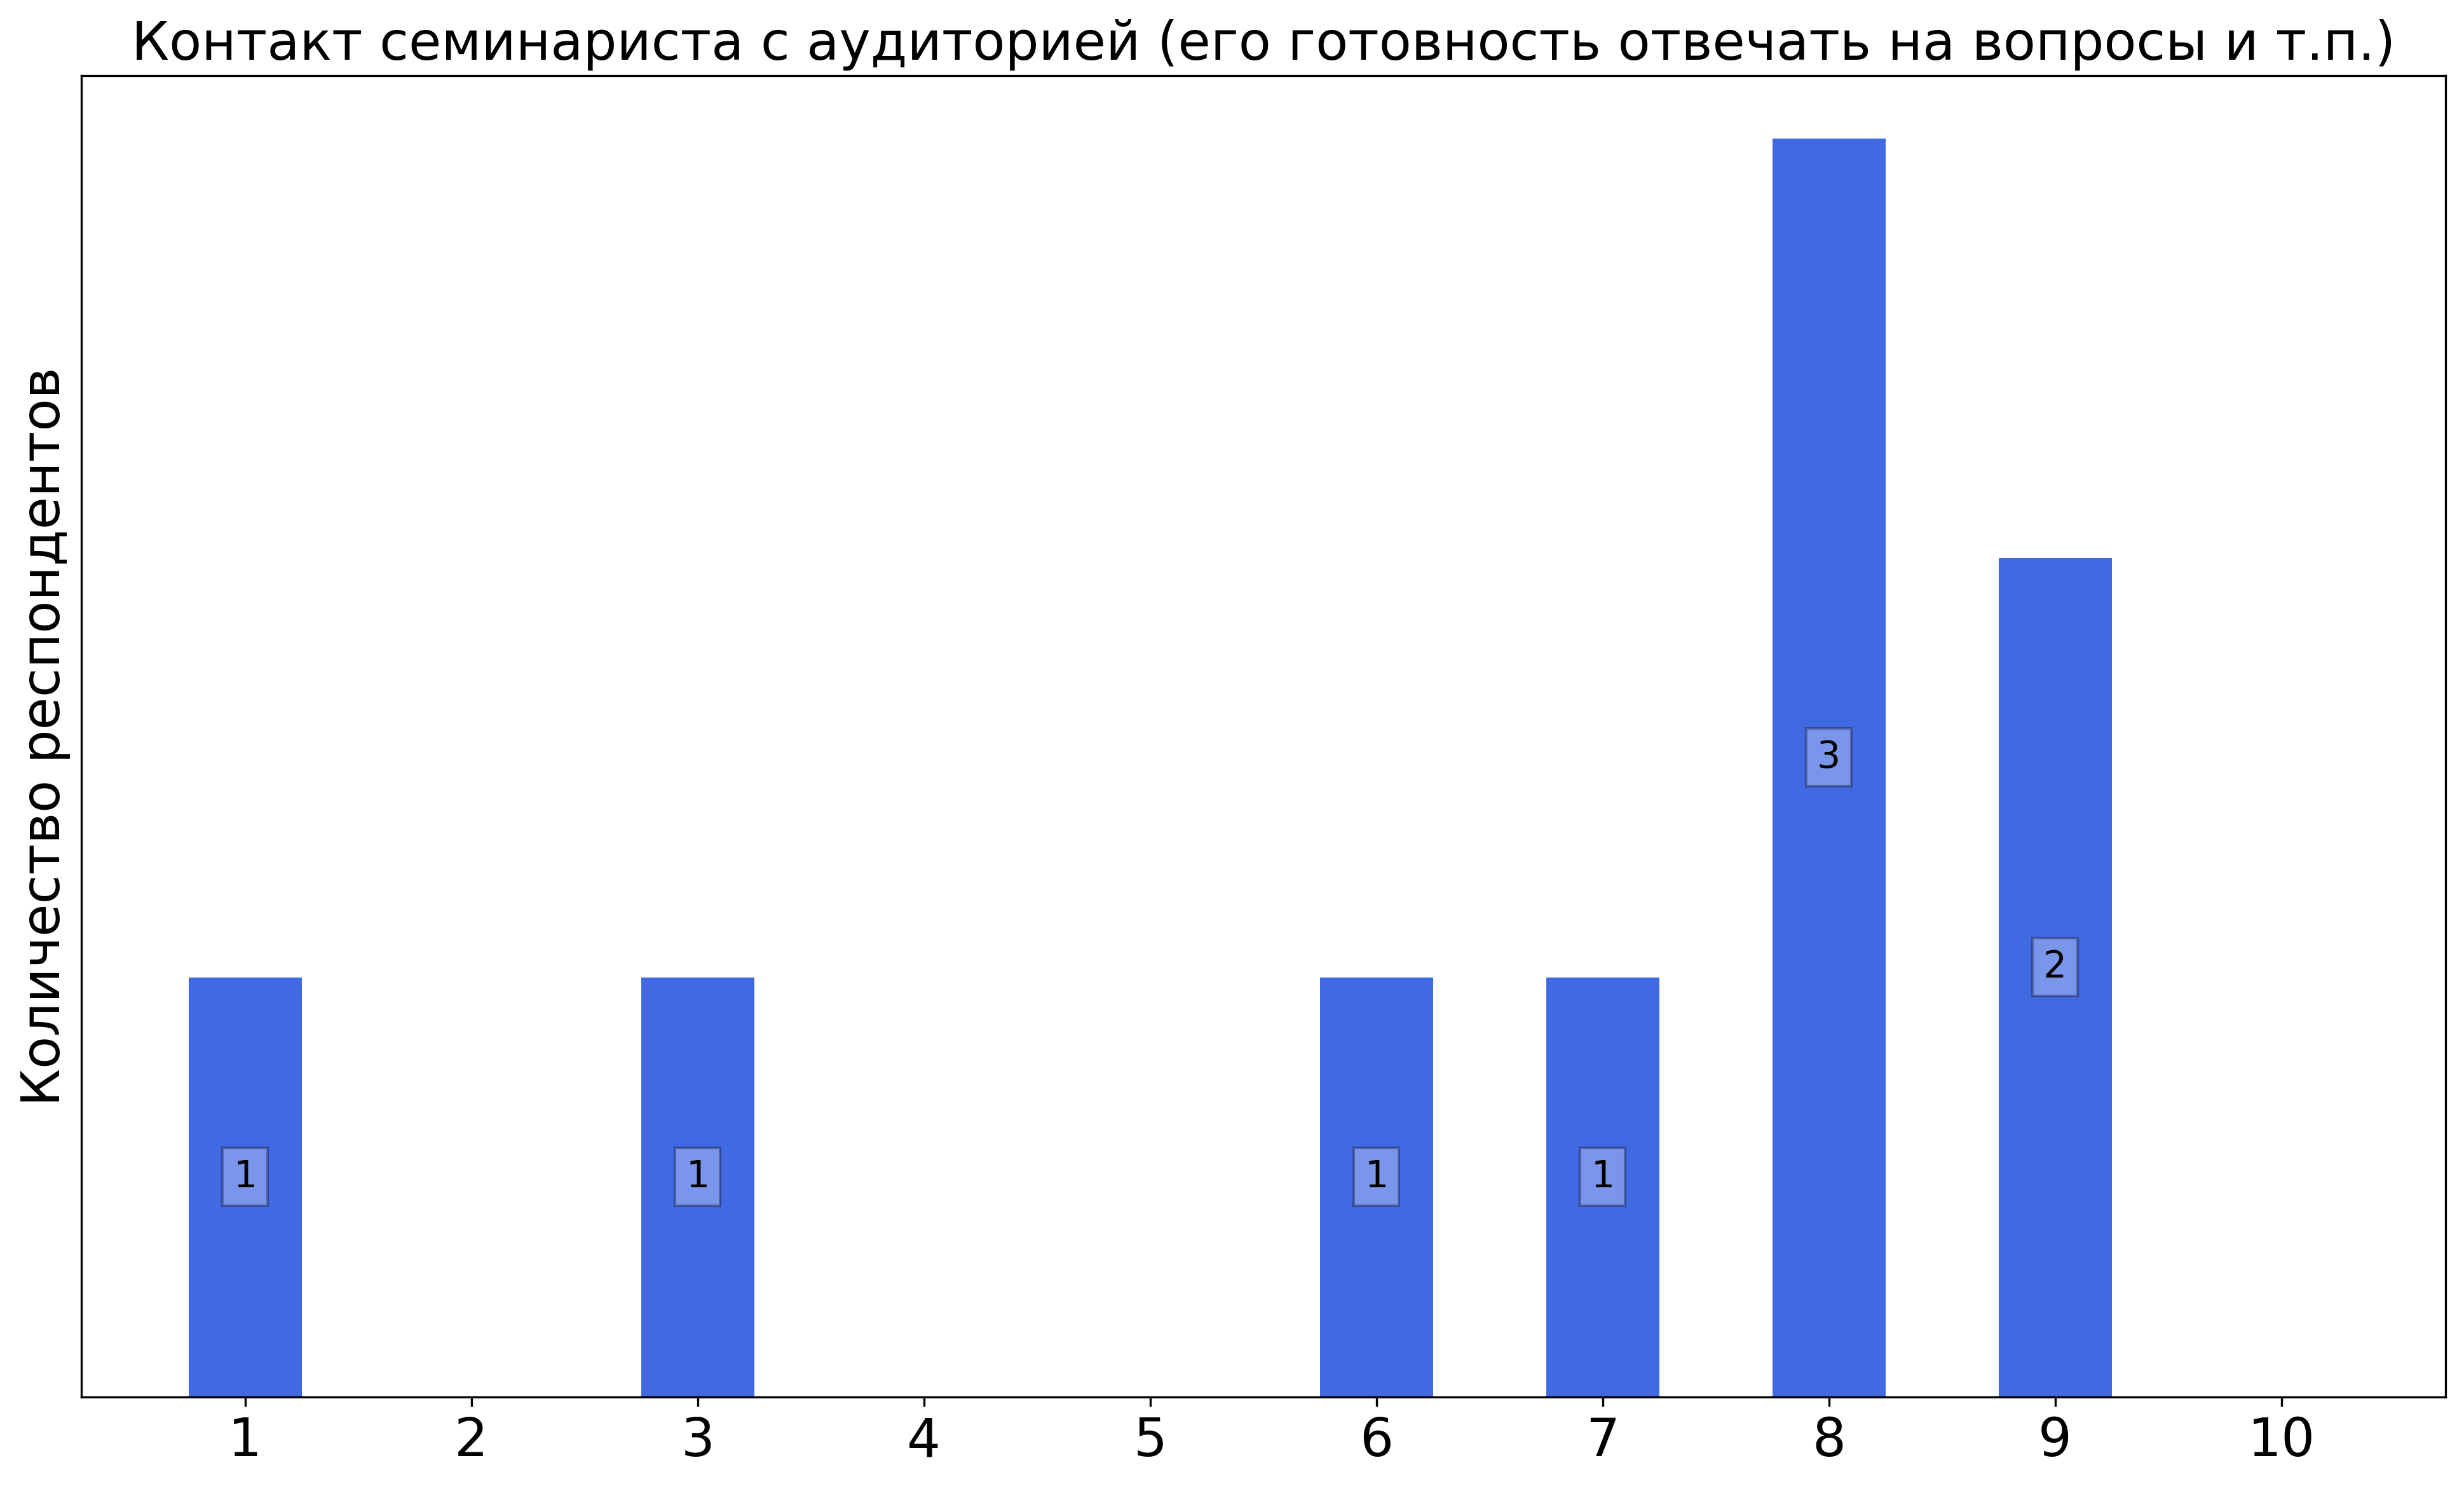
\includegraphics[width=\textwidth]{images/1 course/Информатика/seminarists-marks-Кулиев Р.С.-0.png}
            \end{subfigure}
            \begin{subfigure}[b]{0.45\textwidth}
                \centering
                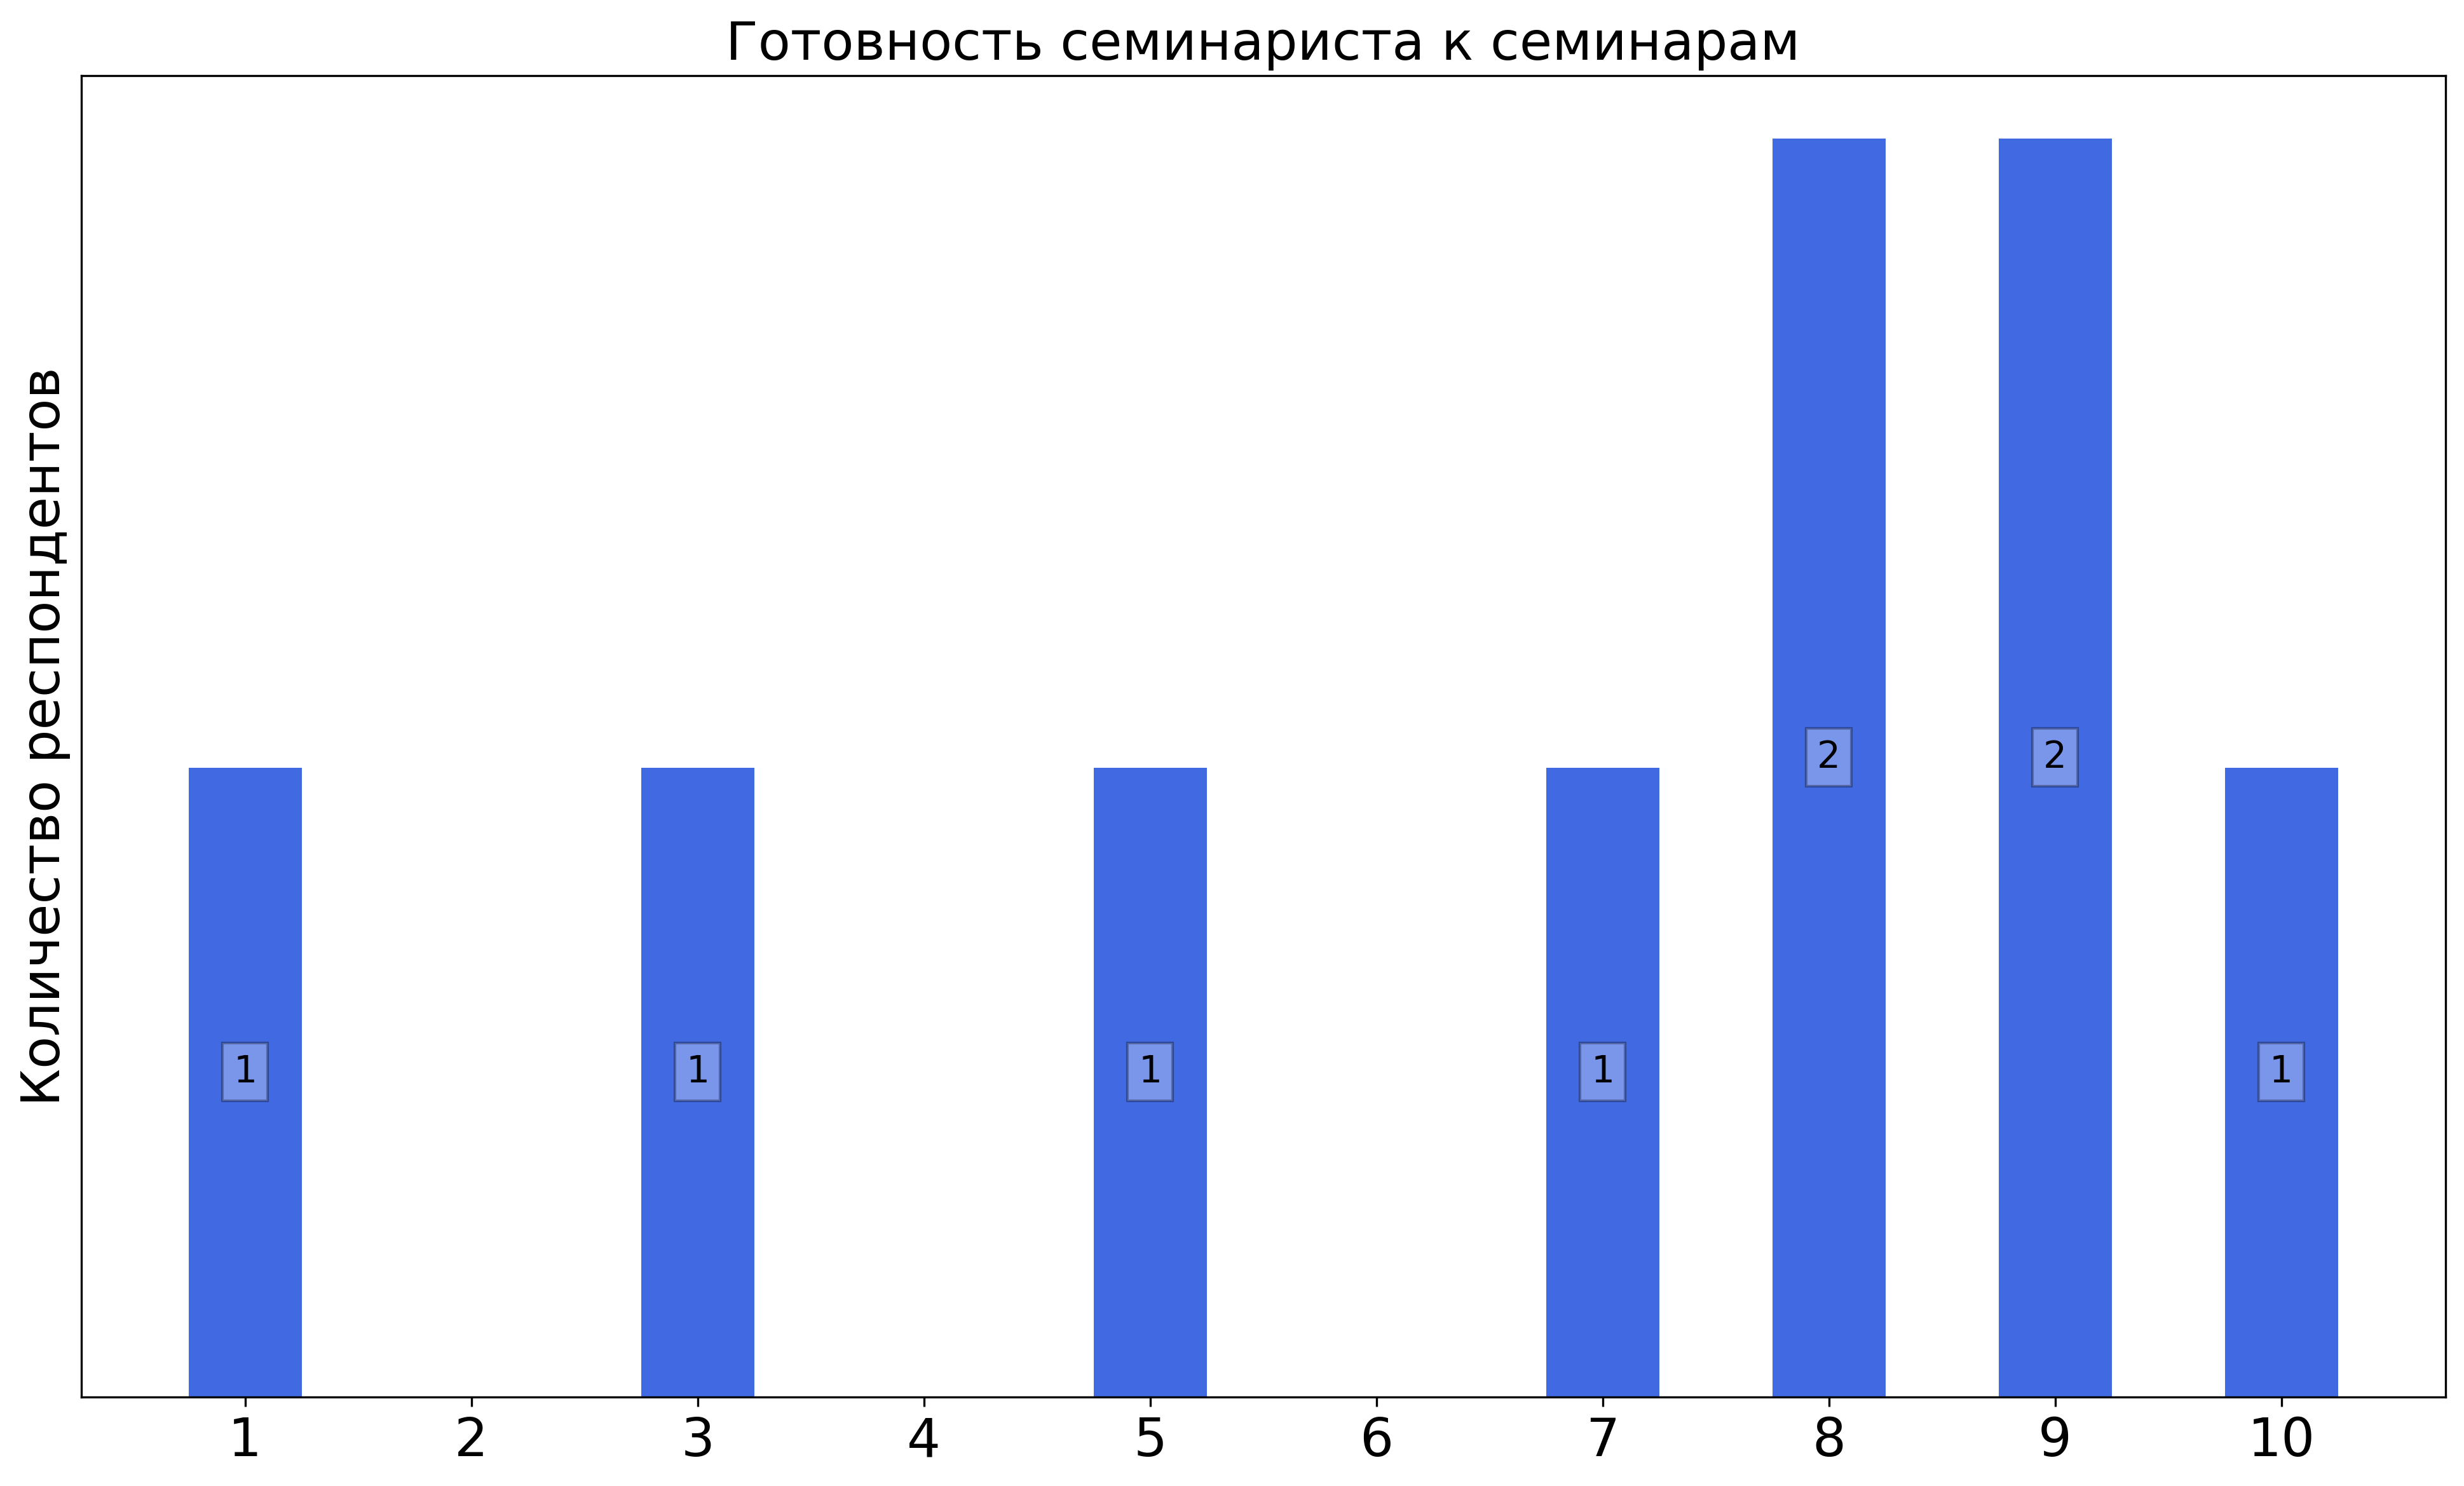
\includegraphics[width=\textwidth]{images/1 course/Информатика/seminarists-marks-Кулиев Р.С.-1.png}
            \end{subfigure}
            \begin{subfigure}[b]{0.45\textwidth}
                \centering
                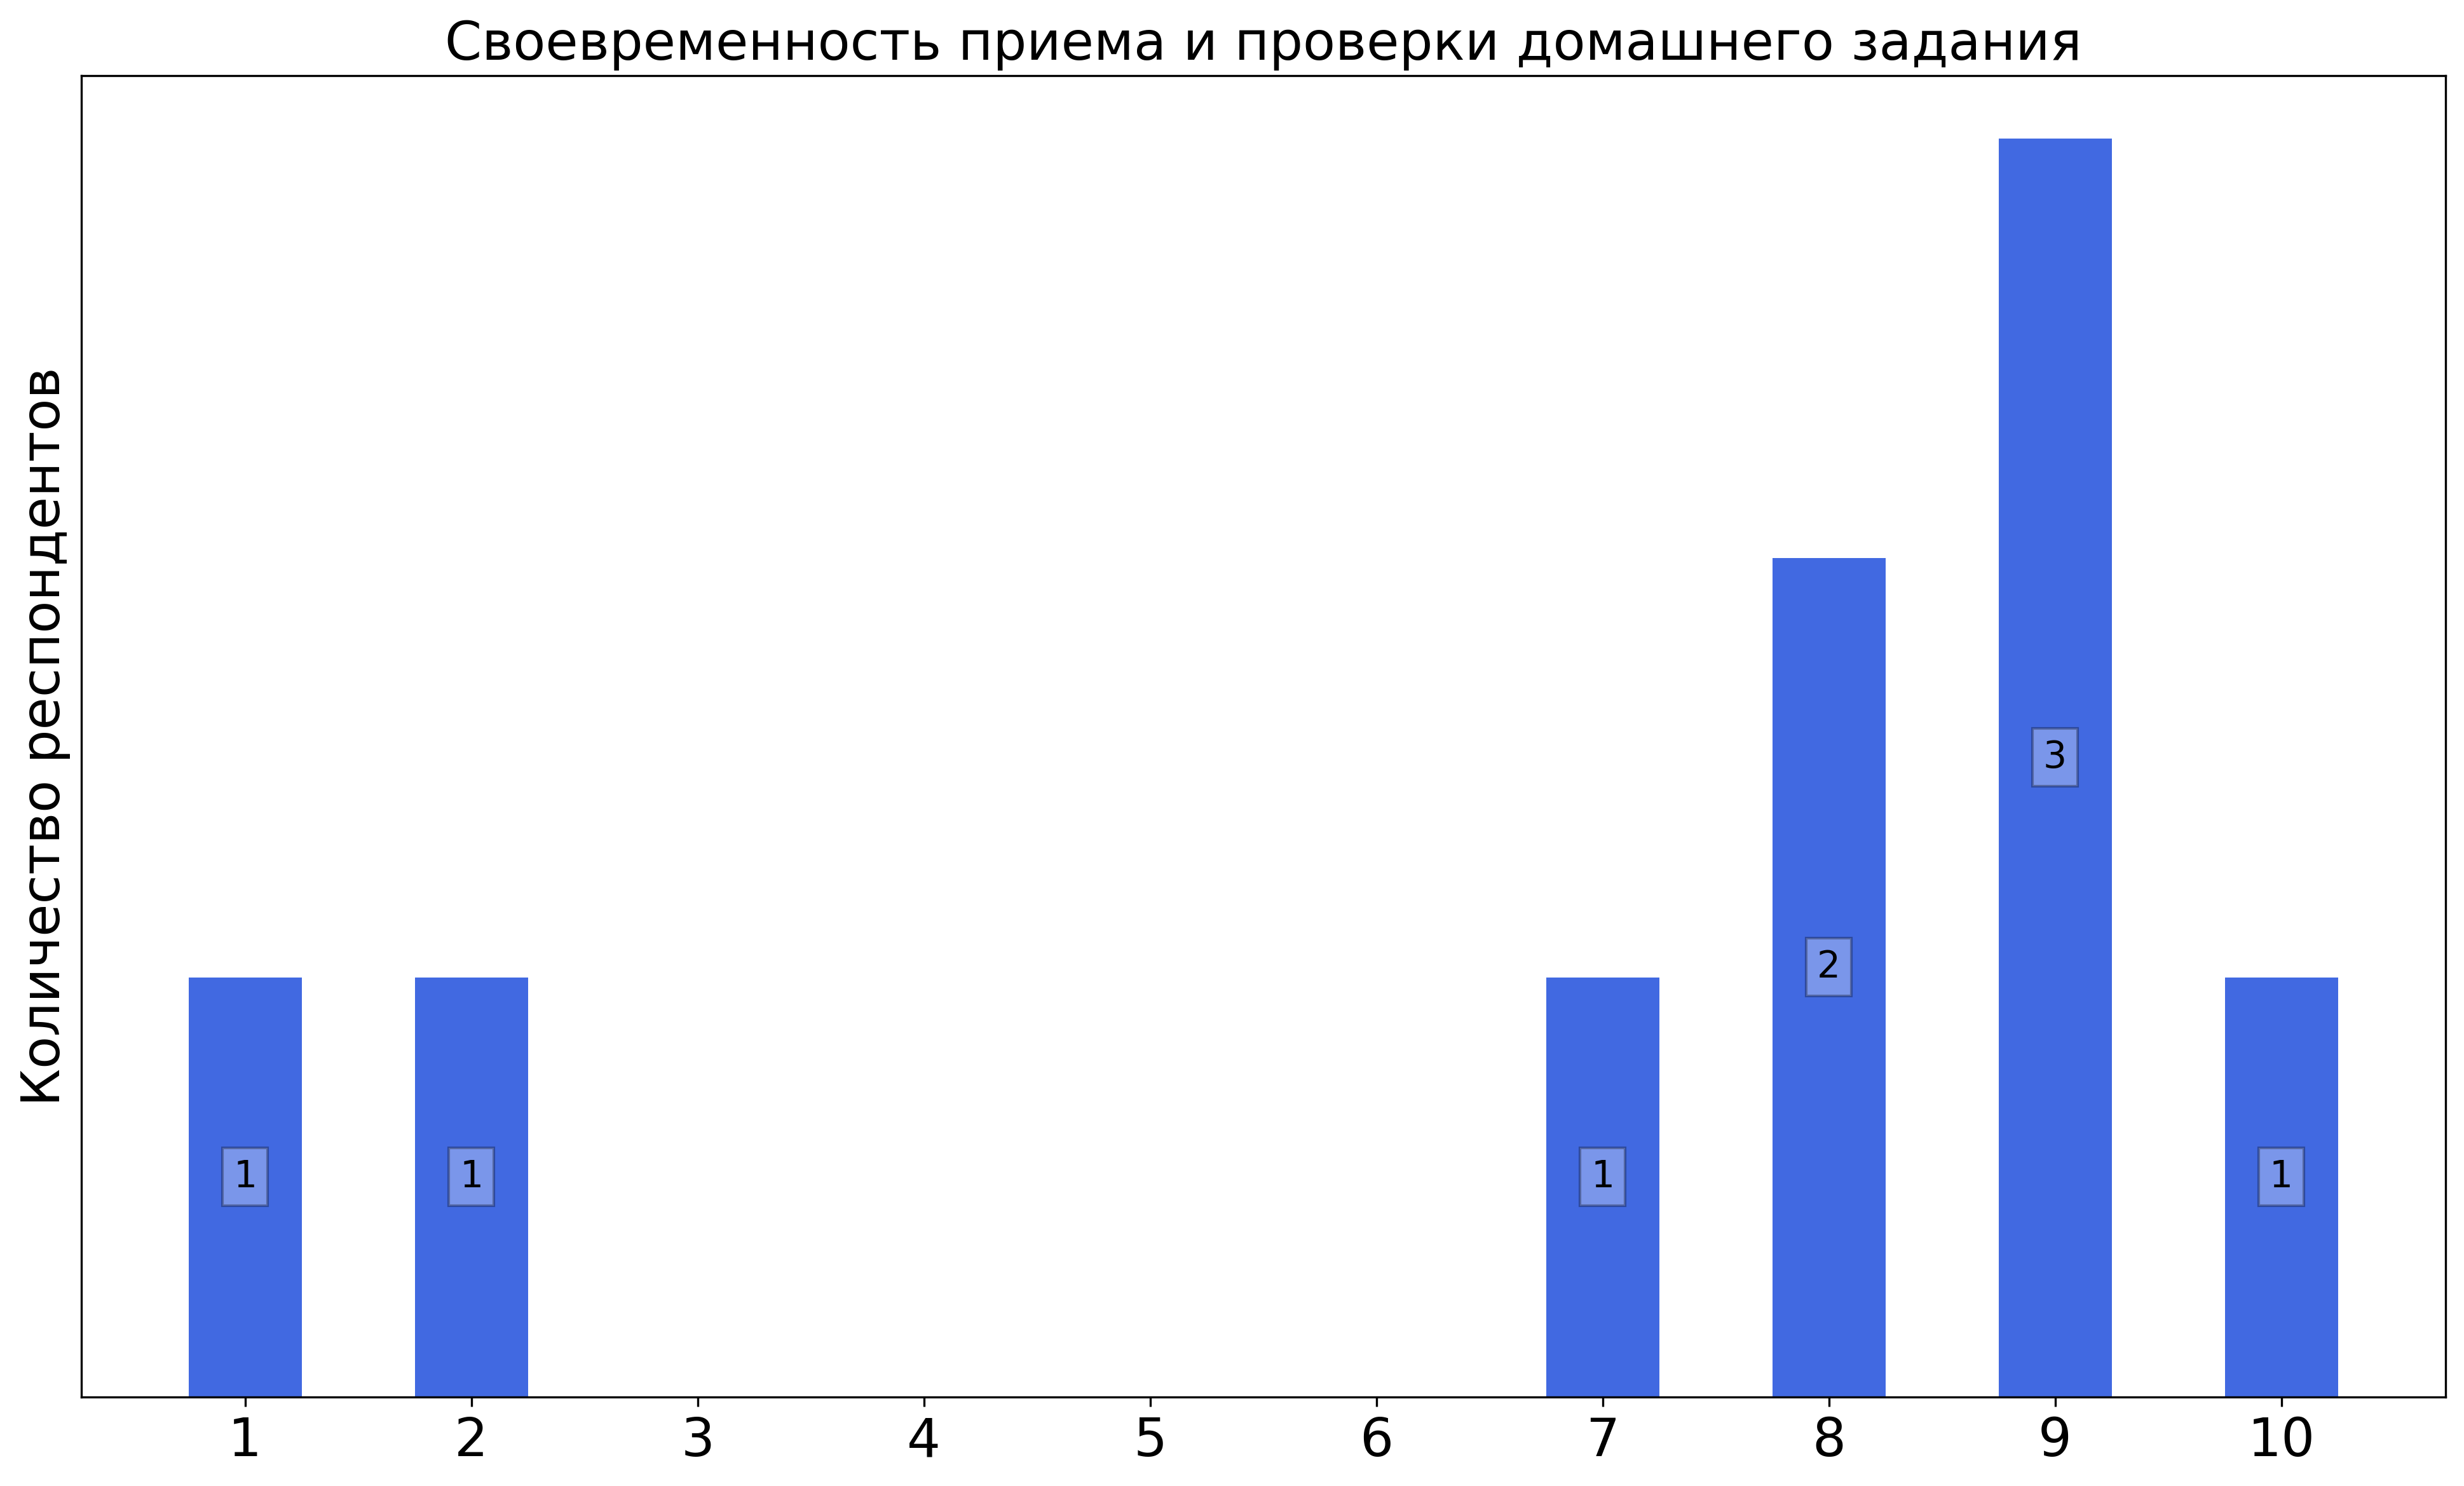
\includegraphics[width=\textwidth]{images/1 course/Информатика/seminarists-marks-Кулиев Р.С.-2.png}
            \end{subfigure}
            \begin{subfigure}[b]{0.45\textwidth}
                \centering
                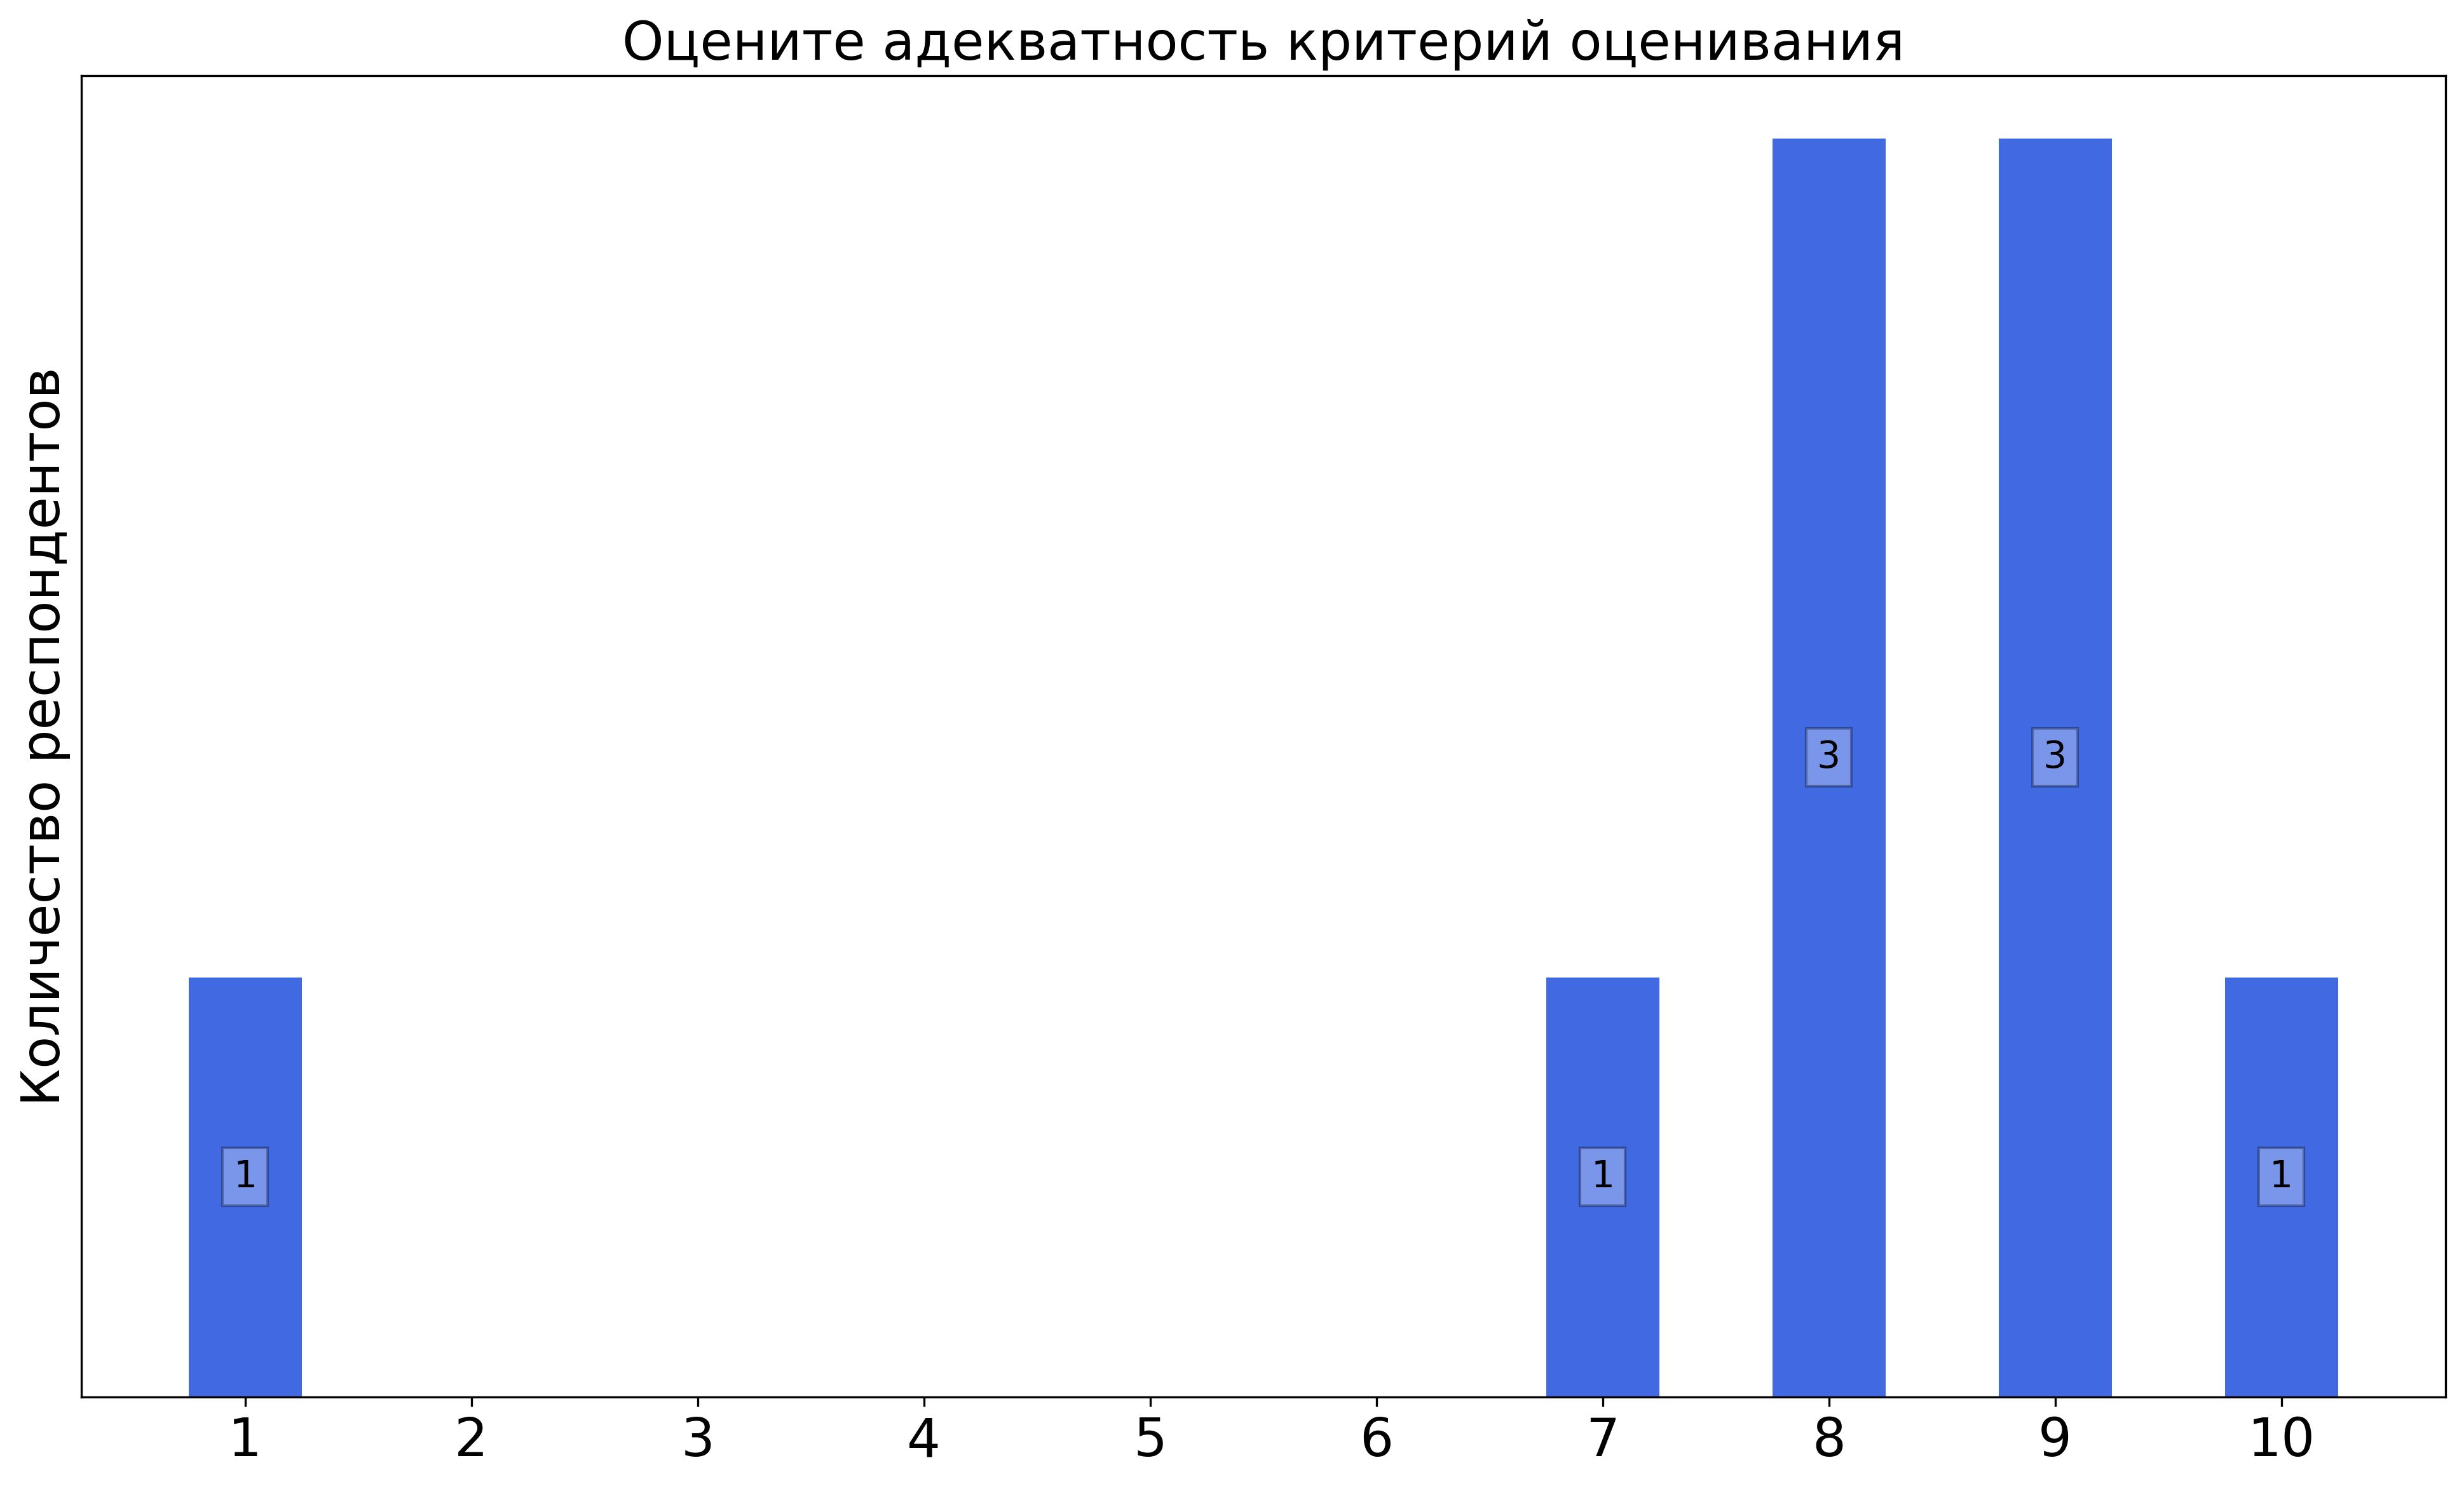
\includegraphics[width=\textwidth]{images/1 course/Информатика/seminarists-marks-Кулиев Р.С.-3.png}
            \end{subfigure}	
            \caption{Оценки респондентов о качестве преподавания семинаров}
        \end{figure}

        \textbf{Комментарии студентов о семинаристе\protect\footnote{сохранены оригинальные орфография и пунктуация}}
            \begin{commentbox} 
                Его постоянно нет на семинарах, он приходит на 5мин, говорит что нужно делать, потом уходит, приходит через час, спрашивает всё ли норм, посидит ещё полчаса и опять уйдёт.   
            \end{commentbox} 

    
    \subsubsection{Отзыв студентов о семинарах. Семинарист: Дивари И.Н.}
        \begin{figure}[H]
            \centering
            \begin{subfigure}[b]{0.45\textwidth}
                \centering
                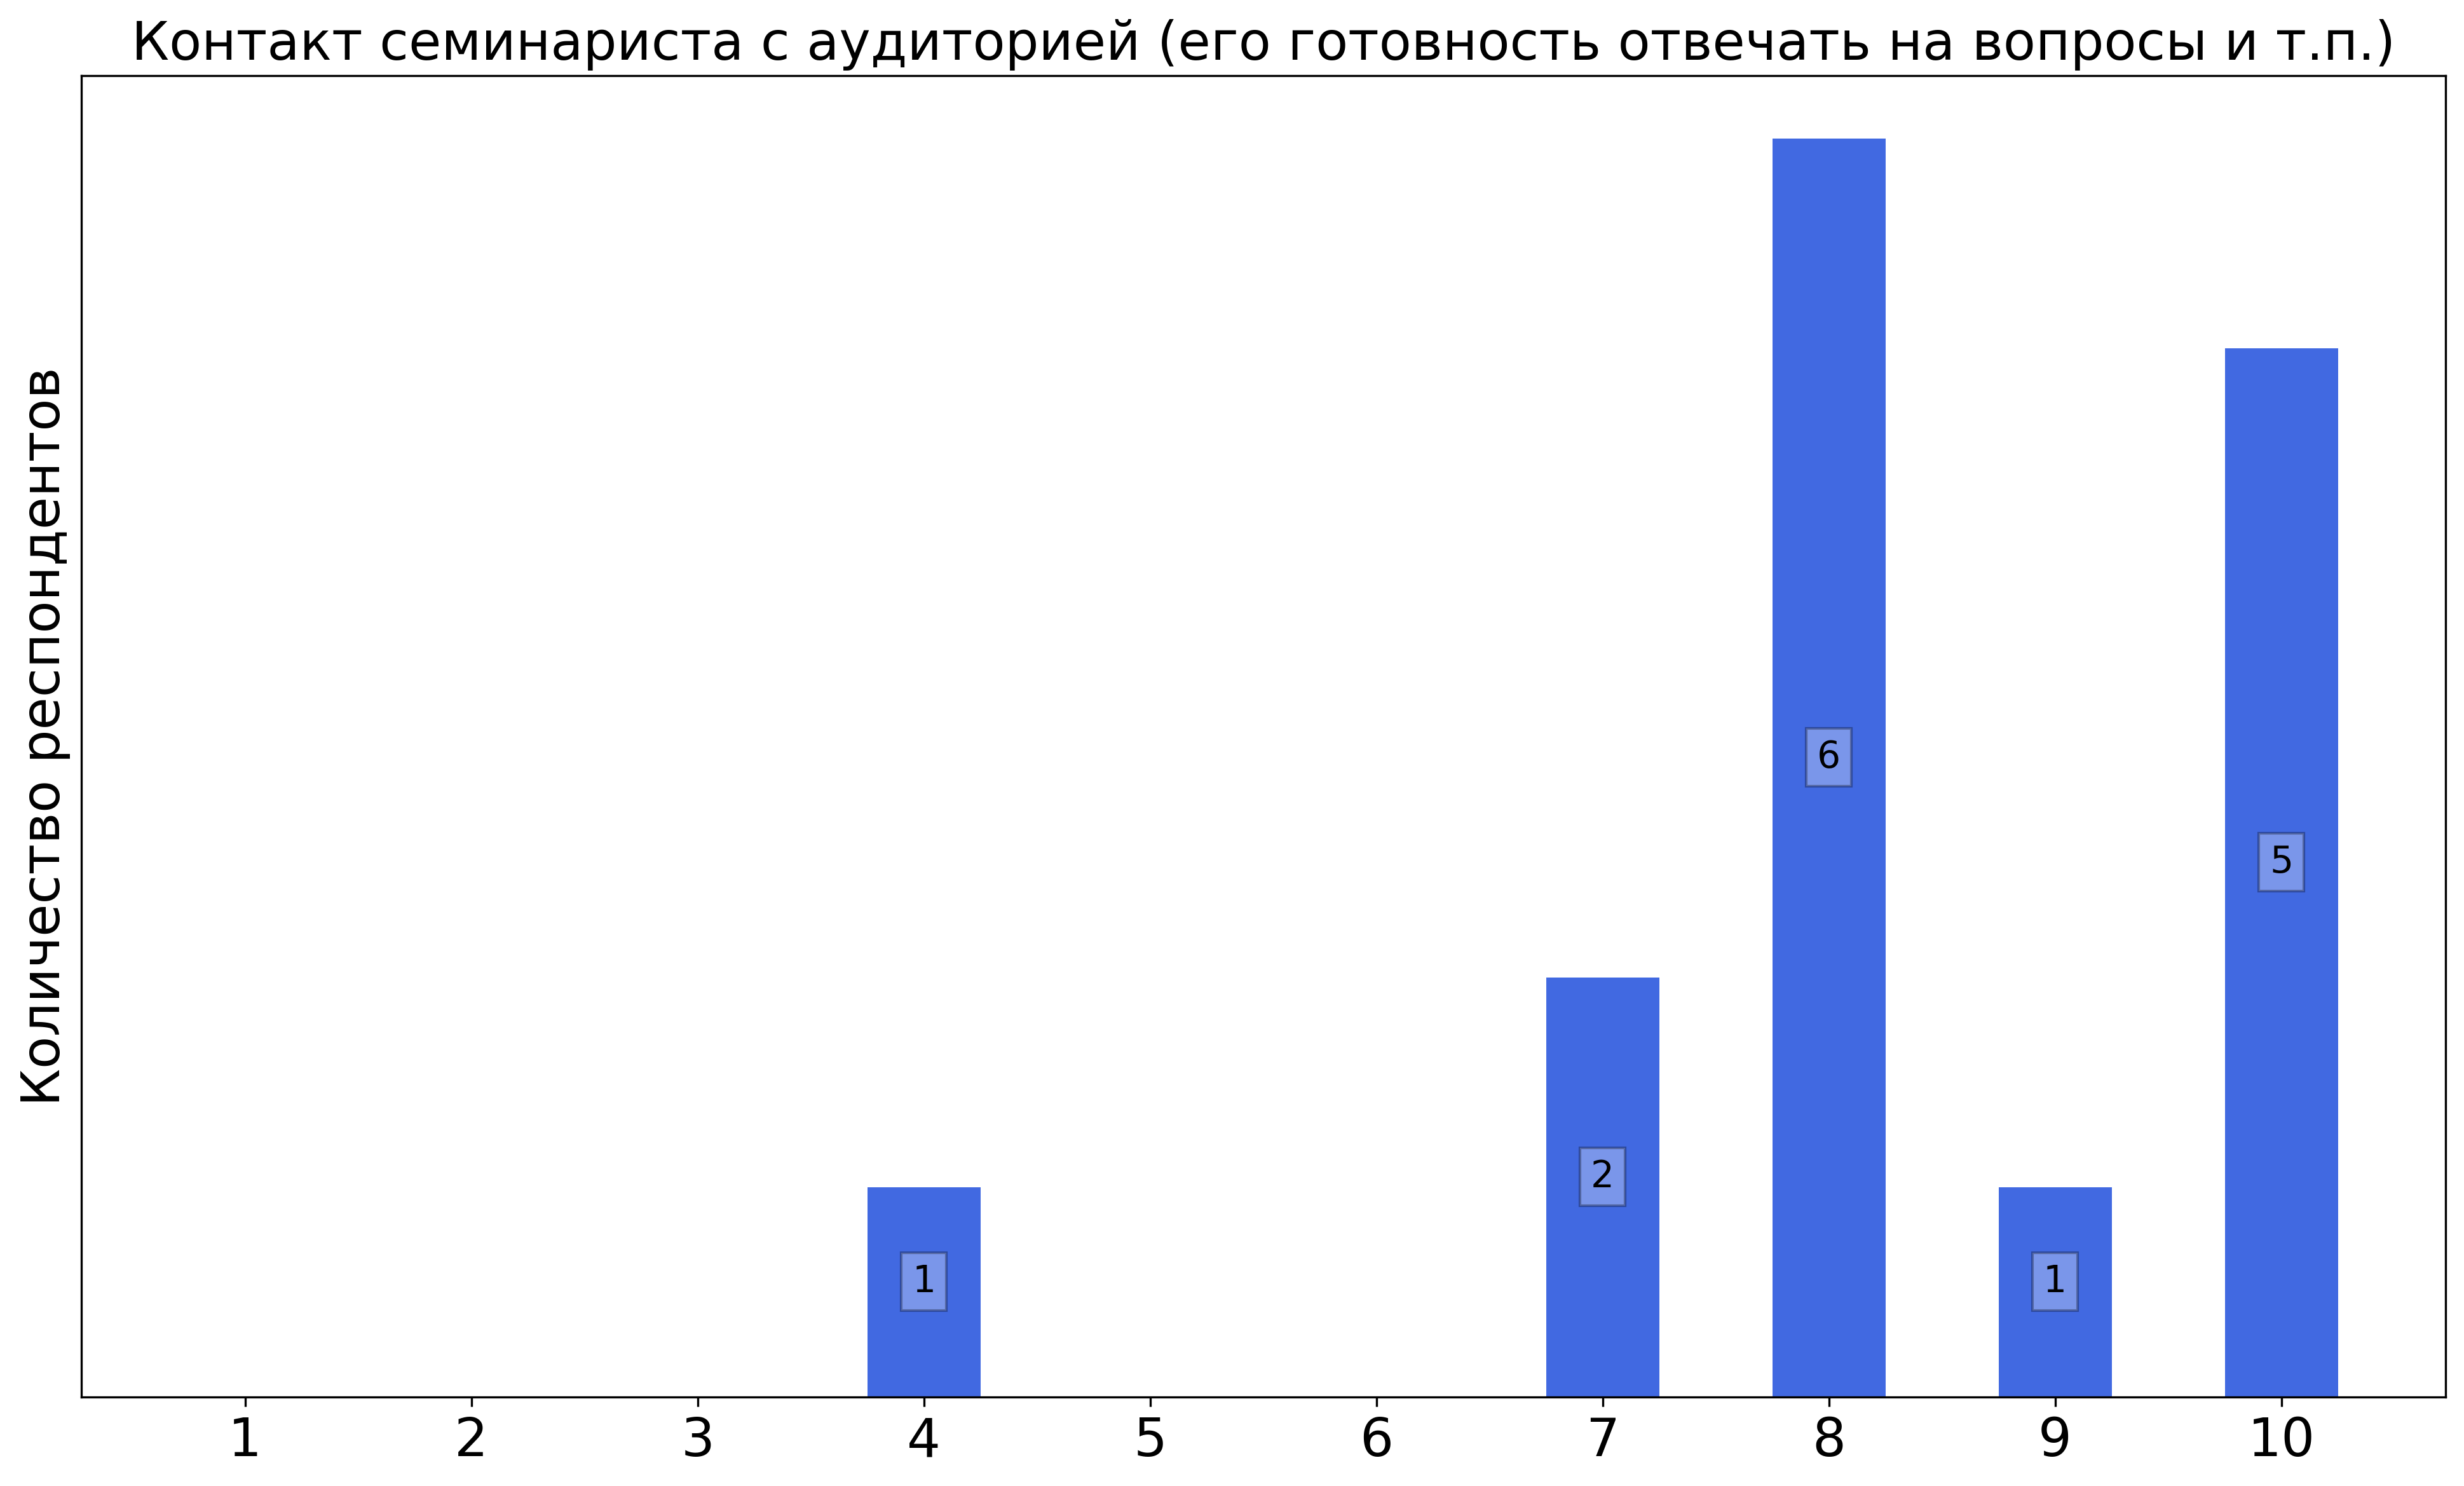
\includegraphics[width=\textwidth]{images/1 course/Информатика/seminarists-marks-Дивари И.Н.-0.png}
            \end{subfigure}
            \begin{subfigure}[b]{0.45\textwidth}
                \centering
                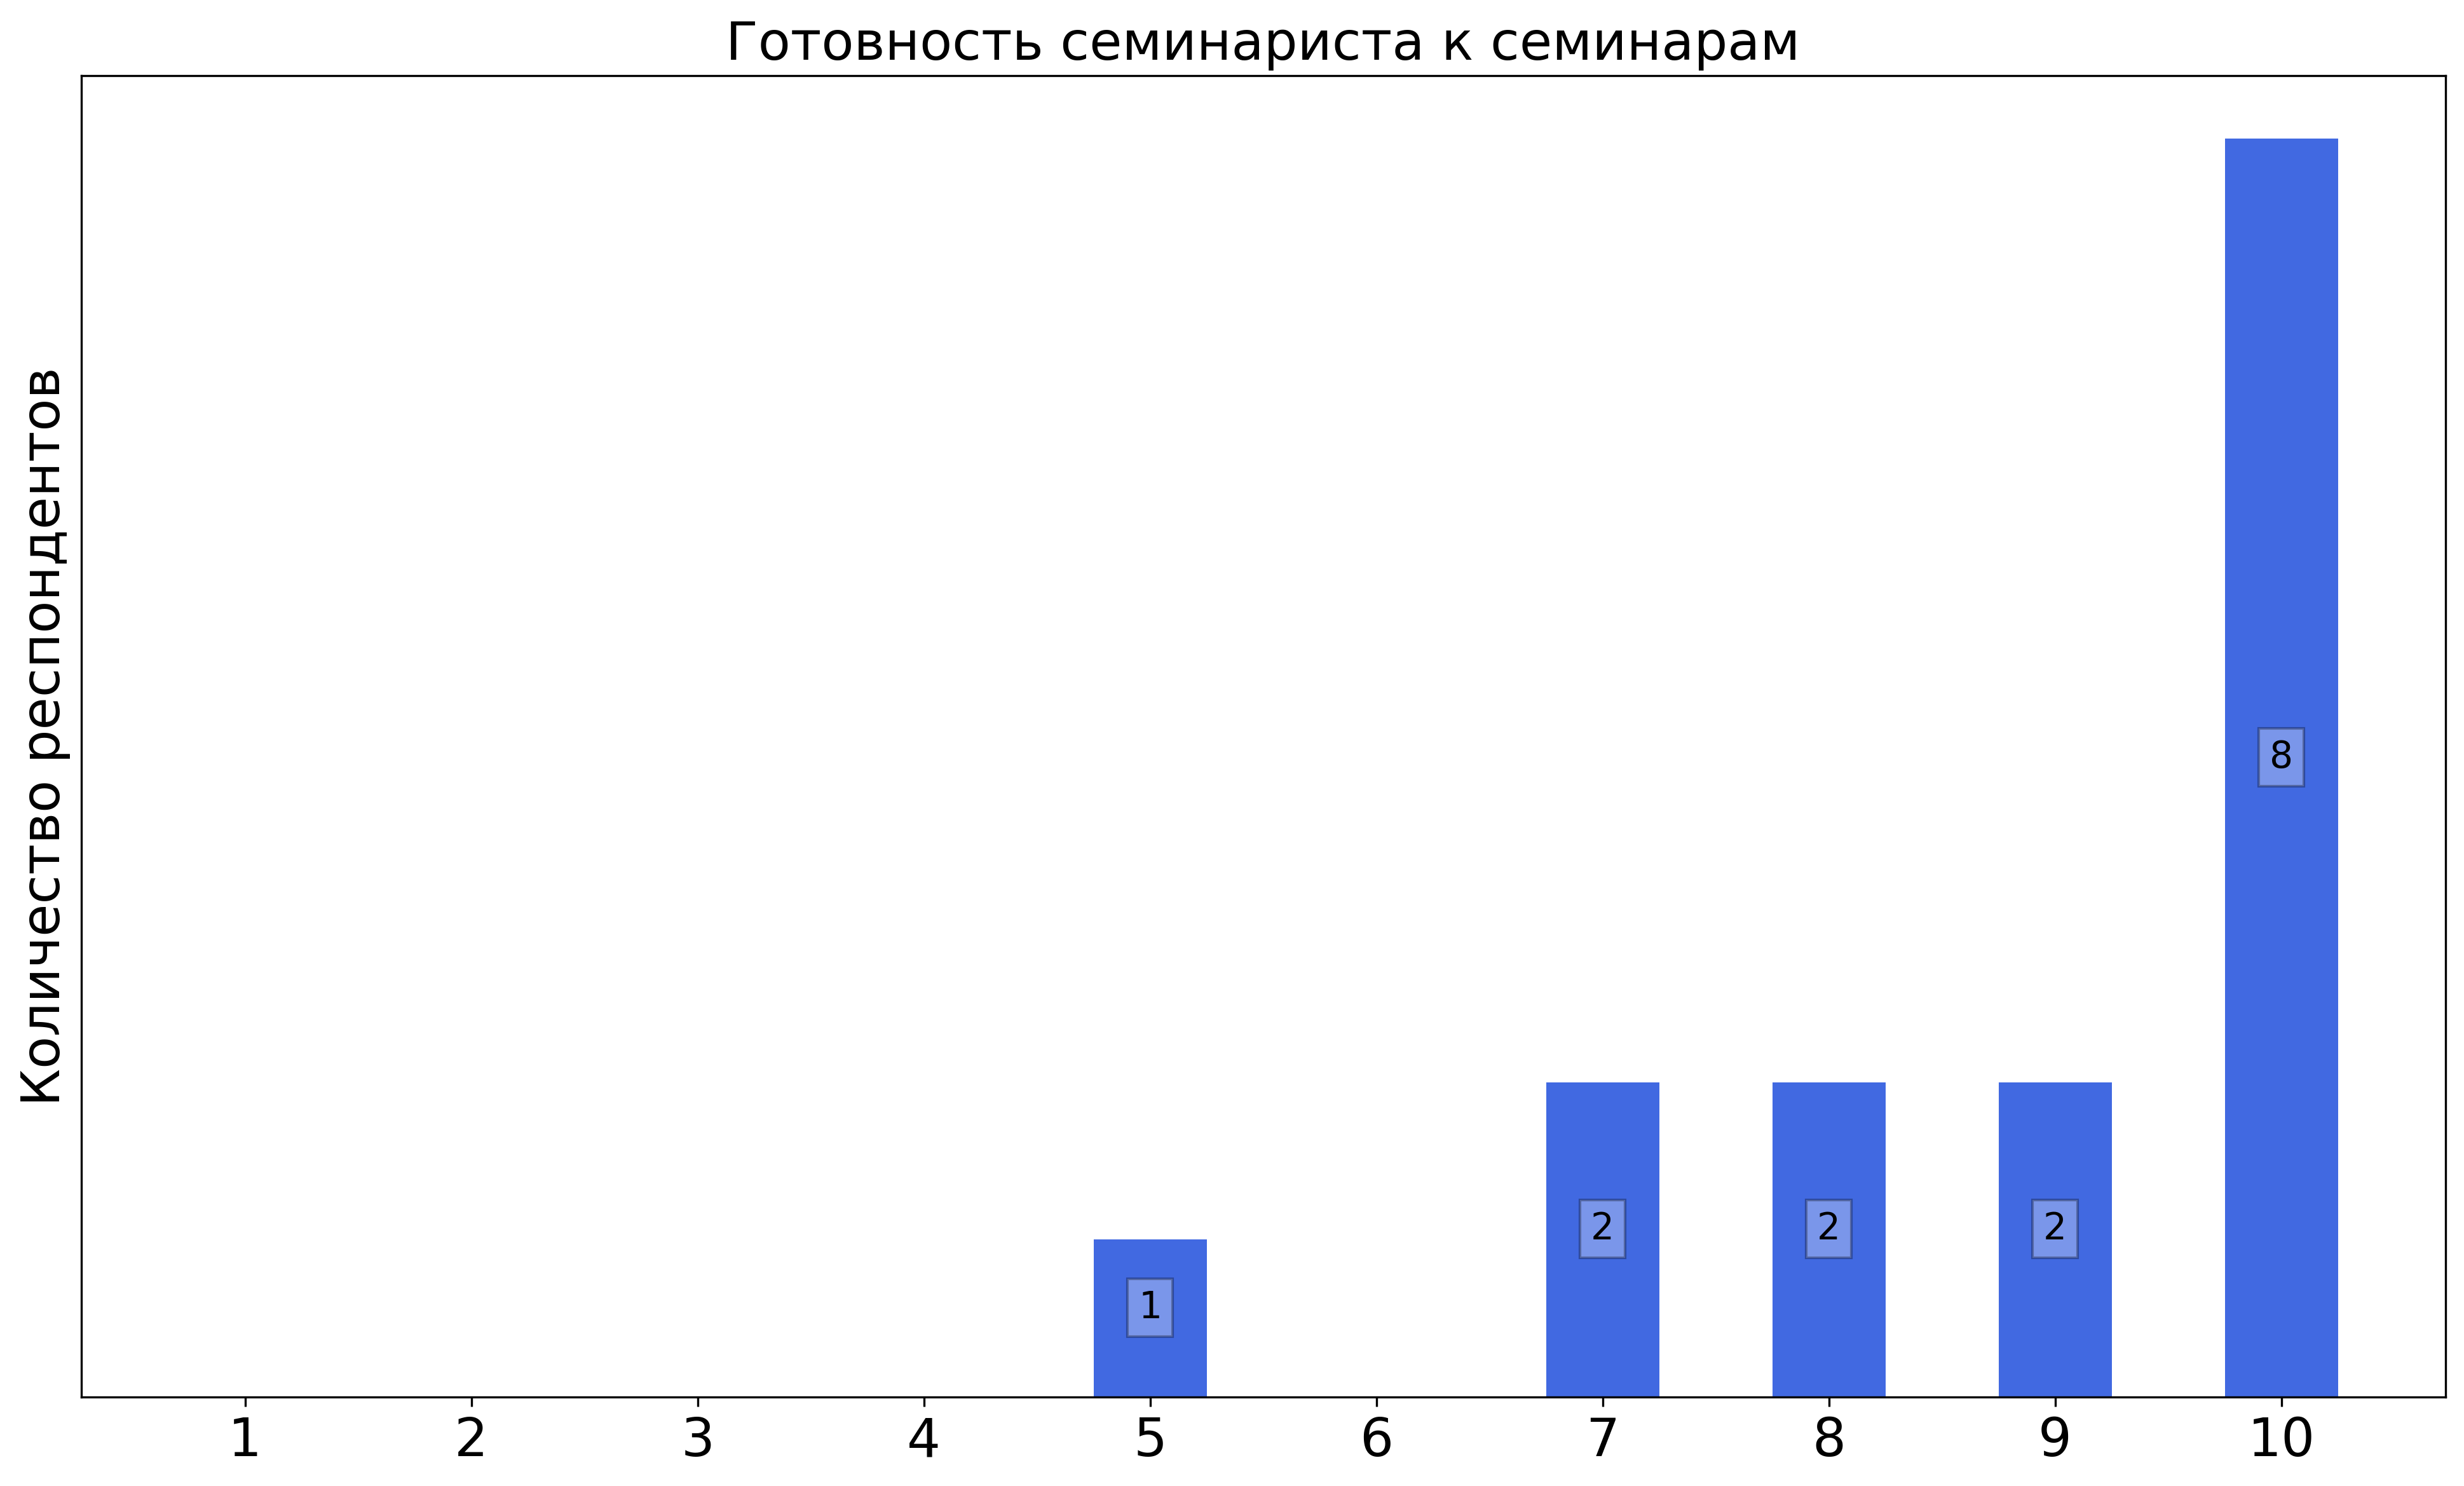
\includegraphics[width=\textwidth]{images/1 course/Информатика/seminarists-marks-Дивари И.Н.-1.png}
            \end{subfigure}
            \begin{subfigure}[b]{0.45\textwidth}
                \centering
                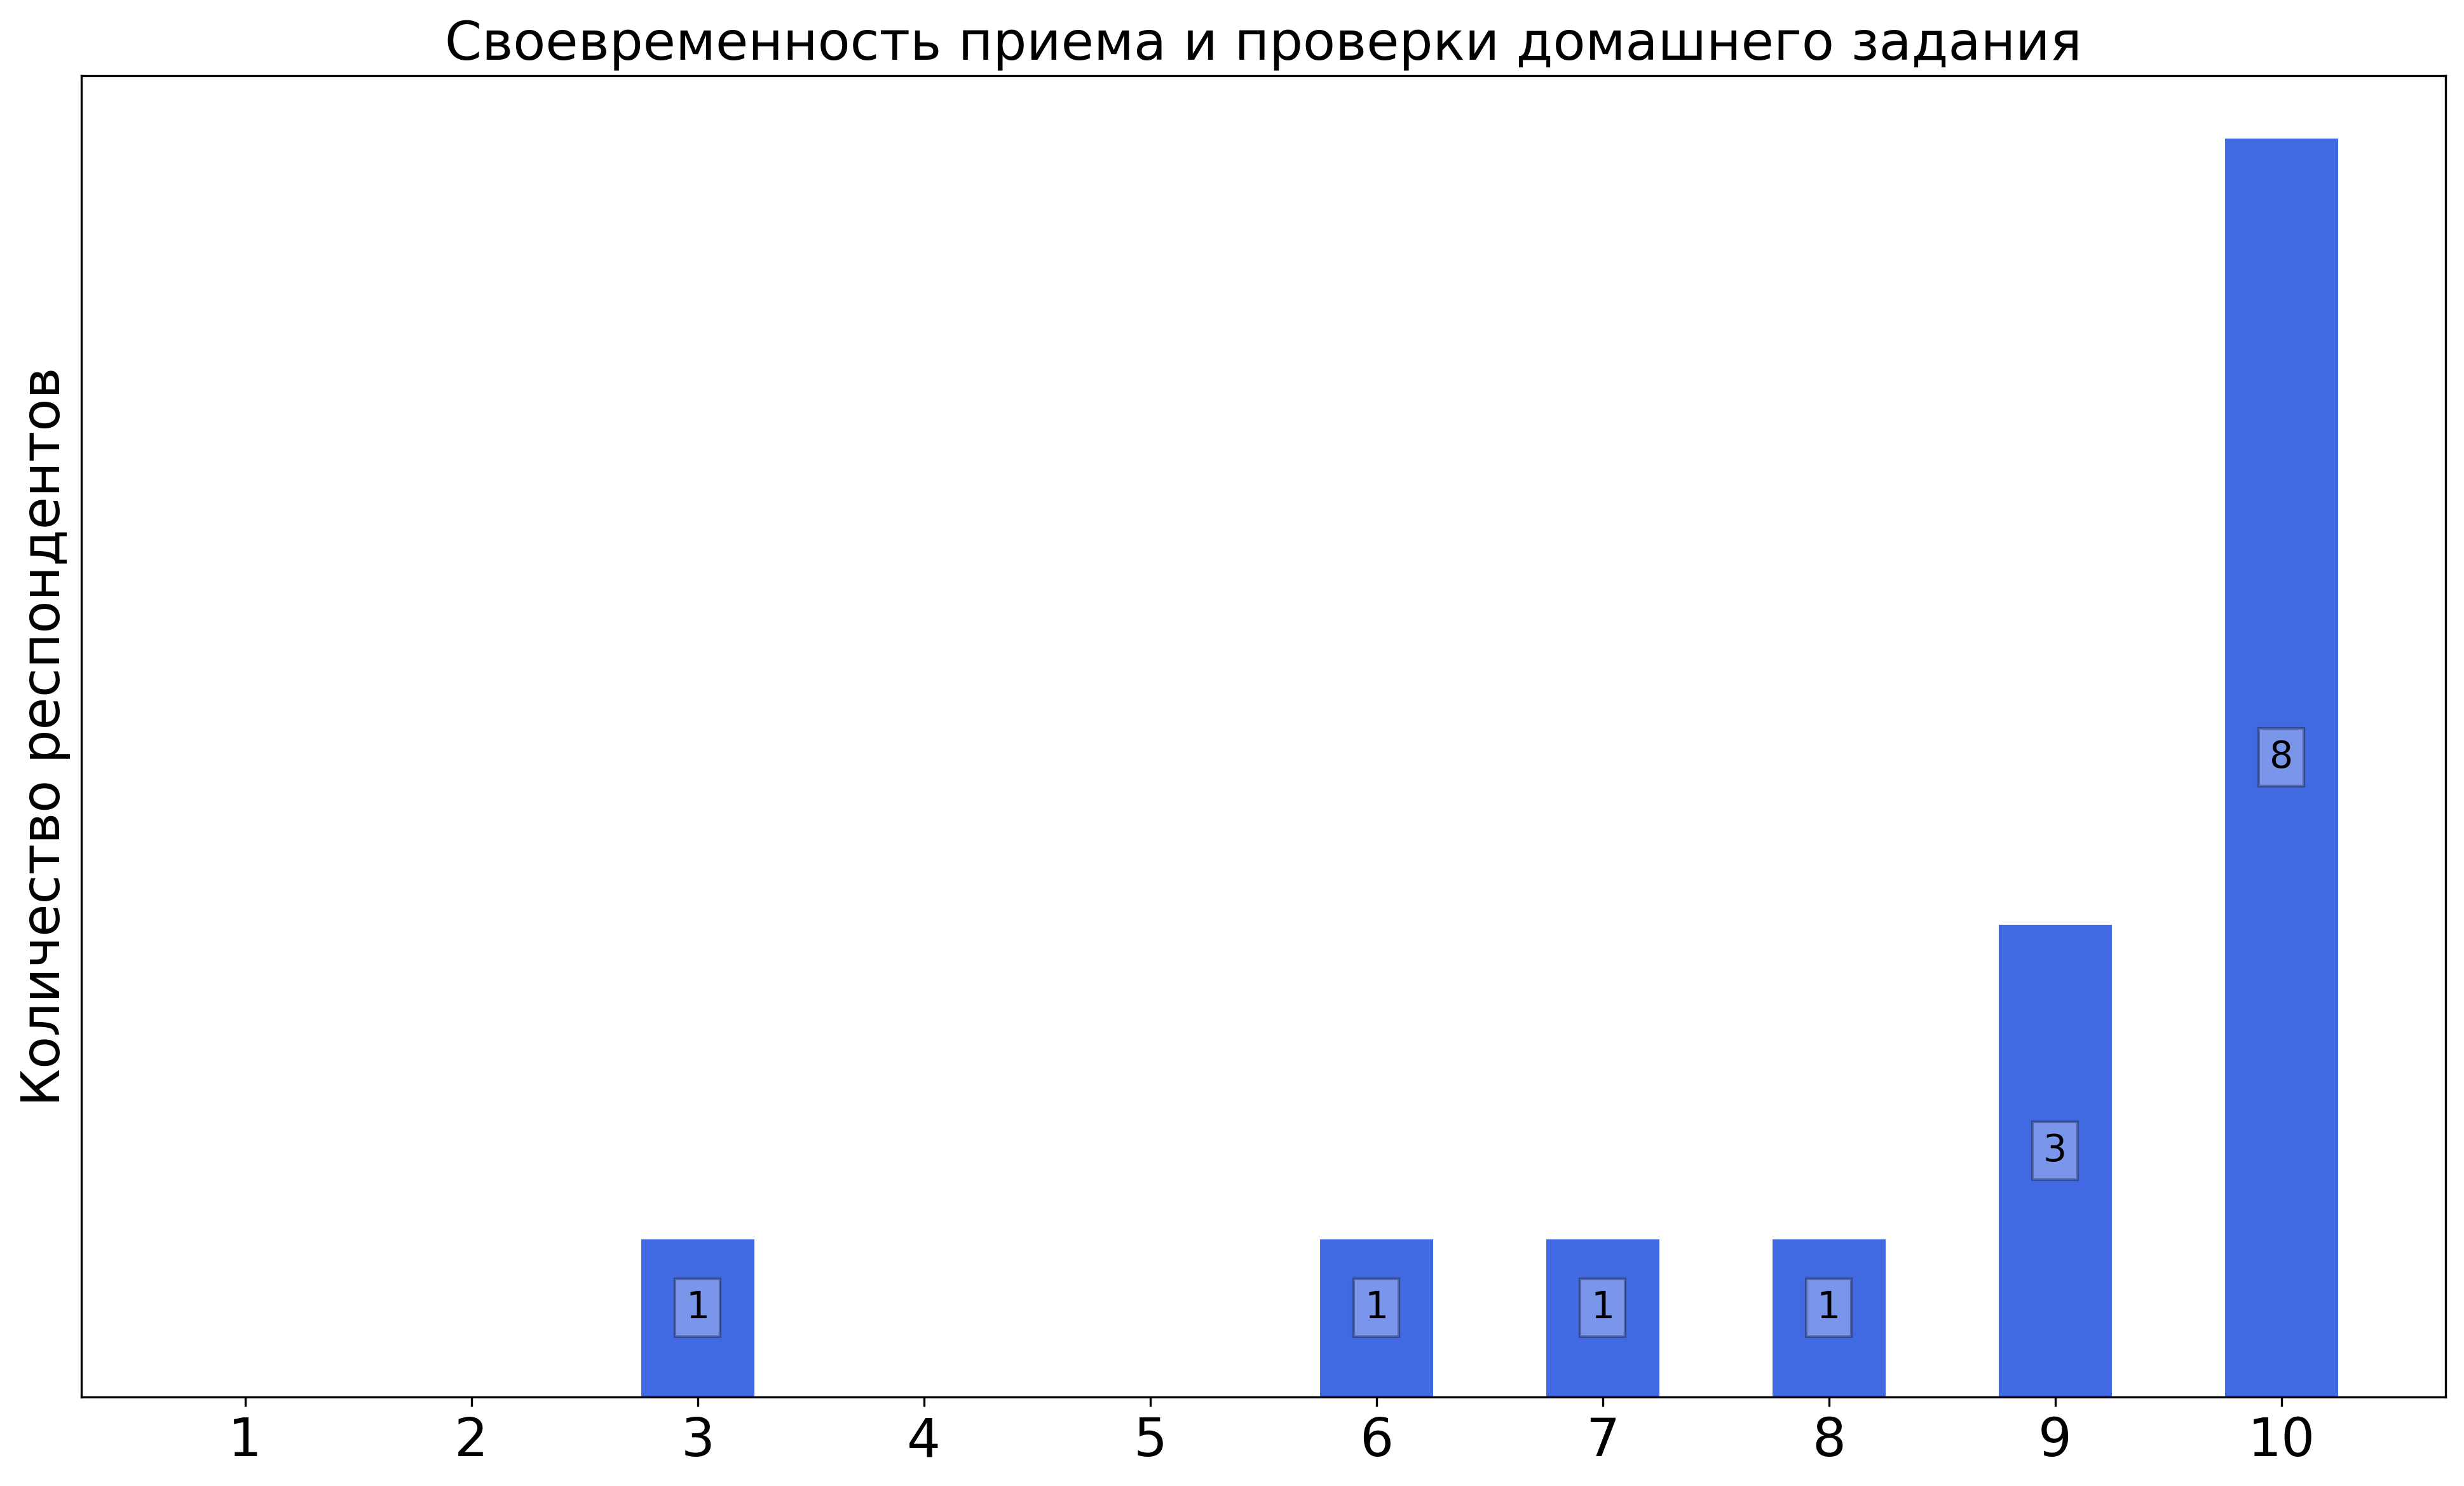
\includegraphics[width=\textwidth]{images/1 course/Информатика/seminarists-marks-Дивари И.Н.-2.png}
            \end{subfigure}
            \begin{subfigure}[b]{0.45\textwidth}
                \centering
                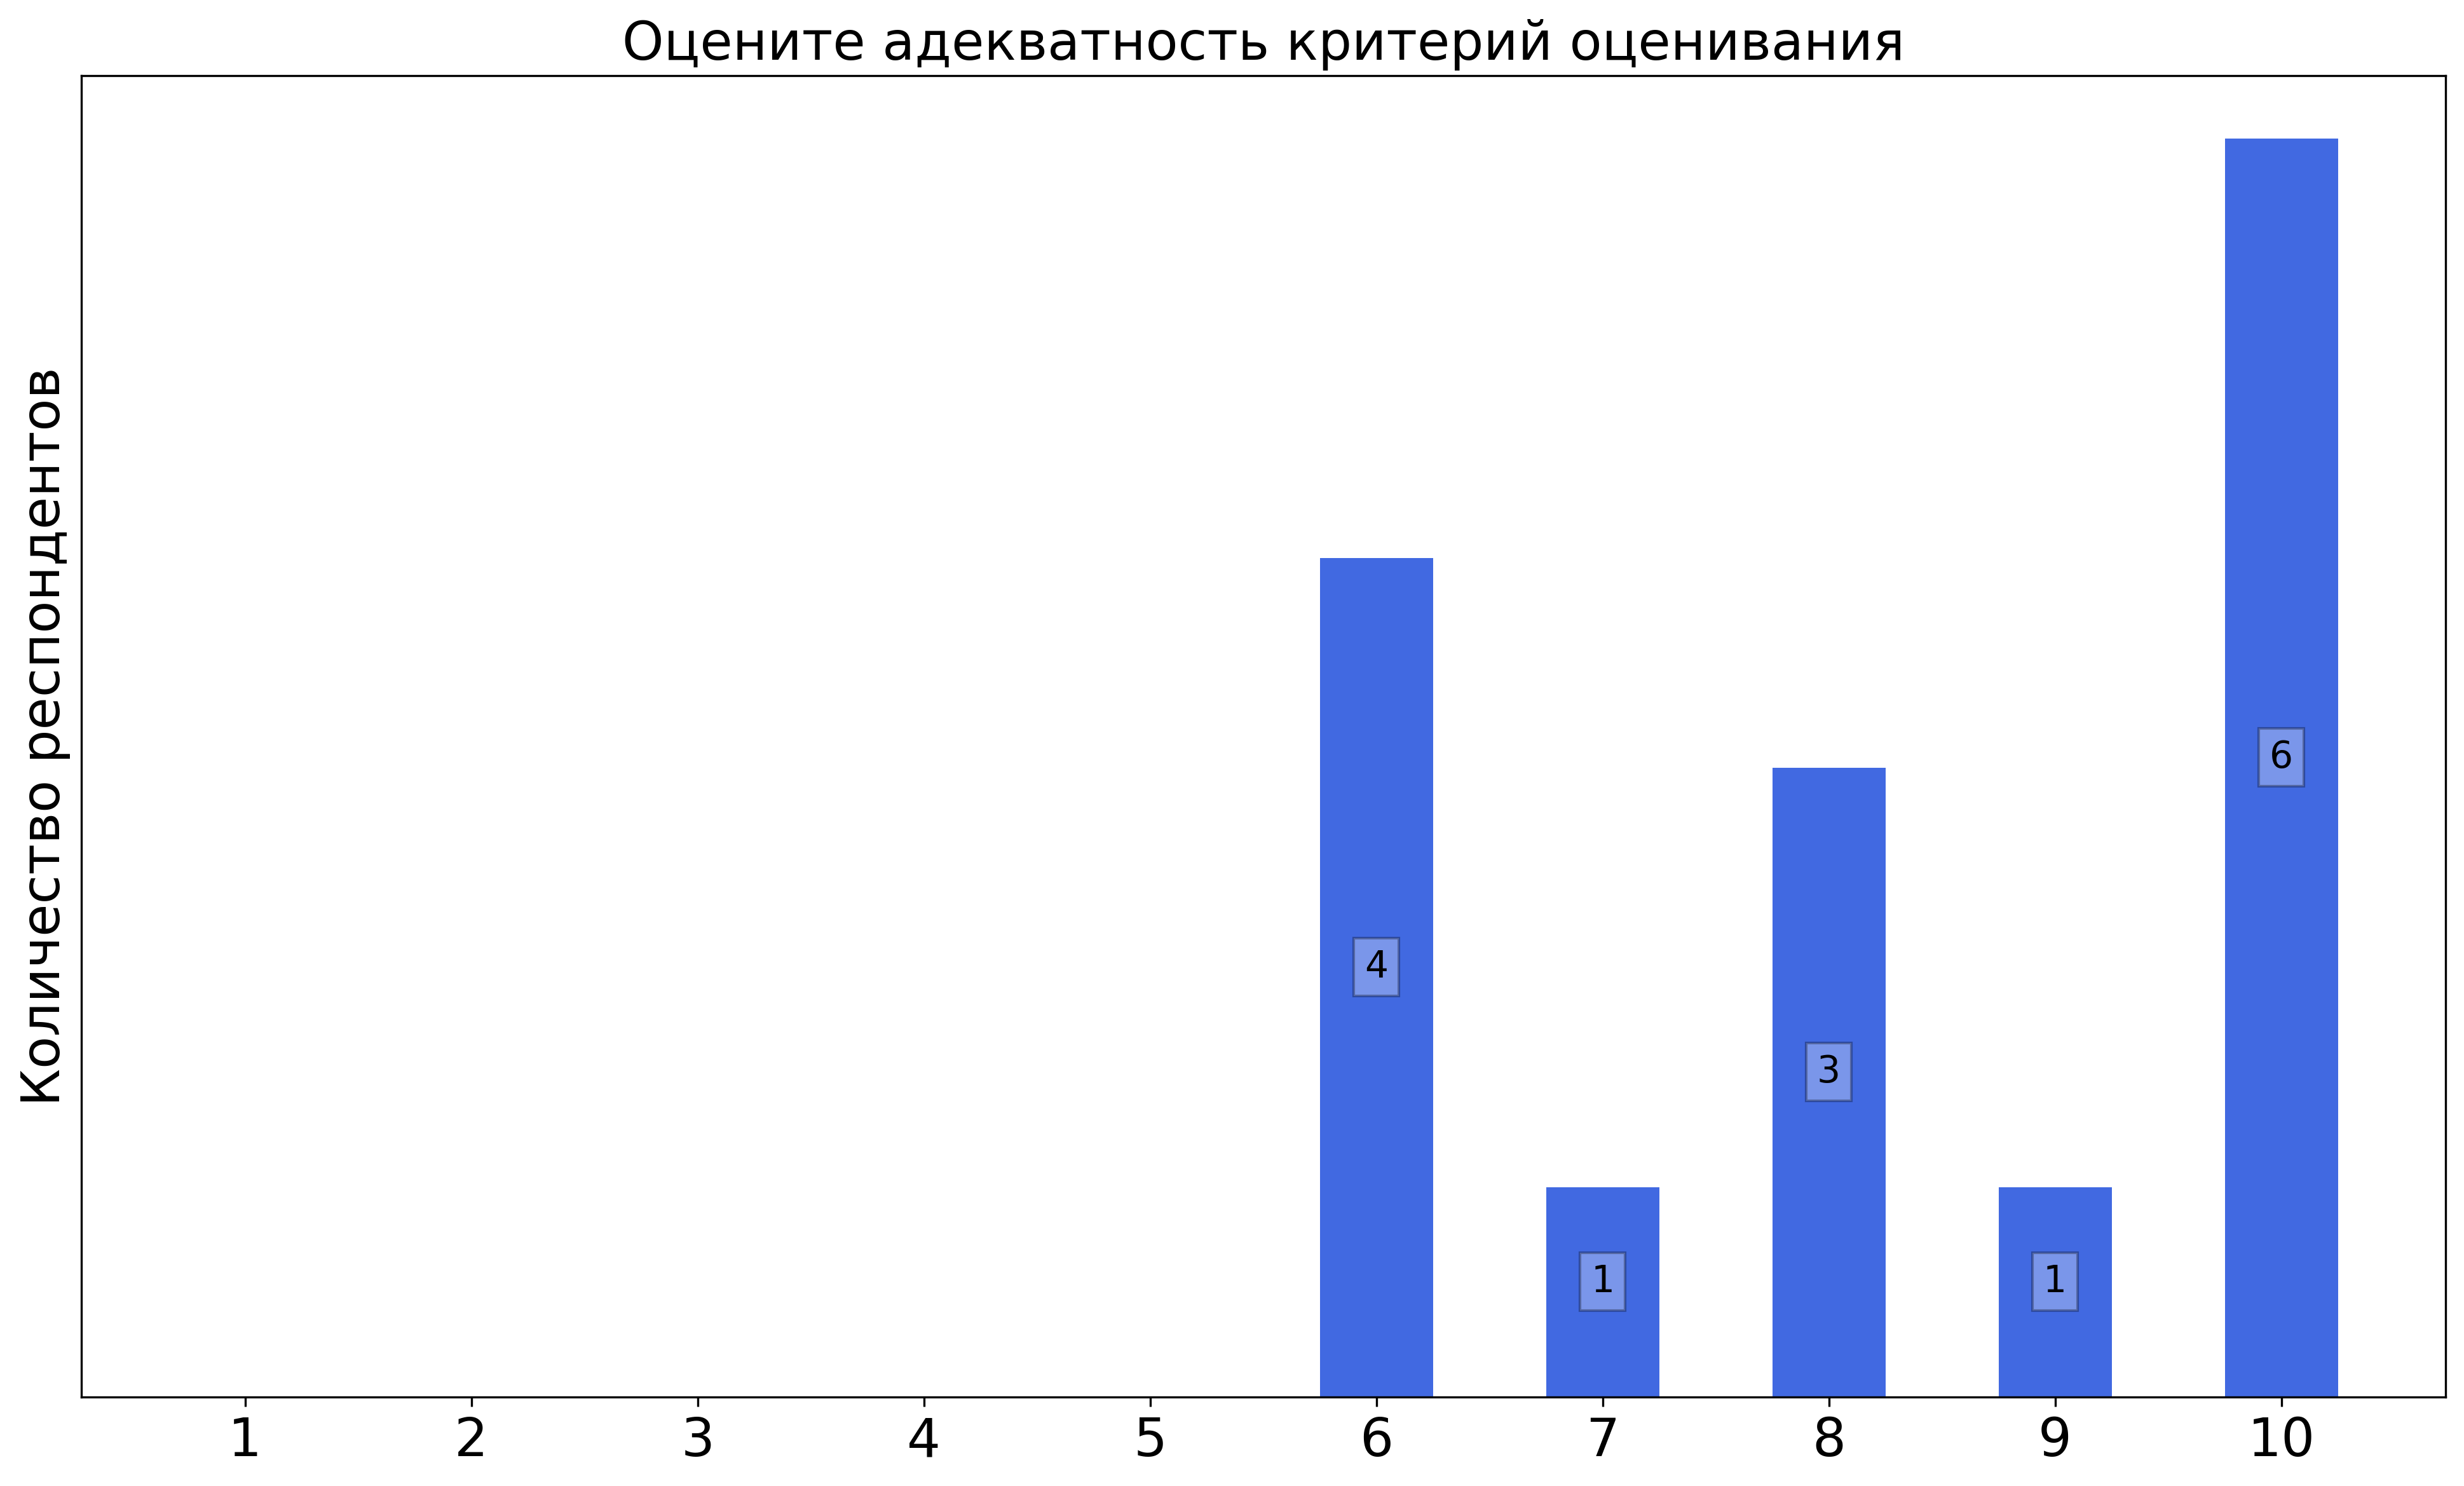
\includegraphics[width=\textwidth]{images/1 course/Информатика/seminarists-marks-Дивари И.Н.-3.png}
            \end{subfigure}	
            \caption{Оценки респондентов о качестве преподавания семинаров}
        \end{figure}

        \textbf{Комментарии студентов о семинаристе\protect\footnote{сохранены оригинальные орфография и пунктуация}}
            \begin{commentbox} 
                Даёт большое количество скучных и неинтересных задач, зачастую с очень странными формулировками, понятными одной лишь ей. Запрещает использовать то, что ещё не рассказала на лекциях. Я искренне не понимаю, зачем мне копировать массив побайтово, если существует memcpy. Весь семинар ты интенсивно пишешь код, в результате чего сильно устаешь, при этом почти не узнавая нового. Зачастую достаточно агрессивна по отношению к студентам. Из плюсов: охотно отвечает на вопросы, может научить чему-то, если студент не посещает доп. курсы. 
            \end{commentbox} 
        
            \begin{commentbox} 
                На хуавеи шли вперёд поэтому весь материал воспринимался достаточно легко  
            \end{commentbox} 
        
            \begin{commentbox} 
                Иногда не очень понятно формулирует задания. 
            \end{commentbox} 

    
    \subsubsection{Прочие комментарии и предложения по улучшению курса}
        \begin{commentbox}
            Лекции и хороший семинарист + допы отлично заходят, можно много разного узнать и закрепить
        \end{commentbox}

        \begin{commentbox}
            Было довольно странно, когда кафедра информатики не смогла нормально организовать семестровую контрольную.
        \end{commentbox}

        \begin{commentbox}
            Было бы просто ИДЕАЛЬНО, если бы Дед вёл свои лекции вместо обычных лекций по информатике, а семинары были бы всеобщим менторингом, что вполне осуществимо, так как семинары по информатике и так у всех в одно время.
        \end{commentbox}

        \begin{commentbox}
            Ничего не менять!
        \end{commentbox}

        \begin{commentbox}
            Добавьте алгосы уже емае. А то на вопрос, почему у нас их нет, ответ "Ну.. у вас есть курс под названием Информатика, которая вроде как их включает"
        \end{commentbox}

        \begin{commentbox}
            Доп. Курс Хуавей от Дединского - лучшее, что случалось с программированием на РТ
        \end{commentbox}